%\documentclass[acmsmall,screen]{acmart}
\documentclass[acmsmall,review,anonymous]{acmart}\settopmatter{printfolios=true,printccs=false,printacmref=false}
\usepackage{parskip}
\usepackage{caption, subcaption}
\usepackage{algorithm, algpseudocode}
\usepackage{tikz}
\usetikzlibrary{arrows,automata,positioning,backgrounds,calc,patterns}
\usetikzlibrary{arrows.meta}
\usepackage{mathpartir}
\usepackage{framed}
\usepackage{ulem}


\tikzset{transaction state/.style={draw=black!0}}
\tikzset{
	arrow/.pic={\path[tips,every arrow/.try,->,>=#1] (0,0) -- +(.1pt,0);},
	pics/arrow/.default={triangle 90},
	lab dis/.store in=\LabDis,
	lab dis=0.3,
	->-/.style args={at #1 with label #2}{decoration={
			markings,
			mark=at position #1 with {\arrow{>}; \node at (0,\LabDis) {#2};}},postaction={decorate}},
	-<-/.style args={at #1 with label #2}{decoration={
			markings,
			mark=at position #1 with {\arrow{<}; \node at (0,\LabDis)
				{#2};}},postaction={decorate}},
	-*-/.style={decoration={
			markings,
			mark=at position #1 with {\fill (0,0) circle (1.5pt);}},postaction={decorate}}
}

%% Journal information
%% Supplied to authors by publisher for camera-ready submission;
%% use defaults for review submission.
\acmJournal{PACMPL}
\acmVolume{1}
\acmNumber{CONF} % CONF = POPL or ICFP or OOPSLA
\acmArticle{1}
\acmYear{2018}
\acmMonth{1}
\acmDOI{} % \acmDOI{10.1145/nnnnnnn.nnnnnnn}
\startPage{1}

%% Copyright information
%% Supplied to authors (based on authors' rights management selection;
%% see authors.acm.org) by publisher for camera-ready submission;
%% use 'none' for review submission.
\setcopyright{none}
%\setcopyright{acmcopyright}
%\setcopyright{acmlicensed}
%\setcopyright{rightsretained}
%\copyrightyear{2018}           %% If different from \acmYear

%% Bibliography style
\bibliographystyle{ACM-Reference-Format}
%% Citation style
%% Note: author/year citations are required for papers published as an
%% issue of PACMPL.
\citestyle{acmauthoryear}   %% For author/year citations


%%%%%%%%%%%%%%%%%%%%%%%%%%%%%%%%%%%%%%%%%%%%%%%%%%%%%%%%%%%%%%%%%%%%%%
%% Note: Authors migrating a paper from PACMPL format to traditional
%% SIGPLAN proceedings format must update the '\documentclass' and
%% topmatter commands above; see 'acmart-sigplanproc-template.tex'.
%%%%%%%%%%%%%%%%%%%%%%%%%%%%%%%%%%%%%%%%%%%%%%%%%%%%%%%%%%%%%%%%%%%%%%





\definecolor{pinegreen}{rgb}{0.0, 0.47, 0.44}
\newcommand{\callout}[2][pinegreen]{\normalem{\emph{\textcolor{#1}{#2}}}\ULforem
}

\newenvironment{cframed}[1][black] {\def\FrameCommand{\fboxsep=\FrameSep\fcolorbox{#1}{white}}%
	\MakeFramed {\advance\hsize-\width \FrameRestore}}
{\endMakeFramed}

\newcommand{\rchange}[1]{#1}

\newcommand{\dipnote}[1]{{\color{red}{#1}}}
\newcommand{\constantin}[1]{{\color{red}{Constantin: #1}}}
\newcommand{\akash}[1]{{\color{red}{#1}}}

\newcommand{\figref}[1]{Figure~\ref{fig:#1}}
\newcommand{\sectref}[1]{\S\ref{sec:#1}}

\newcommand{\eg}{e.g., }
\newcommand{\ie}{i.e., }

\newcommand{\key}{x}
\newcommand{\Keys}{\mathsf{Vars}}
\newcommand{\Events}{\mathcal{E}}

\definecolor{coColor}{HTML}{b37200}
\definecolor{soColor}{HTML}{800080}
\definecolor{poColor}{HTML}{C41E3A}
\definecolor{wrColor}{HTML}{008000}
\definecolor{orColor}{HTML}{0026ff}

\newcommand{\PO}{\textcolor{poColor}{\textsf{po}}}
\newcommand{\SO}{\textcolor{soColor}{\textsf{so}}}
\newcommand{\WR}{\textcolor{wrColor}{\textsf{WR}}}
\newcommand{\WW}{\textcolor{red}{\textsf{WW}}}
\newcommand{\RW}{\textcolor{red}{\textsf{RW}}}
\newcommand{\VIS}{\textcolor{red}{\textsf{vis}}}
\newcommand{\CO}{\textcolor{coColor}{\textsf{co} }}

\newcommand{\axpre}{\mathsf{Prefix}}
\newcommand{\axconf}{\mathsf{Conflict}}
\newcommand{\axsi}{\textsc{Si}}
\newcommand{\axser}{\mathsf{Serializability}}

\newcommand{\ext}{\textsc{Ext}}
\newcommand{\session}{\textsc{Session}}
\newcommand{\transvis}{\textsc{TransVis}}
\newcommand{\prefix}{\textsc{Prefix}}
\newcommand{\noconflict}{\textsc{NoConflict}}
\newcommand{\totalvis}{\textsc{TotalVis}}

\newcommand{\set}[1]{{\{{#1}\}}}
\newcommand{\mset}[1]{{\{\!\{ #1 \}\!\}}}
\newcommand{\tup}[1]{{\left\langle{#1}\right\rangle}}
\renewcommand{\implies}{\Rightarrow}
\newcommand{\pto}{\rightharpoonup}
\newcommand{\To}{\Rightarrow}
\newcommand{\Path}[3]{{#1}\xrightarrow{#2}{#3}}


\newcommand{\Obj}{\mathsf{Obj}}
\newcommand{\Var}{\mathsf{Vars}}
\newcommand{\Vars}{\mathsf{Vars}}
\newcommand{\LVars}{\mathsf{LVars}}
\newcommand{\Val}{\mathsf{Vals}}
\newcommand{\Vals}{\mathsf{Vals}}
\newcommand{\Columns}{\mathbb{C}}
\newcommand{\Rows}{\mathbb{R}}
\newcommand{\Tables}{\mathbb{T}}
\newcommand{\OId}{\mathsf{OpId}}
\newcommand{\Op}{\mathsf{Op}}
\newcommand{\xvar}{{a}}
\newcommand{\prog}{{\mathsf{P}}}
\newcommand{\histOf}[2][]{{\mathsf{hist}_{#1}({#2})}}

\newcommand{\ebegin}{\mathsf{begin}}
\newcommand{\eend}{\mathsf{end}}
\newcommand{\erd}[1]{\mathsf{read}({#1})}
\newcommand{\ewrt}[1]{\mathsf{write}({#1})}

\newcommand{\yvar}{{y}}
\newcommand{\val}{{v}}
\newcommand{\id}{{i}}
\newcommand{\rd}[2][]{\textsf{read}_{#1}({#2})}
%\newcommand{\rd}[3][]{\textsf{read}_{#1}({#2},{#3})}
\newcommand{\rdo}{\textsf{read}}
\newcommand{\wrt}[3][]{\textsf{write}_{#1}({#2},{#3})}
\newcommand{\op}{{o}}
\newcommand{\Tr}{{\mathcal{T}}}
\newcommand{\tr}{t}
\newcommand{\Hist}{{\mathcal{H}}}
\newcommand{\hist}{{h}}
\newcommand{\po}{\textcolor{poColor}{\mathsf{po}}}
\newcommand{\so}{\textcolor{soColor}{\mathsf{so}}}
\newcommand{\co}{\textcolor{coColor}{\mathsf{co}}}
\newcommand{\ora}{\textcolor{orColor}{\mathsf{or}}}
\newcommand{\wro}{\textcolor{wrColor}{\mathsf{wr}}}
\newcommand{\rwo}{\mathsf{RW}}
\newcommand{\wrosi}{\mathsf{WR}}
\newcommand{\readOp}[1]{\mathsf{reads}({#1})}
\newcommand{\tlogs}[1]{\mathsf{TLogs}({#1})}
\newcommand{\transC}[1]{\mathsf{compTrans}({#1})}
\newcommand{\vars}[1]{\mathsf{vars}({#1})}
\newcommand{\writeOp}[1]{\mathsf{writes}({#1})}
\newcommand{\writeVar}[2]{{#1}\ \mathsf{writes}\ {#2}}
\newcommand{\readVar}[2]{{#1}\ \mathsf{reads}\ {#2}}
\renewcommand{\hist}{{h}}
\newcommand{\lin}{\textcolor{red}{\mathsf{lin}}}
\newcommand{\vis}{\textcolor{red}{\mathsf{vis}}}
\newcommand{\aread}{\mathsf{r}}
\newcommand{\none}{\mathsf{None}}
\newcommand{\btrue}{\mathsf{true}}
\newcommand{\bfalse}{\mathsf{false}}

\newcommand{\trans}[2]{\mathsf{trans}({#1},{#2})}

%---- Models
\newcommand{\CC}{\textup{\texttt{CC}}}
\newcommand{\SER}{\textup{\texttt{SER}}}
\newcommand{\PRE}{\textup{\texttt{PRE}}}
\newcommand{\SI}{\textup{\texttt{SI}}}
\newcommand{\RA}{\textup{\texttt{RA}}}
\newcommand{\RC}{\textup{\texttt{RC}}}

%---- Basic definitions

\newcommand{\init}{\textup{\textbf{\texttt{init}}}}
\newcommand{\type}[1]{\textup{\texttt{type}}(#1)}

%---- Theoretical algorithm

\newcommand{\locals}{\mathsf{locals}}
\newcommand{\genericNext}{\textsc{Next}}
\newcommand{\genericEvaluate}{\textsc{Final}}
\newcommand{\genericCompute}{\textsc{ComputeReordering}}
\newcommand{\genericProtocol}{\textsc{OptimalityCondition}}
\newcommand{\genericSwap}{\textsc{Swap}}
\newcommand{\genericValidWrites}{\textsc{ValidWrites}}
\newcommand{\nextEvent}{\textup{\textsc{next}}}
\newcommand{\evaluate}{\textup{\textsc{evaluate}}}
\newcommand{\protocol}[1][\mathcal{M}]{\textup{\textsc{isSwappable}}_{#1}}
\newcommand{\swap}{\textup{\textsc{swap}}}
\newcommand{\compute}{\textup{\textsc{compute}}}
\newcommand{\validWrites}[1][\mathcal{M}]{\textup{\textsc{valid}}_{#1}}

\newcommand{\last}[1]{\textup{\texttt{last}}(#1)}
\newcommand{\swapped}[2]{\textup{\textsc{swapped}}(#1, #2)}
\newcommand{\maxCompletion}{\textup{\textsc{maxCompletion}}}

\newcommand{\prev}{\textup{\textsc{prev}}}
\newcommand{\canSwap}{\textup{\textsc{canSwap}}}
\newcommand{\isConsistent}[2][\mathcal{M}]{\textup{\textsc{isConsistent}}_{#1}(#2)}
\newcommand{\isMaximallyAdded}[3][\mathcal{M}]{\textup{\textsc{isMaximallyAdded}}_{#1}(#2, #3)}
\newcommand{\dep}{\textup{\textsc{dep}}}
\newcommand{\minimalDependency}{\textup{\textsc{minimalDependency}}}


\newcommand{\extend}[4]{h\oplus_{#1}{#2}}

\newcommand{\events}[1]{\mathtt{events}({#1})}
\newcommand{\thread}[1]{\mathtt{th}({#1})}
\newcommand{\variable}[1]{\mathtt{var}({#1})}
\newcommand{\valEvent}[1]{\mathtt{val}({#1})}
\newcommand{\eqdef}{::=}
\newcommand{\tab}{\mathit{tab}}
\newcommand{\pkey}{\mathit{pkey}}
\newcommand{\pkeyVal}{\mathit{pkeyVal}}
\newcommand{\ibegin}{\mathtt{begin}}
\newcommand{\iadd}{\mathtt{add}}
\newcommand{\iremove}{\mathtt{remove}}
\newcommand{\ielements}{\mathtt{elements}}
\newcommand{\icontains}{\mathtt{has}}
\newcommand{\iend}{\mathtt{end}}
\newcommand{\iif}[2]{\mathtt{if}({#1}) \{ {#2} \}}
\newcommand{\iread}{\mathtt{read}}
\newcommand{\iwrite}{\mathtt{write}}
\newcommand{\iselect}[4]{\mathtt{SELECT}\ {#1}\ \mathtt{AS}\ {#2}\ \mathtt{FROM}\ {#3}\ \mathtt{WHERE}\ {#4}}
\newcommand{\iinsert}[2]{\mathtt{INSERT\ INTO}\ {#1}\ \mathtt{VALUES}\ {#2}}
\newcommand{\idelete}[2]{\mathtt{DELETE\ FROM}\ {#1}\ \mathtt{WHERE}\ {#2}}
\newcommand{\iupdate}[3]{\mathtt{UPDATE}\ {#1}\ \mathtt{SET}\ {#2}\ \mathtt{WHERE}\ {#3}}
\newcommand{\KVProgs}{\mathcal{P}_{KV}}
\newcommand{\SQLProgs}{\mathcal{P}_{SQL}}
\newcommand{\DBschema}{\mathcal{S}}
\newcommand{\DBinst}{\mathcal{D}}


%---- Pseudocode


\algnewcommand\algorithmicswitch{\textbf{switch}}
\algnewcommand\algorithmiccase{\textbf{case}}
\algnewcommand\algorithmicassert{\texttt{assert}}
\algnewcommand\Assert[1]{\State \algorithmicassert(#1)}%
% New "environments"
\algdef{SE}[SWITCH]{Switch}{EndSwitch}[1]{\algorithmicswitch\ #1\ \algorithmicdo}{\algorithmicend\ \algorithmicswitch}%
\algdef{SE}[CASE]{Case}{EndCase}[1]{\algorithmiccase\ #1\ :}{\algorithmicend\ \algorithmiccase}%
\algtext*{EndSwitch}%
\algtext*{EndCase}%
\algtext*{EndFor}%
\algnewcommand\Let{\State\textbf{let} }
\algnewcommand\Break{\State\textbf{break} }
\algnewcommand\InputAlgorithmic{\Statex\textbf{Procedure }} 
\renewcommand{\algorithmicrequire}{\textbf{Procedure }}
\algnewcommand\OutputAlgorithmic{\Statex\textbf{Output: }}
\algblockdefx[BlockName]{ForTo1}{EndForTo1}%
[3][i]{\textbf{for} #1 $\gets$ #2 \textbf{to} #3 \textbf{do}}%



\usepackage{listings}
\lstset{columns=fullflexible,keepspaces=true,basicstyle=\ttfamily\footnotesize}
\lstset{commentstyle=\color{gray}}

\lstdefinelanguage{MyLang}{%
	keywords = { delete, do, each, else, export, finally, for, foreach, function,
		if, in, let, of, return, void, while, with, yield, elements, read, write,
		insert, remove, add, AddItem, DeleteItem, Push, Pop, Enroll, Tweet, Timeline,
		NewsFeed, begin, end, break, throw},
	morecomment = [l]{//},
	morecomment = [s]{/*}{*/},
	morestring  = [b]',
	morestring  = [b]",
	sensitive   = true,
}

\lstdefinelanguage{Java10}{
	language      = Java,
	morekeywords  ={ var },
}

%\input{header}
\begin{document}
	
	%% Title information
	\title[The title]{Dynamic Partial Order Reduction for Checking Correctness Against Weak Isolation Levels}       %% [Short Title] is optional;
	%% when present, will be used in
	%% header instead of Full Title.
	%\titlenote{with title note}             %% \titlenote is optional;
	%% can be repeated if necessary;
	%% contents suppressed with 'anonymous'
	%\subtitle{Subtitle}                     %% \subtitle is optional
	%\subtitlenote{with subtitle note}       %% \subtitlenote is optional;
	%% can be repeated if necessary;
	
	\author{Enrique Román-Calvo}
	\affiliation{
		\institution{IRIF, University of Paris \& CNRS} 
		\country{France}                    %% \country is recommended
	}
	\email{calvo@irif.fr}          %% \email is recommended
	
	
	\author{Ahmed Bouajjani}
	\affiliation{
		\institution{IRIF, University of Paris \& CNRS}
		\country{France}                  %% \country is recommended
	}
	\email{abou@irif.fr}          %% \email is recommended
	
	\author{Constantin Enea}
	\affiliation{
		\institution{LIX, École Polytechinque \& CNRS}
		\country{France}                    %% \country is recommended
	}
	\email{cenea@irif.fr}          %% 
	
	
	%% Abstract
	\begin{abstract}
		%Parallel programming represents a challenge to computer scientists as the number of possible behaviors is quite large. This number grows exponentially when the program employs a distributed database with a weak level of isolation as Causal Consistency (CC). Therefore, efficient techniques for verifying and testing are required. In this paper we present a complete, sound and optimal algorithm which employs dynamic partial order reduction (DPOR) techniques for exploring all possible histories a transactional concurrent program may have; the only one up to now designed for this purpose. Our algorithm can be used under several isolation levels such as Causal Consistency, Read Atomic or Read Committed with linear memory consumption in all cases. 
%Dynamic Partial Order Reduction for Checking Correctness Against Weak Isolation Levels

Modern applications, such as social networking systems and e-commerce platforms are centered around using large-scale databases for storing and retrieving data. Accesses to the database are typically enclosed in transactions that allow  computations on shared data to be isolated from other concurrent computations and resilient to failures. Modern databases trade off isolation for performance. The weaker the isolation level, the more behaviors a database is allowed to exhibit and it is up to the developer to ensure that their application can tolerate those behaviors. 

In this work, we propose stateless model checking algorithms for studying correctness of such applications that rely on dynamic partial order reduction. These algorithms work for a number of widely-used weak isolation levels, including Read Committed, Causal Consistency, Snapshot Isolation, and Serializability. We show that it is complete, sound and optimal, and runs with polynomial memory consumption in all cases. We report on an implementation of this algorithm in the context of Java Pathfinder applied to a number of challenging applications drawn from the literature of distributed systems and databases.  
	\end{abstract}
	
\begin{comment}

	
	\begin{CCSXML}
		<ccs2012>
		<concept>
		<concept_id>10011007.10011074.10011099.10011102.10011103</concept_id>
		<concept_desc>Software and its engineering~Software testing and debugging</concept_desc>
		<concept_significance>500</concept_significance>
		</concept>
		<concept>
		<concept_id>10003752.10003753.10003761.10003762</concept_id>
		<concept_desc>Theory of computation~Parallel computing models</concept_desc>
		<concept_significance>300</concept_significance>
		</concept>
		</ccs2012>
	\end{CCSXML}
	
	\ccsdesc[500]{Software and its engineering~Software testing and debugging}
	\ccsdesc[300]{Theory of computation~Parallel computing models}
	
\end{comment}
	%% Keywords
	%\keywords{Applications of Storage Systems, Transactional Databases, Weak Isolation Levels, Testing}  %% \keywords are mandatory in final camera-ready submission
	\maketitle
	
	\sloppy
	%!TEX root = main.tex
\section{Introduction}
\label{sec:intro}

Data storage is no longer about writing data to a single
disk with a single point of access. Modern applications require not just data
reliability, but also high-throughput concurrent accesses. 
Applications concerning supply chains, banking, etc. use traditional relational databases
for storing and processing data, whereas applications such as social networking
software and e-commerce platforms 
use cloud-based storage systems (such as Azure Cosmos DB \cite{cosmosdb}, Amazon DynamoDB
\cite{decandia2007dynamo}, Facebook TAO \cite{facebook-tao}, etc.). 
%We use the term \textit{storage system} in this paper to refer to any such database system or service.


%As applications have moved from a single-box environment to the cloud, the notion of
%data persistence has also changed. It is no longer about storing data on a
%single disk with a single point of access. Rather, modern applications such as
%social networking software, e-commerce platforms, cloud micro-services, etc. are built using 
%high-scale storage systems, such as Azure CosmosDb \cite{cosmosdb}, Amazon DynamoDb \cite{amazon-dynamodb}, 
%Facebook TAO \cite{facebook-tao}. Applications such as 
 
%These storage systems, commonly offered by most major cloud providers (such as
%Azure CosmosDb \cite{cosmosdb}, Amazon DynamoDb \cite{amazon-dynamodb}, 
%Facebook TAO \cite{facebook-tao}, etc.)
%create and manage multiple replicas of data. Having multiple replicas offers reliability and prevents
%data loss, but it also offers availability and low-latency accesses by allowing
%different clients to connect with different replicas. 

Providing high-throughput processing, unfortunately, comes at an unavoidable cost of weakening 
the guarantees offered to users.
Concurrently-connected clients may end up observing different views of the same data. 
These ``anomalies'' can be prevented by using a strong \textit{isolation level} 
such as \textit{Serializability} \cite{DBLP:journals/jacm/Papadimitriou79b}, which essentially offers a single view of the
data. However, serializability requires expensive synchronization and incurs a high performance cost. As a
consequence, most storage systems use weaker isolation levels, such as 
{\it Causal Consistency}~\cite{DBLP:journals/cacm/Lamport78,DBLP:conf/sosp/LloydFKA11,antidote},
{\it Snapshot Isolation}~\cite{DBLP:conf/sigmod/BerensonBGMOO95}, {\it Read
Committed}~\cite{DBLP:conf/sigmod/BerensonBGMOO95}, etc. for better performance.
In a recent survey of
database administrators \cite{survey}, 86\% of the participants responded that
most or all of the transactions in their databases execute at Read Committed isolation level.

A weaker isolation level allows for more possible behaviors than stronger
isolation levels. It is up to the developers then to ensure that their
application can tolerate this larger set of behaviors. Unfortunately, weak
isolation levels are hard to understand or reason about
\cite{DBLP:conf/popl/BrutschyD0V17,adya-thesis} and resulting application bugs
can cause loss of business \cite{acidrain}.

\paragraph{Model Checking Database-Backed Applications}
This paper addresses the problem of \textit{model checking} code for correctness against a given isolation level. 
%against weak behaviors: a developer should be able to write a test that runs
%their application and then asserts for correct behavior. 
%The main difficulty with testing today is getting coverage of weak behaviors.
\emph{Model checking}~\cite{DBLP:conf/popl/ClarkeES83,DBLP:conf/programm/QueilleS82} explores the state space of a given program in a systematic manner and verifies that each reachable state satisfies a given property. It provides high coverage of program behavior, but it faces the infamous state explosion problem, i.e., the number of possible executions grows exponentially in the size of the source code. 
%In this paper, we consider shared-memory programs running on a sequentially consistent memory model, for which interleavings of atomic steps in different threads are a precise model of concrete executions.

\emph{Partial order reduction} (POR)~\cite{DBLP:journals/sttt/ClarkeGMP99,DBLP:books/sp/Godefroid96,DBLP:conf/cav/Peled93,DBLP:conf/apn/Valmari89} is an approach that limits the number of explored executions without sacrificing coverage. POR relies on an equivalence relation between executions, which very often means that two executions are equivalent if one can be obtained from the other by swapping consecutive independent (non-conflicting) execution steps. It guarantees that at least one execution from each equivalence class (called a Mazurkiewicz trace~\cite{DBLP:conf/ac/Mazurkiewicz86}) is explored. Optimal POR techniques explore exactly one execution from each equivalence class. Beyond this classic notion of optimality, POR techniques may aim for optimality by avoiding visiting states from which no optimal execution may pass. There is a large body of work on POR techniques that address its soundness when checking a certain class of specifications for a certain class of programs, or its theoretical optimality (see Section~\ref{sec:related}). 
%The set of interleavings explored by some POR technique is defined by restricting the set of threads that are explored from each state (scheduling point). Depending on the class specifications, assumptions about programs, or optimality targets, there are various definitions for this set of processes, including stubborn sets~\cite{DBLP:conf/apn/Valmari89}, persistent sets~\cite{DBLP:books/sp/Godefroid96}, ample sets~\cite{DBLP:journals/sttt/ClarkeGMP99}, and source sets~\cite{DBLP:journals/jacm/AbdullaAJS17}.

We propose \emph{stateless} model checking (SMC) algorithms for database-backed applications that rely on \emph{dynamic} partial order reduction (DPOR). Stateless model checking~\cite{DBLP:conf/popl/Godefroid97} explores executions of a program in a systematic manner without storing visited states, thereby, avoiding excessive memory consumption. Dynamic partial order reduction (DPOR)~\cite{DBLP:conf/popl/FlanaganG05} means that the equivalence relation between executions is tracked on the fly without relying on a-priori static analyses.

\paragraph{Formalizing Isolation Levels}
Our algorithms rely on the axiomatic definitions of isolation
levels introduced by \citet{DBLP:journals/pacmpl/BiswasE19}. These
definitions use logical constraints (called \emph{axioms}) to characterize the
set of executions of a database (key-value store) that conform to a particular isolation
level (this can be extended to SQL queries as shown by \citep{DBLP:journals/pacmpl/BiswasKVEL21}). These constraints refer to a specific set of
relations between events/transactions in an execution that describe control-flow
or data-flow dependencies: a program order $\po$ between events in the same
transaction, a session order $\so$ between transactions in the same session\footnote{A
session is a sequential interface to the storage system. It corresponds to what
is also called a \textit{connection}.}, and a write-read $\wro$ (read-from) relation that
associates each read event with a transaction that writes the value returned by
the read. These relations along with the events (also called operations) in an
execution are called a \emph{history}. 
A history describes only the
interaction with the database, omitting application-side events (e.g., computing
the value to be written to a key). 

\paragraph{Execution Equivalence} DPOR algorithms are parametrized by an equivalence relation on executions, most often, Mazurkiewicz equivalence. In this work, we consider a weaker equivalence relation, also known as \emph{read-from equivalence}~\cite{DBLP:journals/pacmpl/ChalupaCPSV18,DBLP:journals/pacmpl/AbdullaAJN18,DBLP:journals/pacmpl/AbdullaAJLNS19,DBLP:conf/pldi/Kokologiannakis19,DBLP:conf/asplos/Kokologiannakis20,DBLP:journals/pacmpl/Kokologiannakis22}, which considers that two executions are equivalent when their histories are precisely the same (they contain the same set of events, and the relations $\po$, $\so$, and $\wro$ are the same). In general, reads-from equivalence is coarser than Mazurkiewicz equivalence, and its equivalence classes can be exponentially-smaller than Mazurkiewicz traces in certain cases~\cite{DBLP:journals/pacmpl/ChalupaCPSV18}.

\paragraph{SMC Algorithms}
Our SMC algorithms enumerate executions of a given program under a given isolation level $I$. They are \emph{sound}, i.e., enumerate only \emph{feasible} executions (admitted by the program under $I$),  \emph{complete}, i.e., they output a representative of each read-from equivalence class, and \emph{optimal}, i.e., they output \emph{exactly one} complete execution from each read-from equivalence class.
%producing \emph{exactly one} representative from each read-from equivalence class. 
For isolation levels weaker than and including Causal Consistency, they satisfy a notion of \emph{strong optimality} which says that additionally, the enumeration avoids states from which the execution is ``blocked'', i.e., it cannot be extended to a complete execution of the program. 
%This goes beyond the more standard notion of optimality which requires that the algorithm produces exactly one \emph{complete} execution from each equivalence class.
For other isolation levels such as Snapshot Isolation and Serializability, we show that \emph{there exists} no algorithm in the same class (to be discussed below) that can ensure such a strong notion of optimality. Moreover, they are polynomial space, as opposed to many DPOR algorithms proposed in the literature.

We define a generic class of SMC algorithms, called \emph{swapping based}, inspired by the work of \citep{DBLP:conf/pldi/Kokologiannakis19,DBLP:journals/pacmpl/Kokologiannakis22} (which concerns programs running on a shared memory), which track the history of an execution, i.e., the interaction with the database. We assume that the other steps in a transaction besides interacting with the database concern local variables visible only within the scope of the enclosing session.  Executions are extended according to a generic scheduler function $\genericNext$, every read event produces several exploration branches, one for every write executed in the past that it can read from, and events in an execution can be swapped to produce new exploration ``roots'' that lead to different executions. Swapping events is required for completeness, to explore the possibilities where a read $r$ reads from a write $w$ that is scheduled by $\genericNext$ after $r$. We restrict the definition of swapping so that it produces a history that is feasible by construction (extending an execution which is possibly infeasible may violate soundness).

We define a concrete algorithm in this class that in particular, satisfies the stronger notion of optimality mentioned above for every isolation level $I$ which is \emph{prefix-closed} and \emph{causally-extensible}, e.g.,  {\it Read Committed} and \textit{Causal Consistency}. Prefix-closedness means that every prefix of a history that satisfies $I$, i.e., a subset of transactions and all their predecessors in the causal relation, i.e., $(\so\cup\wro)^+$, is also consistent with $I$, and causal extensibility means that any pending transaction in a history that satisfies $I$ can be extended with one more event to still satisfy $I$, and if this is a read event, then, it can read-from a transaction that precedes it in the causal relation. To ensure strong optimality, this algorithm uses a carefully chosen condition for restricting the application of event swaps, which makes the proof of completeness in particular, quite non-trivial.

Isolation levels such as Snapshot Isolation and Serializability are \emph{not} causally-extensible (see Section~\ref{} for counter-examples). We show that there exists no swapping based SMC algorithm which is sound, complete, and strongly optimal at the same time (independent of memory consumption bounds). This impossibility proof uses a program to show that any $\genericNext$ scheduler and any restriction on swaps would violate either completeness or strong optimality. However, we define an extension of the previous algorithm which satisfies the weaker notion of optimality, while preserving soundness, completeness, and polynomial space complexity. This algorithm will simply enumerate executions according to a prefix-closed and causally-extensible isolation level, and filter executions according to the stronger isolation levels Snapshot Isolation and Serializability at the end, before outputting.

We implemented these algorithms in the Java Pathfinder (JPF) model checker~\cite{DBLP:conf/issta/VisserPK04}, and evaluated them on a number of challenging database-backed applications drawn from the literature of distributed systems and databases.  

Our contributions and outline are summarized as follows:
\begin{itemize}
	\item[\S~\ref{}] defines a generic class of swapping based SMC algorithms based on DPOR which are parametrized by a given isolation level.
	\item[\S~\ref{}] identifies a class of isolation levels called prefix-closed and causally-extensible that admit efficient SMC.
	\item[\S~\ref{}] defines a swapping based SMC algorithm which is sound, complete, strongly-optimal, and polynomial space, for any isolation level that is prefix-closed and causally-extensible.
	\item[\S~\ref{}] shows that there exists no swapping based algorithm for Snapshot Isolation and Serializability, which is sound, complete, and strongly-optimal at the same time, and proposes a swapping based algorithm which satisfies ``plain'' optimality (along with soundness, completeness, and polynomial space complexity bounds).
	\item[\S~\ref{}] reports on an implementation and evaluation of these algorithms in the context of a number of interesting case studies.
\end{itemize}

Section~\ref{} recalls the formalization of isolation levels of \citet{DBLP:journals/pacmpl/BiswasE19,DBLP:journals/pacmpl/BiswasKVEL21}, while Sections~\ref{} and~\ref{} conclude with a discussion of related work and concluding remarks.

%========
%
%
%Programming paradigm is in constant evolution, sequential programs tend to easily become obsolete because of its slow performance and even concurrent programs can also be inefficient when the memory requirements increase. The current state-of-the-art tries to overcome those problems by developing parallel programs along with distributed storage systems. However, not every type of application has the same data reliability requirements and therefore developers may want to relax the \textit{isolation level}, i.e. the restrictions imposed to the information stored for guaranteeing consistency, from the database in order to increase performance.
%
%Allowing multiple behaviors in these contexts hinder the already difficult task of verifying concurrent programs. Studying every alternative is something unrealistic, as the number of possible scenarios grows exponentially with the length of the programs. In general, formal methods such as \textcolor{red}{cite examples} are a reasonable approach as they provide certificate of correctness and explainability of the bugs otherwise. Among them, \textit{stateless model checking} (SMC) and \textit{dynamic partial order reduction} (DPOR) \textcolor{red}{cite papers} stand out as the most promising techniques for verifying current programs during the recent years \textcolor{red}{cite papers}.
%
%On one hand, for a given length-bounded program, SMC explores systematically every possible execution without storing at any point the set of already visited ones. On the other hand, DPOR resumes every possible behavior in a more succinct way, reducing the number of executions that have to be explored for covering those behaviors. Henceforth, combining both techniques to obtaining sound, complete and efficient algorithms has been one of the aimed goals in this field and it has been successfully done for concurrent programs with shared memory \textcolor{red}{cite papers}.
%
%Despite their popularity, there is no application of such techniques in parallel programming with distributed memory's literature so far, hence the relevance of filling this gap. Nevertheless, part of the path this paper wants to create is already explored, as shared memory models are not that unrelated with distributed database's. For example, we can mention the relation between \textit{sequential consistency} and \textit{serializability} or \textit{strong release-acquire} and \textit{causal consistency}; where both database isolation level cases are nothing but a generalization of their shared memory counterparts \textcolor{red}{cite papers}.
%
%In this paper, we present STMC, a \textit{sound}, \textit{complete}, \textit{optimal} DPOR algorithm with \textit{linear memory requirements} that employs SMC techniques for verifying some isolation levels. We describe the models that can guarantee those properties, show that \textit{causal consistency} ($\CC$), \textit{read atomic} ($\RA$) and \textit{read committed} ($\RC$) satisfy them and present an example of why more complex models such as \textit{serializability} ($\SER$) cannot be verified with our algorithm. We also present a formal semantics for STMC and exhibit how it evolves from the base algorithm to its current state; requiring executing transactions in isolation and swapping complete blocks of transactions. In addition, we provide some proofs to help the reader having a better understanding of STMC.
%
%On top of this theoretical development, we also furnish this work with an implementation using Java and several benchmarks that study its re. In a nutshell, our software is an extension of JPF \textcolor{red}{cite tool}, a Java-built software analysis framework for Java (parallel) programs. It provides control to DFS traversal of executions, which along its modularity, makes it an ideal tool for developing and extending a database concurrent programs' verifier. In particular, we highlight the easiness for splitting the program memory and database's management and providing an API for writing the programs to analyze. 
%%Our work doesn't finish with the theoretical aspects, as we also furnish this paper with an implementation in Java. In a nutshell, it is an extension of JPF \textcolor{red}{cite tool}, a Java 

%we start from the base algorithm presented in \textcolor{red}{cite Viktor's algorithm} and adapt it to some concrete isolation levels while maintaining its properties  In particular, we describe the properties any model has to ensure for 

%Data storage is no longer about writing data to a single disk with a single point of access. Modern applications require not just data reliability, but also high-throughput concurrent accesses. Applications concerning supply chains, banking, etc. use traditional relational databases for storing and processing data, whereas applications such as social networking software and e-commerce platforms use cloud-based storage systems (such as Azure Cosmos DB \cite{cosmosdb}, Amazon DynamoDB \cite{decandia2007dynamo}, Facebook TAO \cite{facebook-tao}, etc.). We use the term \textit{storage system} in this paper to refer to any such database system or service.

%Providing high-throughput processing, unfortunately, comes at an unavoidable cost of weakening the guarantees offered to users. Concurrently-connected clients may end up observing different views of the same data. These ``anomalies'' can be prevented by using a strong \textit{isolation level} such as \textit{serializability} \cite{DBLP:journals/jacm/Papadimitriou79b}, which essentially offers a single view of the data. However, serializability requires expensive synchronization and incurs a high performance cost. As a consequence, most storage systems use weaker isolation levels, such as {\it Causal Consistency}~\cite{DBLP:journals/cacm/Lamport78,DBLP:conf/sosp/LloydFKA11,antidote}, {\it Snapshot Isolation}~\cite{DBLP:conf/sigmod/BerensonBGMOO95}, {\it Read Committed}~\cite{DBLP:conf/sigmod/BerensonBGMOO95}, etc. for better performance. In a recent survey of database administrators \cite{survey}, 86\% of the participants responded that most or all of the transactions in their databases execute at Read Committed isolation level.


\begin{comment}


\begin{figure}
	\begin{minipage}{4.2cm}
		\begin{lstlisting}[basicstyle=\ttfamily\footnotesize,escapeinside={(*}{*)},language=MyLang]
			// Append item to cart
			AddItem(item i, userId) {
				begin()
				key = "cart:" + userId
				cart = read(key)
				cart.append(i)
				write(key, cart)
				commit()
			}
		\end{lstlisting}
	\end{minipage}
	\hspace{-5mm}
	\begin{minipage}{4.2cm}
		\begin{lstlisting}[xleftmargin=4mm,basicstyle=\ttfamily\footnotesize,escapeinside={(*}{*)},language=MyLang]
			// Fetch cart and delete item
			DeleteItem(item i, userId) {
				begin()
				key = "cart:" + userId
				cart = read(key)
				cart.remove(i)
				write(key, cart)
				commit()
			}
		\end{lstlisting}
	\end{minipage}
	
	\vspace{-6mm}	
	\resizebox{8.5cm}{!}{
		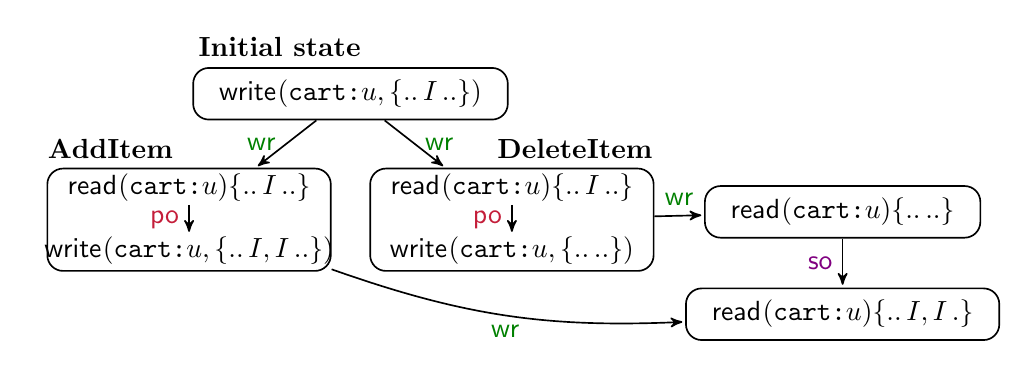
\begin{tikzpicture}[->,>=stealth',shorten >=1pt,auto,node distance=4cm,
			semithick, transform shape]
			\node (s11l) at (1.15, 2.1) {\textbf{Initial state}};
			\node[draw, rounded corners=2mm] (t0) at (2.05, 1.5) {\begin{tabular}{l} $\wrt{\texttt{cart:}u}{\{..\, I\, ..\}}$ \end{tabular}};
			\node[draw, rounded corners=2mm, minimum width=3.6cm, minimum height=1.3cm] (s1) at (0, -0.1) {};
			\node[style={inner sep=0,outer sep=0}] (s11) at (0, 0.3) {\begin{tabular}{l} $\rd{\texttt{cart:}u}{\{..\, I\, ..\}}$\end{tabular}};
			\node[style={inner sep=0,outer sep=0}] (s12) at (0, -0.5) {\begin{tabular}{l} $\wrt{\texttt{cart:}u}{\{..\, I,I\, ..\}}$ \end{tabular}};
			\node (s11l) at (-1, 0.8) {\textbf{AddItem}};
			\node[draw, rounded corners=2mm, minimum width=3.6cm, minimum height=1.3cm] (s2) at (4.1, -0.1) {};
			\node[style={inner sep=0,outer sep=0}] (s21) at (4.1, 0.3) {\begin{tabular}{l} $\rd{\texttt{cart:}u}{\{..\, I\, ..\}}$ \end{tabular}};
			\node[style={inner sep=0,outer sep=0}] (s22) at (4.1, -0.5) {\begin{tabular}{l} $\wrt{\texttt{cart:}u}{\{..\, ..\}}$ \end{tabular}};
			\node (s11l) at (4.9, 0.8) {\textbf{DeleteItem}};
			\node[draw, rounded corners=2mm] (r1) at (8.3, 0) {\begin{tabular}{l} $\rd{\texttt{cart:}u}{\{..\, ..\}}$ \end{tabular}};
			\node[draw, rounded corners=2mm] (r2) at (8.3, -1.3) {\begin{tabular}{l} $\rd{\texttt{cart:}u}{\{..\, I, I\, .\}}$ \end{tabular}};
			\path (s11) edge[left] node {$\po$} (s12);
			\path (s21) edge[left] node {$\po$} (s22);
			\path (t0) edge[left] node {$\wro$} (s1);
			\path (t0) edge[right] node {$\wro$} (s2);
			\path (r1) edge[left] node {$\so$} (r2);
			\path (s2) edge[above] node {$\wro$} (r1);
			\path (s1) edge[below,bend right=11] node {$\wro$} (r2);
			%    \path (t0) edge[red, right, bend left=20] node[pos=0.4,xshift=-1] {$\wro$} (s11);
			%    \path (t0) edge[red, left, bend right=20] node[pos=0.9,xshift=-1] {$\wro$} (s12);
		\end{tikzpicture}  
	}
	
	%  \begin{lstlisting}[xleftmargin=4mm,basicstyle=\ttfamily\footnotesize,escapeinside={(*}{*)},language=MyLang,morekeywords={Test,GetCart}]
	%Test: 
	%{ AddItem(I, u); GetCart(u); GetCart(u) } || DeleteItem(I, u)
	%		\end{lstlisting}
	\vspace{-2mm}
	\caption{A simple shopping cart service.}
	\label{fig:motiv}
	\vspace{-3mm}
\end{figure}

\textcolor{orange}{
%A weaker isolation level allows for more possible behaviors than stronger isolation levels. It is up to the developers then to ensure that their application can tolerate this larger set of behaviors. Unfortunately, weak isolation levels are hard to understand or reason about \cite{DBLP:conf/popl/BrutschyD0V17,adya-thesis} and resulting application bugs can cause loss of business \cite{acidrain}. Consider a simple shopping cart application, inspired from \citet{sivaramakrishnan2015declarative5}, that stores a per-client shopping cart in a key-value store (\textit{key} is the client ID and \textit{value} is a multi-set of items). \figref{motiv} shows procedures for adding an item to the cart (\texttt{AddItem}) and deleting \textit{all} instances of an item from the cart (\texttt{DeleteItem}). Each procedure executes in a transaction, represented by the calls to \texttt{begin} and \texttt{commit}. Suppose that initially, a user $u$ has a single instance of item $I$ in their cart. Then the user connects to the application via two different sessions (for instance, via two browser windows), adds $I$ in one session (\texttt{AddItem($I$, $u$)}) and deletes $I$ in the other session (\texttt{DeleteItem($I$, $u$)}). With serializability, the cart can either be left in the state $\{ I \}$ (delete happened first, followed by the add) or $\emptyset$ (delete happened second). However, with Causal Consistency (or Read Committed), it is possible that with two sequential reads of the shopping cart, the cart is empty in the first read (signaling that the delete has succeeded), but there are \textit{two} instances of $I$  in the second read! Such anomalies, of deleted items reappearing, have been noted in previous work \cite{decandia2007dynamo}. 
}

\paragraph{Testing storage-backed concurrent applications} Even in a serializable context, where the behaviors are limited, verifying a concurrent application is not a trivial task. Since decades researchers have been developed techniques for addressing this problem being the combined application of \textit{Stateless Model Checking} (SMC) and \textit{Dynamic Partial Order Reduction} (DPOR) algorithms the most promising approach. The former is a verification technique that explore all possible executions of a concurrent program without storing the set of states already visited, which avoids excessive memory consumption and improves the scalability factor of its implementations. The latter, on the other hand, refers to the establishment of some equivalence relation between different traces the program may execute. Thanks to these relations we can reduce the set of possible states and, therefore, notably decrease the time consumed.

In this paper we present STMC (Stateless Transactional Model-Checker), a DPOR algorithm for SMC storage-backed concurrent applications, where the multiple threads are only able to communicate between each other via the storage system and there is no transaction that is enable/disabled by any other. This algorithm is inspired in \textcolor{red}{cite Viktor's algorithm} and therefore our result is a \textit{sound}, \textit{complete} and \textit{optimal} algorithm which has a polynomial bound of memory on the program's size. Moreover, our approach is parametric on the storage model, supporting SER, $\CC$ and TRIVIAL models, and takes advantage on the write-read equivalence relation's flexibility to reduce the number of executed traces to those whose \textit{history} are different. \textcolor{blue}{Moreover, we present an alternative version of it focused on pure testing where some executions are discarded in order to, on average, detect earlier when some code is erroneous.}

To achieve this, we build upon prior work \---- most notably, \textcolor{red}{JPF} \---- and represent program executions as \textit{histories}. In summary, we make the following contributions:
\begin{itemize}
	\item We describe through a series of examples the huge difference between the multi-thread (MT) environment and the transactional one.
	\item We describe formally the working context and the notions that appears on it.
	\item We provide a series of algorithms which allow us to understand the resulting products.
	\item We formally prove that STMC is sound, complete and optimal.
	\item We implement a version of STMC, the unique tool at the moment of writing able to solve the problem addressed.
\end{itemize}

%SMC may allow a program to be verified employing polynomial memory and DPOR techniques may reduce exponentially the number of executing traces, but the task of obtaining an algorithm that explore all possible traces according to some semantics (\textit{completeness}) and nothing else (\textit{soundness}) without exploring redundant elements (\textit{optimality}) and using only a polynomial nu

%Thanks to the work of \textcolor{red}{cite things} complete, optimal algorithms that run in polynomial time 

%This paper addresses the problem of \textit{testing} code for correctness against weak behaviors: a developer should be able to write a test that runs their application and then asserts for correct behavior. The main difficulty with testing today is getting coverage of weak behaviors. Running against an actual production storage system is very likely to only result in serializable behaviors because of their optimized implementation. For instance, only 0.0004\% of all reads performed on Facebook's TAO storage system were not serializable \cite{facebook-consistency}. Emulators, offered by cloud providers for local development, on the other hand, do not support weaker isolation levels at all \cite{cosmosdb-local}. Another option, possible when the storage system is available open-source, is to set it up with a tool like Jepsen~\cite{jepsen} to inject noise (bring down replicas or delay packets on the network). This approach is unable to provide good coverage at the level of client operations \cite{clotho} (more details in \sectref{oltp}). Another line of work has focussed on finding anomalies by identifying non-serializable behavior (\sectref{related}). Anomalies, however, do not always correspond to bugs \cite{DBLP:conf/pldi/BrutschyD0V18,isodiff}; they may either not be important (e.g., gathering statistics in a non-serializable fashion may not impact application correctness) or may already be handled by the application (e.g., checking and deleting duplicate items).

\end{comment}
	%\section{Transactional environment}

\textcolor{red}{TODO: Add definitions of transactions and events}.

Why the transactional case is not trivially comparable to the multi-thread one? To answer this question let us dive in the previous literature. Strictly, an \textit{execution} is a total order between the instructions of a program given by the processor. However, this rigid definition does not take into account that some instructions can be reordered without affecting the program's semantics. The notion of \textit{history}, a graph whose vertices are instructions and whose edges are its relations, allow to express these similarities between executions. As those graphs are, essentially, due to the order between instructions in each thread joint with the write-read dependencies, one reasonable approach is translating the notion of history to the transactional case, where the only difference would be the vertices' type: instead of instructions now each vertex would be a whole transaction. This decision is reasonable as a MT history can be seen as a transactional history. The reverse, on the other hand, is not always true, and it is what enriches the environment: if in the MT context the vertices only could be a write node or a read node (depending on which instruction they were executing), in the transactional case each vertex can be a read-only, write-only or everything in between; as we can see in Figure~\ref{rc_example:1}.

\begin{figure}[H]
	
 \resizebox{.4\textwidth}{!}{
	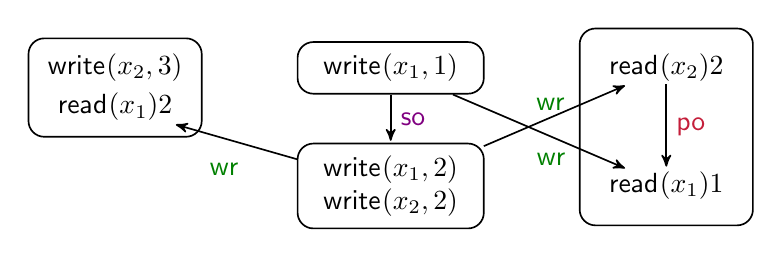
\begin{tikzpicture}[->,>=stealth',shorten >=1pt,auto,node distance=3cm,
		semithick, transform shape]
		\node[draw, rounded corners=2mm] (t1) at (0, 0) {\begin{tabular}{l} $\wrt{\key_1}{1}$ \end{tabular}};
		\node[draw, rounded corners=2mm,outer sep=0] (t2) at (0, -1.5) {\begin{tabular}{l} $\wrt{\key_1}{2}$ \\ $\wrt{\key_2}{2}$\end{tabular}};
		\node[draw, rounded corners=2mm, minimum width=2.2cm, minimum height=2.5cm] (t3) at (3.5, -0.75) {};
		\node[style={inner sep=0,outer sep=0}] (t3_1) at (3.5, 0) {\begin{tabular}{l} $\rd{\key_2}{2}$ \end{tabular}};
		\node[style={inner sep=0,outer sep=0}] (t3_2) at (3.5, -1.5) {\begin{tabular}{l} $\rd{\key_1}{1}$ \end{tabular}};
		\node[draw, rounded corners=2mm, minimum width=2.2cm, minimum height=1.25cm] (t4) at (-3.5, -0.25) {};
		\node[style={inner sep=0,outer sep=0}] (t4_1) at (-3.5, 0) {\begin{tabular}{l} $\wrt{\key_2}{3}$ \end{tabular}};
		\node[style={inner sep=0,outer sep=0}] (t4_2) at (-3.5, -0.5) {\begin{tabular}{l} $\rd{\key_1}{2}$ \end{tabular}};
		%\node[draw, rounded corners=2mm,outer sep=0] (t4) at (-3, 0) {\begin{tabular}{l} $\wrt{\key_1}{2}$ \\ $\rd{\key_2}{2}$\end{tabular}};
		% \path (t1) edge node {} (t3_2);
		% \path (t2) edge node {} (t3_1);
		\path (t1) edge node {$\so$} (t2);
		\path (t3_1) edge node {$\po$} (t3_2);
		\path (t1) edge[below] node[yshift=-4,xshift=4] {$\wro$} (t3_2);
		\path (t2) edge[below] node[yshift=-4,xshift=-4] {$\wro$} (t4_2);
		\path (t2) edge node[yshift=-2,xshift=7] {$\wro$} (t3_1);
	\end{tikzpicture}  
}

%\caption{$\mathsf{Read\ Committed}$ violation.}
%\label{rc_example:1}
\caption{A possible history that holds $\mathsf{Read\ Committed}$ axioms.}
\label{rc_example:1}
%\vspace{-3mm}
\end{figure}

Any deterministic algorithm that has as goal finding every possible history a MT-program may have (according to some memory model) has to execute step by step the ordered set of instructions, deciding for each one if there is any new non-explored history to take into account. When adding one new vertex and some edges to the graph, this new graph may be inconsistent according to the semantics of the model but may be mandatory to be explored to eventually produce all possible histories. \textcolor{red}{Example of this}. But it is clear that any non-naive algorithm whose aim is to be sound (i.e. not exploring histories that are not consistent) and complete (i.e. exploring every consistent history) will have to apply some strategy. Commonly, those are based on distinguish read and write vertices and applying one or another policy depending on the case.

It is clear that the immediate solution of adapting the same policies to transactions cannot be adapted. The second idea one could have thought about is applying those policies not to the transactions themselves but to the small instructions they execute. This idea, even if it is not perfect, handles part of the errors the most naive version had while assuming another hypothesis: the algorithm has access to every instruction a transaction can execute and can distinguish between them. This assumption is not minor, it heavily constraints the relation between different verifying tools, as the storage system verifier has to satisfy the algorithm information requirements.

\begin{figure}[H]
	
	\centering
	\begin{subfigure}{.29\textwidth}
		\resizebox{\textwidth}{!}{
			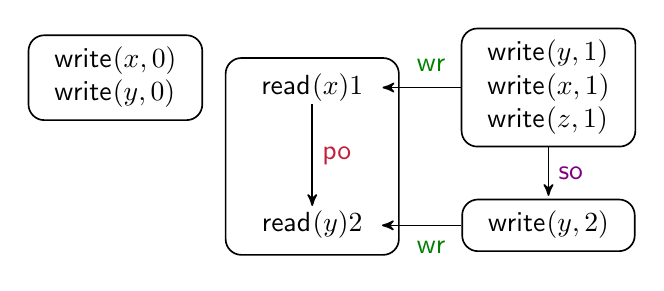
\begin{tikzpicture}[->,>=stealth',shorten >=1pt,auto,node distance=3cm,
				semithick, transform shape]
				\node[draw, rounded corners=2mm,outer sep=0] (t2) at (-2.5, 0.125) {\begin{tabular}{l} $\wrt{x}{0}$ \\ $\wrt{y}{0}$\end{tabular}};
				\node[draw, rounded corners=2mm, minimum width=2.2cm, minimum height=2.5cm] (t3) at (0, -0.875) {};
				\node[style={inner sep=0,outer sep=0}] (t3_1) at (0, 0) {\begin{tabular}{l} $\rd{x}{1}$ \end{tabular}};
				\node[style={inner sep=0,outer sep=0}] (t3_2) at (0, -1.75) {\begin{tabular}{l} $\rd{y}{2}$ \end{tabular}};
				\node[draw, rounded corners=2mm, minimum width=2.2cm, minimum height=1.25cm] (t4) at (3, -0) {\begin{tabular}{l} $\wrt{y}{1}$ \\ $\wrt{x}{1}$ \\
				$\wrt{z}{1}$ \end{tabular}};
				\node[draw, rounded corners=2mm] (t5) at (3, -1.75) {\begin{tabular}{l} $\wrt{y}{2}$ \end{tabular}};
				\path (t4) edge node {$\so$} (t5);
				\path (t3_1) edge node {$\po$} (t3_2);
				%\path (t1) edge[below] node[yshift=-4,xshift=-4] {$\wro$} (t3_2);
				%\path (t2) edge[below] node[yshift=-4,xshift=4] {$\wro$} (t4_2);
				\path (t4) edge[above] node[yshift=2,xshift=4] {$\wro$} (t3_1);
				\path (t5) edge[below] node[yshift=-2,xshift=4] {$\wro$} (t3_2);
			\end{tikzpicture}  
			
		}
		\caption{Objective trace.}
		\label{objective_trace:1}
	\end{subfigure}
	\hspace{.5cm}
	\centering
	\begin{subfigure}{.29\textwidth}
		\resizebox{\textwidth}{!}{
			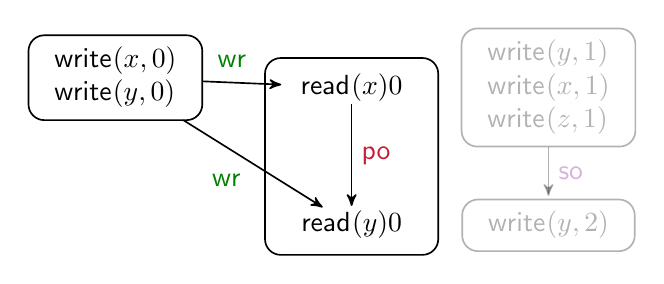
\begin{tikzpicture}[->,>=stealth',shorten >=1pt,auto,node distance=3cm,
				semithick, transform shape]
				\node[draw, rounded corners=2mm,outer sep=0] (t2) at (-3, 0.125) {\begin{tabular}{l} $\wrt{x}{0}$ \\ $\wrt{y}{0}$\end{tabular}};
				\node[draw, rounded corners=2mm, minimum width=2.2cm, minimum height=2.5cm] (t3) at (0, -0.875) {};
				\node[style={inner sep=0,outer sep=0}] (t3_1) at (0, 0) {\begin{tabular}{l} $\rd{x}{0}$ \end{tabular}};
				\node[style={inner sep=0,outer sep=0}] (t3_2) at (0, -1.75) {\begin{tabular}{l} $\rd{y}{0}$ \end{tabular}};
				\node[draw, rounded corners=2mm, minimum width=2.2cm, minimum height=1.25cm, opacity=0.3] (t4) at (2.5, -0) {
					\begin{tabular}{l} 
						$\wrt{y}{1}$ \\
						$\wrt{x}{1}$ \\
						$\wrt{z}{1}$
					 \end{tabular}};
				\node[draw, rounded corners=2mm, opacity=0.3] (t5) at (2.5, -1.75) {\begin{tabular}{l} $\wrt{y}{2}$ \end{tabular}};
				\path[opacity=0.3] (t4) edge node[opacity=0.3] {$\so$} (t5);
				\path (t3_1) edge node {$\po$} (t3_2);
				%\path (t1) edge[below] node[yshift=-4,xshift=-4] {$\wro$} (t3_2);
				%\path (t2) edge[below] node[yshift=-4,xshift=4] {$\wro$} (t4_2);
				\path (t2) edge[above] node[yshift=2,xshift=-4] {$\wro$} (t3_1);
				\path (t2) edge[below] node[yshift=0,xshift=-10] {$\wro$} (t3_2);
			\end{tikzpicture}  
			
		}
		\caption{Current trace.}
		\label{objective_trace:2}
	\end{subfigure}
	\hspace{.5cm}
	\centering
	\begin{subfigure}{.29\textwidth}
		\resizebox{\textwidth}{!}{
			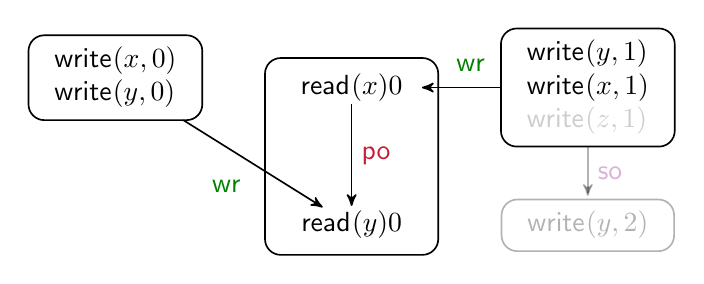
\begin{tikzpicture}[->,>=stealth',shorten >=1pt,auto,node distance=3cm,
				semithick, transform shape]
				\node[draw, rounded corners=2mm,outer sep=0] (t2) at (-3, 0.125) {\begin{tabular}{l} $\wrt{x}{0}$ \\ $\wrt{y}{0}$\end{tabular}};
				\node[draw, rounded corners=2mm, minimum width=2.2cm, minimum height=2.5cm] (t3) at (0, -0.875) {};
				\node[style={inner sep=0,outer sep=0}] (t3_1) at (0, 0) {\begin{tabular}{l} $\rd{x}{0}$ \end{tabular}};
				\node[style={inner sep=0,outer sep=0}] (t3_2) at (0, -1.75) {\begin{tabular}{l} $\rd{y}{0}$ \end{tabular}};
				\node[draw, rounded corners=2mm, minimum width=2.2cm, minimum height=1.25cm] (t4) at (3, -0) {\begin{tabular}{l} 
						$\wrt{y}{1}$ \\
						$\wrt{x}{1}$ \\
						{\pgfsetfillopacity{0.2}$\wrt{z}{1}$}
				\end{tabular}};
				\node[draw, rounded corners=2mm, opacity=0.3] (t5) at (3, -1.75) {\begin{tabular}{l} $\wrt{y}{2}$ \end{tabular}};
				\path[opacity=0.3] (t4) edge node[opacity=0.3] {$\so$} (t5);
				\path (t3_1) edge node {$\po$} (t3_2);
				%\path (t1) edge[below] node[yshift=-4,xshift=-4] {$\wro$} (t3_2);
				%\path (t2) edge[below] node[yshift=-4,xshift=4] {$\wro$} (t4_2);
				\path (t4) edge[above] node[yshift=2,xshift=4] {$\wro$} (t3_1);
				\path (t2) edge[below] node[yshift=-2,xshift=-10] {$\wro$} (t3_2);
			\end{tikzpicture}  
			
		}
		\caption{Incorrect trace.}
		\label{objective_trace:3}
	\end{subfigure}
	%\caption{Histories used to explain the axioms in Figure~\ref{consistency_defs}.}
	\label{counter_example:1}
	%\vspace{-3mm}
\end{figure}


Nevertheless, this idea is not enough to solve the problem: let's suppose that we have the situation \textcolor{red}{to be completed...}




%All the strategies have to face with the exponential number of different branches and the possible duplication on their generation

	%\section{A Stateless Transactional Model-Checker}

During this section we will present several approach for finding a deterministic transactional model checker and we will show why STMC is the best among them. Every approach would be, in some particular sense, incremental; starting from an empty history and ``upgrading'' it, adding in each step new events or relations. For any fixed program, we will assume that there is a finite number of transactions that no transaction enable/disable any other and that they are totally ordered by some relation $\ora$ called \textit{oracle order}. Therefore, combining $\ora$ and $\po$ we can also say that the oracle order also enforces a total order between the events. 

The naivest version for solving this problem would simply be executing every transaction and, afterwards, computing all possible graphs and discard those that are inconsistent. However, this exponential naive solution is very inefficient as it potentially compute an exponential number of histories that are inconsistent. Therefore, something more subtle has to be defined. The next idea one could think about would be executing the instructions according to $\ora$ step by step and only computing the possible graphs that this new event may produce. This reasonable refinement is based on the intuition that adding vertices/edges consistently to an already consistent history cannot produce an inconsistent result.

\begin{figure}[H]
	
	\centering
	\begin{subfigure}{.29\textwidth}
		\resizebox{\textwidth}{!}{
			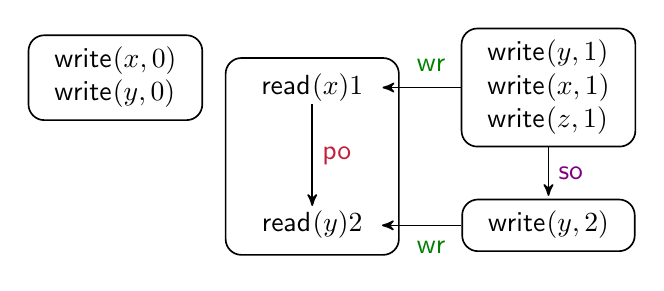
\begin{tikzpicture}[->,>=stealth',shorten >=1pt,auto,node distance=3cm,
				semithick, transform shape]
				\node[draw, rounded corners=2mm,outer sep=0] (t2) at (-2.5, 0.125) {\begin{tabular}{l} $\wrt{x}{0}$ \\ $\wrt{y}{0}$\end{tabular}};
				\node[draw, rounded corners=2mm, minimum width=2.2cm, minimum height=2.5cm] (t3) at (0, -0.875) {};
				\node[style={inner sep=0,outer sep=0}] (t3_1) at (0, 0) {\begin{tabular}{l} $\rd{x}{1}$ \end{tabular}};
				\node[style={inner sep=0,outer sep=0}] (t3_2) at (0, -1.75) {\begin{tabular}{l} $\rd{y}{2}$ \end{tabular}};
				\node[draw, rounded corners=2mm, minimum width=2.2cm, minimum height=1.25cm] (t4) at (3, -0) {\begin{tabular}{l} $\wrt{y}{1}$ \\ $\wrt{x}{1}$ \\
						$\wrt{z}{1}$ \end{tabular}};
				\node[draw, rounded corners=2mm] (t5) at (3, -1.75) {\begin{tabular}{l} $\wrt{y}{2}$ \end{tabular}};
				\path (t4) edge node {$\so$} (t5);
				\path (t3_1) edge node {$\po$} (t3_2);
				%\path (t1) edge[below] node[yshift=-4,xshift=-4] {$\wro$} (t3_2);
				%\path (t2) edge[below] node[yshift=-4,xshift=4] {$\wro$} (t4_2);
				\path (t4) edge[above] node[yshift=2,xshift=4] {$\wro$} (t3_1);
				\path (t5) edge[below] node[yshift=-2,xshift=4] {$\wro$} (t3_2);
			\end{tikzpicture}  
			
		}
		\caption{Target history.}
		\label{objective_trace:1}
	\end{subfigure}
	\hspace{.5cm}
	\centering
	\begin{subfigure}{.29\textwidth}
		\resizebox{\textwidth}{!}{
			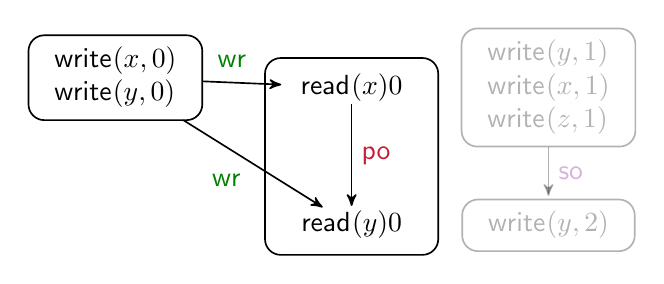
\begin{tikzpicture}[->,>=stealth',shorten >=1pt,auto,node distance=3cm,
				semithick, transform shape]
				\node[draw, rounded corners=2mm,outer sep=0] (t2) at (-3, 0.125) {\begin{tabular}{l} $\wrt{x}{0}$ \\ $\wrt{y}{0}$\end{tabular}};
				\node[draw, rounded corners=2mm, minimum width=2.2cm, minimum height=2.5cm] (t3) at (0, -0.875) {};
				\node[style={inner sep=0,outer sep=0}] (t3_1) at (0, 0) {\begin{tabular}{l} $\rd{x}{0}$ \end{tabular}};
				\node[style={inner sep=0,outer sep=0}] (t3_2) at (0, -1.75) {\begin{tabular}{l} $\rd{y}{0}$ \end{tabular}};
				\node[draw, rounded corners=2mm, minimum width=2.2cm, minimum height=1.25cm, opacity=0.3] (t4) at (2.5, -0) {
					\begin{tabular}{l} 
						$\wrt{y}{1}$ \\
						$\wrt{x}{1}$ \\
						$\wrt{z}{1}$
				\end{tabular}};
				\node[draw, rounded corners=2mm, opacity=0.3] (t5) at (2.5, -1.75) {\begin{tabular}{l} $\wrt{y}{2}$ \end{tabular}};
				\path[opacity=0.3] (t4) edge node[opacity=0.3] {$\so$} (t5);
				\path (t3_1) edge node {$\po$} (t3_2);
				%\path (t1) edge[below] node[yshift=-4,xshift=-4] {$\wro$} (t3_2);
				%\path (t2) edge[below] node[yshift=-4,xshift=4] {$\wro$} (t4_2);
				\path (t2) edge[above] node[yshift=2,xshift=-4] {$\wro$} (t3_1);
				\path (t2) edge[below] node[yshift=0,xshift=-10] {$\wro$} (t3_2);
			\end{tikzpicture}  
			
		}
		\caption{Current history.}
		\label{objective_trace:2}
	\end{subfigure}
	\hspace{.5cm}
	\centering
	\begin{subfigure}{.29\textwidth}
		\resizebox{\textwidth}{!}{
			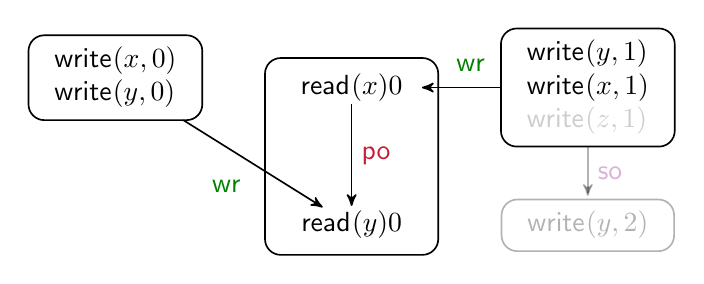
\begin{tikzpicture}[->,>=stealth',shorten >=1pt,auto,node distance=3cm,
				semithick, transform shape]
				\node[draw, rounded corners=2mm,outer sep=0] (t2) at (-3, 0.125) {\begin{tabular}{l} $\wrt{x}{0}$ \\ $\wrt{y}{0}$\end{tabular}};
				\node[draw, rounded corners=2mm, minimum width=2.2cm, minimum height=2.5cm] (t3) at (0, -0.875) {};
				\node[style={inner sep=0,outer sep=0}] (t3_1) at (0, 0) {\begin{tabular}{l} $\rd{x}{0}$ \end{tabular}};
				\node[style={inner sep=0,outer sep=0}] (t3_2) at (0, -1.75) {\begin{tabular}{l} $\rd{y}{0}$ \end{tabular}};
				\node[draw, rounded corners=2mm, minimum width=2.2cm, minimum height=1.25cm] (t4) at (3, -0) {\begin{tabular}{l} 
						$\wrt{y}{1}$ \\
						$\wrt{x}{1}$ \\
						{\pgfsetfillopacity{0.2}$\wrt{z}{1}$}
				\end{tabular}};
				\node[draw, rounded corners=2mm, opacity=0.3] (t5) at (3, -1.75) {\begin{tabular}{l} $\wrt{y}{2}$ \end{tabular}};
				\path[opacity=0.3] (t4) edge node[opacity=0.3] {$\so$} (t5);
				\path (t3_1) edge node {$\po$} (t3_2);
				%\path (t1) edge[below] node[yshift=-4,xshift=-4] {$\wro$} (t3_2);
				%\path (t2) edge[below] node[yshift=-4,xshift=4] {$\wro$} (t4_2);
				\path (t4) edge[above] node[yshift=2,xshift=4] {$\wro$} (t3_1);
				\path (t2) edge[below] node[yshift=-2,xshift=-10] {$\wro$} (t3_2);
			\end{tikzpicture}  
			
		}
		\caption{Inconsistent history.}
		\label{objective_trace:3}
	\end{subfigure}
	\caption{The history in \ref{objective_trace:1} cannot be obtained from \ref{objective_trace:2} with a naive approach.}
	\label{fig:objective_trace_counterexample}
	%\vspace{-3mm}
\end{figure}

Is the intuition beneath this approach enough? Let's suppose that a program runs over a serializable (SER) storage system. One of its possible histories can be seen in Figure~\ref{objective_trace:1}, history that we will call target. One possible total order of the transactions in this program could be order them from left to right, top to bottom; let's suppose this order is $\ora$. Following this order, this algorithm would have executed the first two transactions obtaining the history seen in Figure~\ref{objective_trace:2}. The 

%this problem would simply be, each time one event is added to a history, every other possible graph that can be deduce from it changing some $\wr$-edges is computed. This recursive and simple version is clearly complete and sound, but it is clear non-optimal, as adding one event may lead to several graphs already explored in some other branches. For example, the histories $h_1$ and $h_2$ presented in Figure~\ref{fig:naive} would produce each one the four alternative graphs that can arise after introducing the light gray transaction $\wrt{y}{2}$. 

\begin{comment}

\begin{figure}[H]
\centering
\begin{subfigure}[b]{\linewidth}
\centering
\begin{minipage}[b]{0.4\textwidth}
\resizebox{\textwidth}{!}{
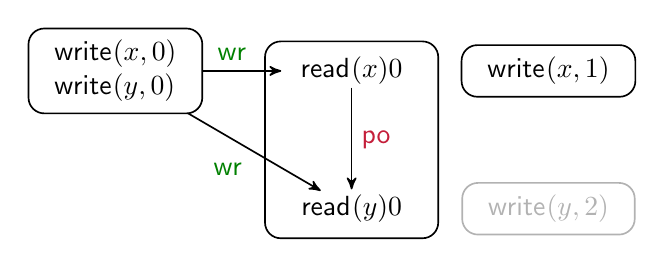
\begin{tikzpicture}[->,>=stealth',shorten >=1pt,auto,node distance=3cm,
semithick, transform shape]
\node[draw, rounded corners=2mm,outer sep=0] (t2) at (-3, -0) {\begin{tabular}{l} $\wrt{x}{0}$ \\ $\wrt{y}{0}$\end{tabular}};
\node[draw, rounded corners=2mm, minimum width=2.2cm, minimum height=2.5cm] (t3) at (0, -0.875) {};
\node[style={inner sep=0,outer sep=0}] (t3_1) at (0, 0) {\begin{tabular}{l} $\rd{x}{0}$ \end{tabular}};
\node[style={inner sep=0,outer sep=0}] (t3_2) at (0, -1.75) {\begin{tabular}{l} $\rd{y}{0}$ \end{tabular}};
\node[draw, rounded corners=2mm] (t4) at (2.5, -0) {
\begin{tabular}{l} 
$\wrt{x}{1}$
\end{tabular}};
\node[draw, rounded corners=2mm, opacity=0.3] (t5) at (2.5, -1.75) {\begin{tabular}{l} $\wrt{y}{2}$ \end{tabular}};
%\path[] (t4) edge node[] {$\so$} (t5);
\path (t3_1) edge node {$\po$} (t3_2);
%\path (t1) edge[below] node[yshift=-4,xshift=-4] {$\wro$} (t3_2);
%\path (t2) edge[below] node[yshift=-4,xshift=4] {$\wro$} (t4_2);
\path (t2) edge[above] node[yshift=0,xshift=-4] {$\wro$} (t3_1);
\path (t2) edge[below] node[yshift=0,xshift=-10] {$\wro$} (t3_2);
\end{tikzpicture}  
}
\caption{History $1$.}
\end{minipage}
\hspace{.5cm}
\begin{minipage}[b]{0.4\textwidth}
\resizebox{\textwidth}{!}{
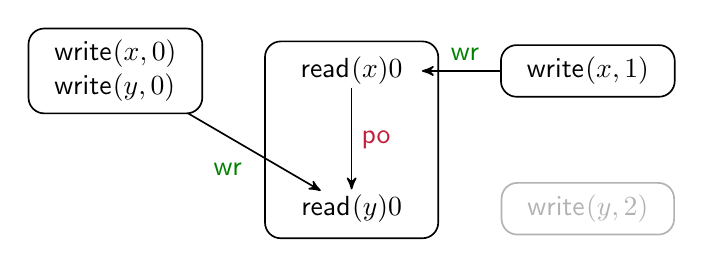
\begin{tikzpicture}[->,>=stealth',shorten >=1pt,auto,node distance=3cm,
semithick, transform shape]
\node[draw, rounded corners=2mm,outer sep=0] (t2) at (-3, -0) {\begin{tabular}{l} $\wrt{x}{0}$ \\ $\wrt{y}{0}$\end{tabular}};
\node[draw, rounded corners=2mm, minimum width=2.2cm, minimum height=2.5cm] (t3) at (0, -0.875) {};
\node[style={inner sep=0,outer sep=0}] (t3_1) at (0, 0) {\begin{tabular}{l} $\rd{x}{0}$ \end{tabular}};
\node[style={inner sep=0,outer sep=0}] (t3_2) at (0, -1.75) {\begin{tabular}{l} $\rd{y}{0}$ \end{tabular}};
\node[draw, rounded corners=2mm] (t4) at (3, -0) {
\begin{tabular}{l} 
$\wrt{x}{1}$
\end{tabular}};
\node[draw, rounded corners=2mm, opacity=0.3] (t5) at (3, -1.75) {\begin{tabular}{l} $\wrt{y}{2}$ \end{tabular}};
%\path[] (t4) edge node[] {$\so$} (t5);
\path (t3_1) edge node {$\po$} (t3_2);
%\path (t1) edge[below] node[yshift=-4,xshift=-4] {$\wro$} (t3_2);
%\path (t2) edge[below] node[yshift=-4,xshift=4] {$\wro$} (t4_2);
\path (t4) edge[above] node[yshift=0,xshift=2] {$\wro$} (t3_1);
\path (t2) edge[below] node[yshift=0,xshift=-10] {$\wro$} (t3_2);
\end{tikzpicture}  
}
\caption{History $2$.}
\end{minipage}
\end{subfigure}
\caption{Two histories that naively produce redundancies}
\label{fig:naive}
\end{figure}




\begin{figure}[H]
	    \centering
	\begin{subfigure}[b]{\linewidth}
		\centering
		\begin{minipage}[b]{0.4\textwidth}
			\resizebox{\textwidth}{!}{
			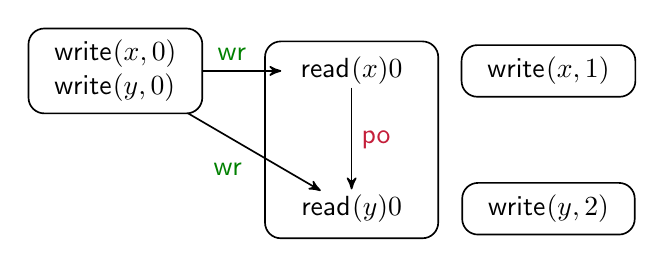
\begin{tikzpicture}[->,>=stealth',shorten >=1pt,auto,node distance=3cm,
				semithick, transform shape]
				\node[draw, rounded corners=2mm,outer sep=0] (t2) at (-3, -0) {\begin{tabular}{l} $\wrt{x}{0}$ \\ $\wrt{y}{0}$\end{tabular}};
				\node[draw, rounded corners=2mm, minimum width=2.2cm, minimum height=2.5cm] (t3) at (0, -0.875) {};
				\node[style={inner sep=0,outer sep=0}] (t3_1) at (0, 0) {\begin{tabular}{l} $\rd{x}{0}$ \end{tabular}};
				\node[style={inner sep=0,outer sep=0}] (t3_2) at (0, -1.75) {\begin{tabular}{l} $\rd{y}{0}$ \end{tabular}};
				\node[draw, rounded corners=2mm] (t4) at (2.5, -0) {
					\begin{tabular}{l} 
						$\wrt{x}{1}$
				\end{tabular}};
				\node[draw, rounded corners=2mm] (t5) at (2.5, -1.75) {\begin{tabular}{l} $\wrt{y}{2}$ \end{tabular}};
				%\path[] (t4) edge node[] {$\so$} (t5);
				\path (t3_1) edge node {$\po$} (t3_2);
				%\path (t1) edge[below] node[yshift=-4,xshift=-4] {$\wro$} (t3_2);
				%\path (t2) edge[below] node[yshift=-4,xshift=4] {$\wro$} (t4_2);
				\path (t2) edge[above] node[yshift=0,xshift=-4] {$\wro$} (t3_1);
				\path (t2) edge[below] node[yshift=0,xshift=-10] {$\wro$} (t3_2);
			\end{tikzpicture}  
			}
			\caption{History $1$.}
		\end{minipage}
		\hspace{.5cm}
		\begin{minipage}[b]{0.4\textwidth}
			\resizebox{\textwidth}{!}{
				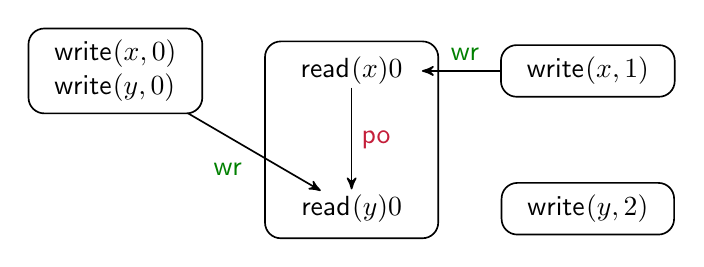
\begin{tikzpicture}[->,>=stealth',shorten >=1pt,auto,node distance=3cm,
					semithick, transform shape]
					\node[draw, rounded corners=2mm,outer sep=0] (t2) at (-3, -0) {\begin{tabular}{l} $\wrt{x}{0}$ \\ $\wrt{y}{0}$\end{tabular}};
					\node[draw, rounded corners=2mm, minimum width=2.2cm, minimum height=2.5cm] (t3) at (0, -0.875) {};
					\node[style={inner sep=0,outer sep=0}] (t3_1) at (0, 0) {\begin{tabular}{l} $\rd{x}{0}$ \end{tabular}};
					\node[style={inner sep=0,outer sep=0}] (t3_2) at (0, -1.75) {\begin{tabular}{l} $\rd{y}{0}$ \end{tabular}};
					\node[draw, rounded corners=2mm] (t4) at (3, -0) {
						\begin{tabular}{l} 
							$\wrt{x}{1}$
					\end{tabular}};
					\node[draw, rounded corners=2mm] (t5) at (3, -1.75) {\begin{tabular}{l} $\wrt{y}{2}$ \end{tabular}};
					%\path[] (t4) edge node[] {$\so$} (t5);
					\path (t3_1) edge node {$\po$} (t3_2);
					%\path (t1) edge[below] node[yshift=-4,xshift=-4] {$\wro$} (t3_2);
					%\path (t2) edge[below] node[yshift=-4,xshift=4] {$\wro$} (t4_2);
					\path (t4) edge[above] node[yshift=0,xshift=2] {$\wro$} (t3_1);
					\path (t2) edge[below] node[yshift=0,xshift=-10] {$\wro$} (t3_2);
				\end{tikzpicture}  
			}
			\caption{History $2$.}
		\end{minipage}
	\end{subfigure}
	\hspace{.5cm}
	\begin{subfigure}[b]{\linewidth}
		\centering
		\begin{minipage}[b]{0.4\textwidth}
			\resizebox{\textwidth}{!}{
				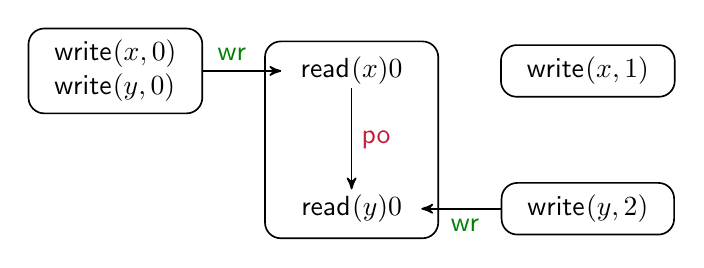
\begin{tikzpicture}[->,>=stealth',shorten >=1pt,auto,node distance=3cm,
					semithick, transform shape]
					\node[draw, rounded corners=2mm,outer sep=0] (t2) at (-3, -0) {\begin{tabular}{l} $\wrt{x}{0}$ \\ $\wrt{y}{0}$\end{tabular}};
					\node[draw, rounded corners=2mm, minimum width=2.2cm, minimum height=2.5cm] (t3) at (0, -0.875) {};
					\node[style={inner sep=0,outer sep=0}] (t3_1) at (0, 0) {\begin{tabular}{l} $\rd{x}{0}$ \end{tabular}};
					\node[style={inner sep=0,outer sep=0}] (t3_2) at (0, -1.75) {\begin{tabular}{l} $\rd{y}{0}$ \end{tabular}};
					\node[draw, rounded corners=2mm] (t4) at (3, -0) {
						\begin{tabular}{l} 
							$\wrt{x}{1}$
					\end{tabular}};
					\node[draw, rounded corners=2mm] (t5) at (3, -1.75) {\begin{tabular}{l} $\wrt{y}{2}$ \end{tabular}};
					%\path[] (t4) edge node[] {$\so$} (t5);
					\path (t3_1) edge node {$\po$} (t3_2);
					%\path (t1) edge[below] node[yshift=-4,xshift=-4] {$\wro$} (t3_2);
					%\path (t2) edge[below] node[yshift=-4,xshift=4] {$\wro$} (t4_2);
					\path (t2) edge[above] node[yshift=0,xshift=-4] {$\wro$} (t3_1);
					\path (t5) edge[below] node[yshift=0,xshift=2] {$\wro$} (t3_2);
				\end{tikzpicture}  
			}
			\caption{History $3$.}
		\end{minipage}
		\hspace{.5cm}
		\begin{minipage}[b]{0.4\textwidth}
			\resizebox{\textwidth}{!}{
				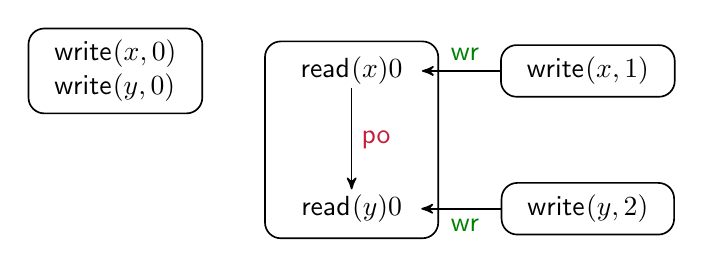
\begin{tikzpicture}[->,>=stealth',shorten >=1pt,auto,node distance=3cm,
					semithick, transform shape]
					\node[draw, rounded corners=2mm,outer sep=0] (t2) at (-3, -0) {\begin{tabular}{l} $\wrt{x}{0}$ \\ $\wrt{y}{0}$\end{tabular}};
					\node[draw, rounded corners=2mm, minimum width=2.2cm, minimum height=2.5cm] (t3) at (0, -0.875) {};
					\node[style={inner sep=0,outer sep=0}] (t3_1) at (0, 0) {\begin{tabular}{l} $\rd{x}{0}$ \end{tabular}};
					\node[style={inner sep=0,outer sep=0}] (t3_2) at (0, -1.75) {\begin{tabular}{l} $\rd{y}{0}$ \end{tabular}};
					\node[draw, rounded corners=2mm] (t4) at (3, -0) {
						\begin{tabular}{l} 
							$\wrt{x}{1}$
					\end{tabular}};
					\node[draw, rounded corners=2mm] (t5) at (3, -1.75) {\begin{tabular}{l} $\wrt{y}{2}$ \end{tabular}};
					%\path[] (t4) edge node[] {$\so$} (t5);
					\path (t3_1) edge node {$\po$} (t3_2);
					%\path (t1) edge[below] node[yshift=-4,xshift=-4] {$\wro$} (t3_2);
					%\path (t2) edge[below] node[yshift=-4,xshift=4] {$\wro$} (t4_2);
					\path (t4) edge[above] node[yshift=0,xshift=2] {$\wro$} (t3_1);
					\path (t5) edge[below] node[yshift=0,xshift=2] {$\wro$} (t3_2);
				\end{tikzpicture}  
			}
			\caption{History $4$.}
		\end{minipage}
	\end{subfigure}
\caption{All possible complete histories.}
\label{fig:all_histories}
\end{figure}

\begin{figure}[H]
	


\centering
\begin{subfigure}{.35\textwidth}
	
	\resizebox{\textwidth}{!}{
		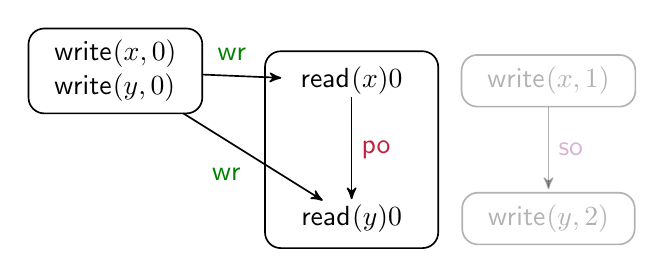
\begin{tikzpicture}[->,>=stealth',shorten >=1pt,auto,node distance=3cm,
			semithick, transform shape]
			\node[draw, rounded corners=2mm,outer sep=0] (t2) at (-3, 0.125) {\begin{tabular}{l} $\wrt{x}{0}$ \\ $\wrt{y}{0}$\end{tabular}};
			\node[draw, rounded corners=2mm, minimum width=2.2cm, minimum height=2.5cm] (t3) at (0, -0.875) {};
			\node[style={inner sep=0,outer sep=0}] (t3_1) at (0, 0) {\begin{tabular}{l} $\rd{x}{0}$ \end{tabular}};
			\node[style={inner sep=0,outer sep=0}] (t3_2) at (0, -1.75) {\begin{tabular}{l} $\rd{y}{0}$ \end{tabular}};
			\node[draw, rounded corners=2mm, opacity=0.3] (t4) at (2.5, -0) {
				\begin{tabular}{l} 
					$\wrt{x}{1}$
			\end{tabular}};
			\node[draw, rounded corners=2mm, opacity=0.3] (t5) at (2.5, -1.75) {\begin{tabular}{l} $\wrt{y}{2}$ \end{tabular}};
			\path[opacity=0.3] (t4) edge node[opacity=0.3] {$\so$} (t5);
			\path (t3_1) edge node {$\po$} (t3_2);
			%\path (t1) edge[below] node[yshift=-4,xshift=-4] {$\wro$} (t3_2);
			%\path (t2) edge[below] node[yshift=-4,xshift=4] {$\wro$} (t4_2);
			\path (t2) edge[above] node[yshift=2,xshift=-4] {$\wro$} (t3_1);
			\path (t2) edge[below] node[yshift=0,xshift=-10] {$\wro$} (t3_2);
		\end{tikzpicture}  
	}
	\caption{Initial history.}
\end{subfigure}
\hspace{.5cm}
\centering
\begin{subfigure}{.35\textwidth}
	\resizebox{\textwidth}{!}{
		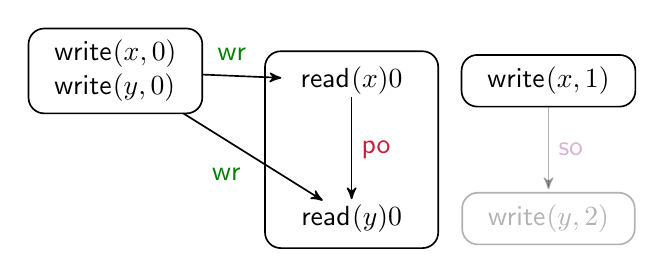
\begin{tikzpicture}[->,>=stealth',shorten >=1pt,auto,node distance=3cm,
			semithick, transform shape]
			\node[draw, rounded corners=2mm,outer sep=0] (t2) at (-3, 0.125) {\begin{tabular}{l} $\wrt{x}{0}$ \\ $\wrt{y}{0}$\end{tabular}};
			\node[draw, rounded corners=2mm, minimum width=2.2cm, minimum height=2.5cm] (t3) at (0, -0.875) {};
			\node[style={inner sep=0,outer sep=0}] (t3_1) at (0, 0) {\begin{tabular}{l} $\rd{x}{0}$ \end{tabular}};
			\node[style={inner sep=0,outer sep=0}] (t3_2) at (0, -1.75) {\begin{tabular}{l} $\rd{y}{0}$ \end{tabular}};
			\node[draw, rounded corners=2mm] (t4) at (2.5, -0) {
				\begin{tabular}{l} 
					$\wrt{x}{1}$
			\end{tabular}};
			\node[draw, rounded corners=2mm, opacity=0.3] (t5) at (2.5, -1.75) {\begin{tabular}{l} $\wrt{y}{2}$ \end{tabular}};
			\path[opacity=0.3] (t4) edge node[opacity=0.3] {$\so$} (t5);
			\path (t3_1) edge node {$\po$} (t3_2);
			%\path (t1) edge[below] node[yshift=-4,xshift=-4] {$\wro$} (t3_2);
			%\path (t2) edge[below] node[yshift=-4,xshift=4] {$\wro$} (t4_2);
			\path (t2) edge[above] node[yshift=2,xshift=-4] {$\wro$} (t3_1);
			\path (t2) edge[below] node[yshift=0,xshift=-10] {$\wro$} (t3_2);
		\end{tikzpicture}  
		
	}
	\caption{Incorrect trace.}
	\label{objective_trace:3}
\end{subfigure}
\hspace{.5cm}
\centering
\begin{subfigure}{.35\textwidth}
	\resizebox{\textwidth}{!}{
		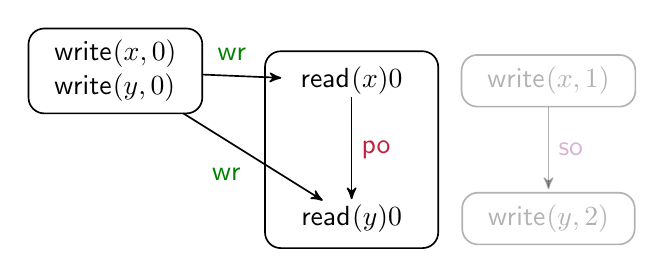
\begin{tikzpicture}[->,>=stealth',shorten >=1pt,auto,node distance=3cm,
			semithick, transform shape]
			\node[draw, rounded corners=2mm,outer sep=0] (t2) at (-3, 0.125) {\begin{tabular}{l} $\wrt{x}{0}$ \\ $\wrt{y}{0}$\end{tabular}};
			\node[draw, rounded corners=2mm, minimum width=2.2cm, minimum height=2.5cm] (t3) at (0, -0.875) {};
			\node[style={inner sep=0,outer sep=0}] (t3_1) at (0, 0) {\begin{tabular}{l} $\rd{x}{0}$ \end{tabular}};
			\node[style={inner sep=0,outer sep=0}] (t3_2) at (0, -1.75) {\begin{tabular}{l} $\rd{y}{0}$ \end{tabular}};
			\node[draw, rounded corners=2mm, opacity=0.3] (t4) at (2.5, -0) {
				\begin{tabular}{l} 
					$\wrt{x}{1}$
			\end{tabular}};
			\node[draw, rounded corners=2mm, opacity=0.3] (t5) at (2.5, -1.75) {\begin{tabular}{l} $\wrt{y}{2}$ \end{tabular}};
			\path[opacity=0.3] (t4) edge node[opacity=0.3] {$\so$} (t5);
			\path (t3_1) edge node {$\po$} (t3_2);
			%\path (t1) edge[below] node[yshift=-4,xshift=-4] {$\wro$} (t3_2);
			%\path (t2) edge[below] node[yshift=-4,xshift=4] {$\wro$} (t4_2);
			\path (t2) edge[above] node[yshift=2,xshift=-4] {$\wro$} (t3_1);
			\path (t2) edge[below] node[yshift=0,xshift=-10] {$\wro$} (t3_2);
		\end{tikzpicture}  
	}
	\caption{Initial history.}
\end{subfigure}
\hspace{.5cm}
\centering
\begin{subfigure}{.35\textwidth}
	\resizebox{\textwidth}{!}{
		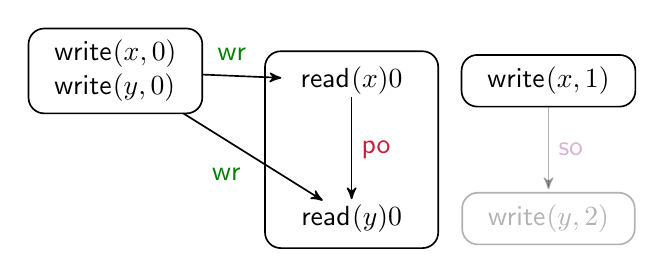
\begin{tikzpicture}[->,>=stealth',shorten >=1pt,auto,node distance=3cm,
			semithick, transform shape]
			\node[draw, rounded corners=2mm,outer sep=0] (t2) at (-3, 0.125) {\begin{tabular}{l} $\wrt{x}{0}$ \\ $\wrt{y}{0}$\end{tabular}};
			\node[draw, rounded corners=2mm, minimum width=2.2cm, minimum height=2.5cm] (t3) at (0, -0.875) {};
			\node[style={inner sep=0,outer sep=0}] (t3_1) at (0, 0) {\begin{tabular}{l} $\rd{x}{0}$ \end{tabular}};
			\node[style={inner sep=0,outer sep=0}] (t3_2) at (0, -1.75) {\begin{tabular}{l} $\rd{y}{0}$ \end{tabular}};
			\node[draw, rounded corners=2mm] (t4) at (2.5, -0) {
				\begin{tabular}{l} 
					$\wrt{x}{1}$
			\end{tabular}};
			\node[draw, rounded corners=2mm, opacity=0.3] (t5) at (2.5, -1.75) {\begin{tabular}{l} $\wrt{y}{2}$ \end{tabular}};
			\path[opacity=0.3] (t4) edge node[opacity=0.3] {$\so$} (t5);
			\path (t3_1) edge node {$\po$} (t3_2);
			%\path (t1) edge[below] node[yshift=-4,xshift=-4] {$\wro$} (t3_2);
			%\path (t2) edge[below] node[yshift=-4,xshift=4] {$\wro$} (t4_2);
			\path (t2) edge[above] node[yshift=2,xshift=-4] {$\wro$} (t3_1);
			\path (t2) edge[below] node[yshift=0,xshift=-10] {$\wro$} (t3_2);
		\end{tikzpicture}  
		
	}
	\caption{Incorrect trace.}
	\label{objective_trace:3}
\end{subfigure}
	%\caption{Histories used to explain the axioms in Figure~\ref{consistency_defs}.}
	\label{counter_example:1}
	%\vspace{-3mm}
\end{figure}

\end{comment}
	%!TEX root = main.tex
\section{Transactional Programs}\label{sec:prelims}

\newcommand{\icommit}{\mathtt{commit}}

\subsection{Program Syntax}

\begin{figure}
\small
\begin{align*}
\key\in \Vars\quad \xvar\in\LVars
\end{align*}
\begin{minipage}[t]{.4\textwidth}
\begin{align*}
\mathsf{Prog} &  \eqdef  \mathsf{Sess} \ \mid\  \mathsf{Sess}\,||\,\mathsf{Prog} \\
\mathsf{Sess} & \eqdef  \mathsf{Trans} \ \mid\  \mathsf{Trans}; \mathsf{Sess} \\
\mathsf{Trans} & \eqdef  \ibegin; \mathsf{Body}; \icommit 
\end{align*}
\end{minipage}
\begin{minipage}[t]{.4\textwidth}
\begin{align*}
\mathsf{Body} & \eqdef  \mathsf{Instr} \ \mid\  \mathsf{Instr}; \mathsf{Body} \\
\mathsf{Instr} & \eqdef  \mathsf{InstrDB} \ \mid\  a := e \mid\ \iif{\phi(\vec{a})}{\mathsf{Instr}} \\
\mathsf{InstrDB} & \eqdef \xvar := \iread(\key)  \ \mid\  \iwrite(\key,\xvar) 
%\mathsf{Local} & \eqdef  x := e
\end{align*}
\end{minipage}
%\vspace{-6mm}
\caption{Program syntax. The set of global variables is denoted by $\Vars$ while $\LVars$ denotes the set of local variables.
We use $\phi$ to denote Boolean expressions over local variables, and $e$ to denote expressions over local variables interpreted as values. We use $\vec{\cdot}$ to denote vectors of elements.}
\label{fig:syntax}
%\vspace{-4mm}
\end{figure}

Figure~\ref{fig:syntax} lists the definition of a simple programming language
that we use to represent applications running on top of a database. A program is a set of \emph{sessions} running in parallel, each
session being composed of a sequence of \emph{transactions}. Each transaction is
delimited by $\ibegin$ and $\icommit$ instructions, and its body contains instructions that access the
database and manipulate a set $\LVars$ of local variables.\footnote{For simplicity, we
assume that all the transactions in the program commit. Aborted transactions can
be ignored when reasoning about safety because their effects should be invisible
to other transactions.} We use symbols 
$a$, $b$, etc. to denote elements of $\LVars$.

For simplicity, we abstract the database state as a valuation to a set $\Vars$ of \emph{global} variables\footnote{In the context of a relational database, global variables correspond to fields/rows of a table while in the context of a key-value store, they correspond to keys.}, ranged over using $x$, $y$, etc. The instructions accessing the database correspond to reading the value of a global variable and storing it into a local variable $a$ ($a := \iread(x)$) , writing the value of a local variable $a$ to a global variable $x$ ($\iwrite(x,a)$), or an assignment to a local variable $a$ ($a := e$). The set of values of global or local variables is denoted by $\Vals$. Assignments to local variables use expressions $e$ over local variables, which are interpreted as values and whose syntax is left unspecified. Each of these instructions can be guarded by a Boolean condition $\phi(\vec{a})$ over a set of local variables $\vec{a}$ (their syntax is not important). Our results assume bounded programs, as usual in SMC algorithms, and therefore, we omit other constructs like $\mathtt{while}$ loops.
%Other constructs like $\mathtt{while}$ loops can be defined in a similar way. 
%Let $\KVProgs$ denote the set of programs where a transaction body can contain only such instructions.

\subsection{Isolation Levels}

We present the axiomatic framework introduced
by \citet{DBLP:journals/pacmpl/BiswasE19} for defining isolation levels\footnote{Isolation levels are called consistency models by \citet{DBLP:journals/pacmpl/BiswasE19}.}.
Isolation levels are defined as logical constraints, called \emph{axioms}, over \emph{histories}, which are an abstract representation of the interaction between a program and the database in a concrete execution. 
% that record the sequence of reads and writes executed in each transaction, the order between transactions in each session, and a write-read relation (also called read-from) that ``justifies'' read values by associating each read to a write that wrote the value returned by the read.

%TODO SOME INTRO EXPLAINING THAT ISOLATION LEVELS ARE DEFINED AS AXIOMS OVER HISTORIES, WHICH REPRESENT THE INTERACTION BETWEEN A PROGRAM AND A STORE. 

\subsubsection{Histories}

Programs interact with a database by issuing transactions formed of $\ibegin$, $\iend$, $\textsf{read}$ and $\textsf{write}$ instructions. The effect of executing one such instruction is represented using an \emph{event} $\langle e, \mathit{type} \rangle$ where $e$ is an \textit{identifier} and $\mathit{type} $ is a \textit{type}. There are four types of events: $\ebegin$, $\eend$, $\erd{x}$ for reading the global variable $x$, and $\ewrt{x,v}$ for writing value $v$ to global variable $x$. The set of events is denoted by $\Events$.
For a read/write event $e$, we use $\mathit{var}(e)$ to denote the variable $x$. % and $\mathit{val}(e)$ the value $v$.

A \emph{transaction log} $\tup{t,E, \po_t}$ is an identifier $t$ and a finite set of events $E$ along with a strict total order $\po_t$ on $E$, called \emph{program order}.
%$T$  is a finite sequence of events ordered by a strict total order $\po_T$ called \emph{program order}. 
The minimal element of $\po_t$ is a $\ebegin$ event. A transaction log without a $\eend$ event is called \emph{pending}. Otherwise, it is called \emph{complete}. If the $\eend$ event occurs, then it is maximal in $\po_t$. The set $E$ of events in a transaction log $t$ is denoted by $\events{t}$.

The program order $\po_t$ represents the order between instructions in the body of a transaction. We assume that each transaction log is well-formed in the sense that if a read of a global variable $x$ is preceded by a write to $x$ in $\po_t$, then it should return the value written by the last write to $x$ before the read (w.r.t. $\po_t$). This property is implicit in the definition of every isolation level that we are aware of. For simplicity, we may use the term \emph{transaction} instead of transaction log. %The  set of all transaction logs is denoted by $\mathsf{Tlogs}$.

%For every transaction $T$, we denote $\po_T$ the total order existing between the events in $T$.
%During the whole paper we will assume that every pair of transactions are disjoint and that both $\mathcal{E}$ and $\mathcal{T}$ are finite. Therefore, we denote the function $tr: \mathcal{E} \to \mathcal{T}$ that associates every event to the unique transaction it belongs to. %Moreover, we will assume there is a special transaction called \callout{initial} that contains exactly one write event for every possible variable.

The set of $\erd{x}$ events in a transaction log $t$ that are \textit{not} preceded by a write to $x$ in $\po_t$, for some $x$, is denoted by $\readOp{t}$. As mentioned above, the other read events take their values from writes in the same transaction and their behavior is independent of other transactions. Also, the set of $\ewrt{x,\_}$ events in $t$ that are \textit{not} followed by other writes to $x$ in $\po_t$, for some $x$, is denoted by $\writeOp{t}$. If a transaction contains multiple writes to the same variable, then only the last one (w.r.t. $\po_t$) can be visible to other transactions (w.r.t. any isolation level that we are aware of). The extension to sets of transaction logs is defined as usual. 
Also, we say that a transaction log $t$ \emph{writes} $x$, denoted by $\writeVar{t}{x}$, when $\writeOp{t}$ contains some $\ewrt{x,\_}$ event. 

A \emph{history} contains a set of transaction logs (with distinct identifiers)
ordered by a (partial) \emph{session order} $\so$ that represents the order
between transactions in the same session\footnote{In the context of our programming language, $\so$ would be a union of total orders. This constraint is not important for defining isolation levels.}. It also includes a
%ordering constraints imposed by the applications using the database. Most often, $\so$ is a union of sequences, each sequence being called a \emph{session}. 
\emph{write-read} relation (also called read-from) that ``justifies'' read values by associating each read to a transaction that wrote the value returned by the read.

\begin{definition}
 A \emph{history} $\tup{T, \so, \wro}$ is a set of transaction logs $T$ along with a strict partial \emph{session order} $\so$, and a 
\emph{write-read} relation $\wro\subseteq T\times \readOp{T}$ such that
\begin{itemize}
	\item the inverse of $\wro$ is a total function, 
	\item if $(t,e)\in \wro$, where $e$ is a $\erd{x}$ event, then $\writeOp{t}$ contains some $\ewrt{x,\_}$ event, and
	\item $\so\cup\wro$ is acyclic.
\end{itemize}
\end{definition}

We assume that every history includes a distinguished transaction log writing the initial values of all global variables. This transaction log precedes all the other transaction logs in $\so$. We use $\hist$, $\hist_1$, $\hist_2$, $\ldots$ to range over histories. 

For a variable $\key$, $\wro_\key$ denotes the restriction of $\wro$ to reads of $\key$, \ie, $\wro_\key=\wro\cap (T\times \{ e\ |\ e \mbox{ is a }\erd{\key} \mbox{ event}\})$. Moreover, we extend the relations $\wro$ and $\wro_\key$ to pairs of transactions by $\tup{t_1,t_2}\in \wro$, resp., $\tup{t_1,t_2}\in \wro_\key$, iff there exists a $\rd{\key}$ event $e$ in $t_2$ such that $\tup{t_1,e}\in \wro$, resp., $\tup{t_1,e}\in \wro_\key$. 
We say that the transaction log $t_1$ is \emph{read} by the transaction log $t_2$ when $\tup{t_1,t_2}\in \wro$. 

For readability, we also extend $\so$ and $\wro$ to pairs of events by $(e_1,e_2)\in \so$ if $(\trans{h}{e_1},\trans{h}{e_2})\in\so$ and $(e_1,e_2)\in \wro$ if $e_1\in\writeOp{\trans{h}{e_1}}$, $(\trans{h}{e_1},e_2)\in\wro$, and $\mathit{var}(e_1)=\mathit{var}(e_2)$. We also define $\po=\bigcup_{t\in T} \po_t$.

The set of transaction logs $T$ in a history $\hist=\tup{T, \so, \wro}$ is denoted by $\tlogs{\hist}$, and the union of $\events{t}$ for $t\in T$ is denoted by $\events{\hist}$. Given a history $\hist$ and an event $e$ in $\hist$, $\trans{h}{e}$ is the transaction $t$ in $\hist$ that contains $e$. Also, we define $\writeOp{\hist}=\bigcup_{t\in \tlogs{h}}\writeOp{t}$ and $\readOp{\hist}=\bigcup_{t\in \tlogs{h}}\readOp{t}$.



%TODO NOT SURE THAT THE FOLLOWING DEFINITION IS NEEDED
%
%\begin{definition}
%Let $h$ be a history:
%\begin{itemize}
%\item $h$ is called \callout{complete} if every transaction is non-pending and \callout{incomplete} otherwise;
%\item $h$ is \callout{executed in isolation} if it contains at most one pending transaction;
%\item $h$ is called \callout{total} if it is complete and contains every transaction $T \in \mathcal{T}$.
%\end{itemize}
%\end{definition}
%
%\textcolor{red}{\sout{If the event $e =\nextEvent(h)$ is $\ibegin, \iwrite$ or $\iend$, we will denote by $h \bullet e$ the history $h' = \langle E', \so', \wro\rangle$ where $E' = \events{h} \cup \{e\}$ and $\so' = \so \cup \{\langle e', e \rangle \ | \ e' \in h \land \thread{e} = \thread{e'}\}$. On the other hand, if $e$ is a $\iread$ event, we will define the history $h_w' = h \bullet_w e$ for some $\iwrite$ event $w \in h$ as $\langle E', \so', \wro \cup \{\langle w, r \rangle\} \rangle$; where $E'$ and $\so'$ defined as before.}: Not well defined, just cut-pasted from below}. 
%
%\textcolor{red}{EXTENSIONS, $\mathcal{H}^<$ AND $\bullet$ OPERATOR NOT (yet) DEFINED IN THIS SECTION!!!!!!!}

\subsubsection{Axiomatic Framework}

\begin{figure}[t]
	\resizebox{\textwidth}{!}{
		\footnotesize
		\begin{tabular}{|c|c|c|}
			\hline &  & \\
			\begin{subfigure}[t]{.31\textwidth}
				\centering
				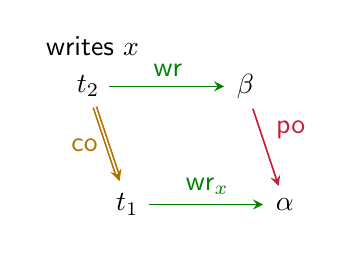
\begin{tikzpicture}[->,>=stealth,shorten >=1pt,auto,node distance=1cm,
					semithick, transform shape]
					\node[transaction state, text=black] at (0,0)       	(t_1)           {$t_1$};
					\node[transaction state, text=black, label={above:\textcolor{black}{$\writeVar{ }{x}$}}] at (-0.5,1.5) (t_2) {$t_2$};
					\node[transaction state, text=black] at (2,0)       (o_1)           {$\alpha$};
					\node[transaction state] at (1.5,1.5) (o_2) {$\beta$};
					\path (t_1) edge[color=wrColor] node {$\wro_x$} (o_1);
					% \path (t_2) edge[blue] node {$\CO$} (t_1);
					\path (t_2) edge[color=wrColor] node {$\wro$} (o_2);
					\path (o_2) edge[color=poColor] node {$\po$} (o_1);
					\path (t_2) edge[left,double,color=coColor] node {$\co$} (t_1);
				\end{tikzpicture}
				\parbox{\textwidth}{
					$\forall x,\ \forall t_1, t_2,\ \forall \alpha.\ t_1\neq t_2\ \land$
					
					\hspace{4mm}$\tup{t_1,\alpha}\in \wro_x \land \writeVar{t_2}{x}\ \land$ 
					
					\hspace{9mm}$\tup{t_2,\alpha}\in\wro\circ\po$
					
					\hspace{14mm}$\implies \tup{t_2,t_1}\in\co$
				}
				%\end{align*}
				
				\caption{$\mathsf{Read\ Committed}$}
				\label{lock_rc_def}
			\end{subfigure}
			
			&     
			
			
			\begin{subfigure}[t]{.35\textwidth}
				\centering
				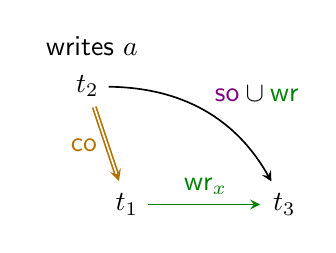
\begin{tikzpicture}[->,>=stealth,shorten >=1pt,auto,node distance=1cm,
					semithick, transform shape]
					\node[transaction state, text=black] at (0,0)       (t_1)           {$t_1$};
					\node[transaction state] at (2,0)       (t_3)           {$t_3$};
					\node[transaction state, text=black,label={above:\textcolor{black}{$\writeVar{ }{\xvar}$}}] at (-.5,1.5) (t_2) {$t_2$};
					\path (t_1) edge[wrColor] node {$\wro_x$} (t_3);
					% \path (t_2) edge[blue] node {$\CO$} (t_1);
					\path (t_2) edge[bend left] node {$\so \cup \wro$} (t_3);
					\path (t_2) edge[left, double ,coColor] node {$\co$} (t_1);
				\end{tikzpicture}
				\parbox{\textwidth}{
					$\forall x,\ \forall t_1, t_2,\ \forall t_3.\ t_1\neq t_2\ \land$
					
					\hspace{4mm}$\tup{t_1,t_3}\in \wro_x \land \writeVar{t_2}{x}\ \land$ 
					
					\hspace{9mm}$\tup{t_2,t_3}\in\so \cup \wro$
					
					\hspace{14mm}$\implies \tup{t_2,t_1}\in\co$
				}
				
				\caption{$\mathsf{Read\ Atomic}$}
				\label{ra_def}
			\end{subfigure}
			
			&
			
			\begin{subfigure}[t]{.31\textwidth}
				\centering
				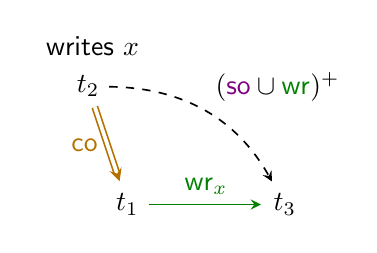
\begin{tikzpicture}[->,>=stealth,shorten >=1pt,auto,node distance=4cm,
					semithick, transform shape]
					\node[transaction state, text=black] at (0,0)       (t_1)           {$t_1$};
					\node[transaction state] at (2,0)       (t_3)           {$t_3$};
					\node[transaction state, text=black,label={above:\textcolor{black}{$\writeVar{ }{\key}$}}] at (-.5,1.5) (t_2) {$t_2$};
					\path (t_1) edge[wrColor] node {$\wro_x$} (t_3);
					% \path (t_2) edge[blue] node {$\CO$} (t_1);
					\path (t_2) edge[dashed, bend left] node {$(\so \cup \wro)^+$} (t_3);
					%   \path [->, decoration={snake}] (t_2) edge[decorate] node[auto] {F} (t_3);
					\path (t_2) edge[left,double equal sign distance,coColor] node {$\co$} (t_1);
				\end{tikzpicture}
				\parbox{\textwidth}{
					$\forall x,\ \forall t_1, t_2,\ \forall t_3.\ t_1\neq t_2\ \land$
					
					\hspace{4mm}$\tup{t_1,t_3}\in \wro_x \land \writeVar{t_2}{x}\ \land$ 
					
					\hspace{9mm}$\tup{t_2,t_3}\in(\so \cup \wro)^+$
					
					\hspace{14mm}$\implies \tup{t_2,t_1}\in\co$
				}
				
				\caption{$\mathsf{Causal\ Consistency}$}
				\label{cc_def}
			\end{subfigure}
			
			\\ \hline			  
			
			
			\begin{subfigure}[b]{.31\textwidth}
			\centering
			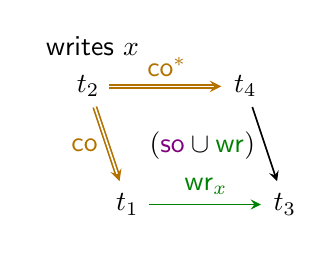
\begin{tikzpicture}[->,>=stealth,shorten >=1pt,auto,node distance=4cm,
			 semithick, transform shape]
			\node[transaction state, text=black] at (0,0)       (t_1)           {$t_1$};
			\node[transaction state] at (2,0)       (t_3)           {$t_3$};
			\node[transaction state, text=black,label={above:\textcolor{black}{$\writeVar{ }{x}$}}] at (-0.5,1.5) (t_2) {$t_2$};
			\node[transaction state] at (1.5,1.5) (t_4) {$t_4$};
			\path (t_1) edge[wrColor] node {$\wro_x$} (t_3);
			% \path (t_2) edge[blue] node {$\CO$} (t_1);
			\path (t_2) edge[coColor, double] node {$\co^*$} (t_4);
			\path (t_4) edge[left] node {$(\so \cup \wro)$} (t_3);
			\path (t_2) edge[left,double, coColor] node {$\co$} (t_1);
			\end{tikzpicture}
			\parbox{\textwidth}{
			$\forall \xvar,\ \forall t_1, t_2,\ \forall t_3.\ t_1\neq t_2\ \land$
			
			\hspace{4mm}$\tup{t_1,t_3}\in \wro_x \land \writeVar{t_2}{\xvar}\ \land$ 
			
			\hspace{9mm}$\tup{t_2,t_3}\in\co^*\circ\,(\wro\cup\so)$
			
			\hspace{14mm}$\implies \tup{t_2,t_1}\in\co$
			}
			
			\caption{$\mathsf{Prefix}$}
			\label{pre_def}
			\end{subfigure}
			     
			
			&
			\begin{subfigure}[b]{.35\textwidth}
			    \centering
			    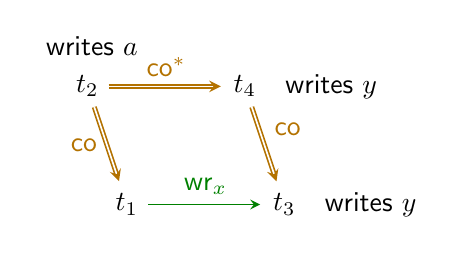
\begin{tikzpicture}[->,>=stealth,shorten >=1pt,auto,node distance=4cm,
			      semithick, transform shape]
			     \node[transaction state, text=black] at (0,0)       (t_1)           {$t_1$};
			     \node[transaction state, label={right:$\writeVar{ }{\yvar}$}] at (2,0)       (t_3)           {$t_3$};
			     \node[transaction state, text=black,label={above:\textcolor{black}{$\writeVar{ }{\xvar}$}}] at (-.5,1.5) (t_2) {$t_2$};
			     \node[transaction state, label={right:{$\writeVar{}{\yvar}$}}] at (1.5,1.5) (t_4) {$t_4$};
			     \path (t_1) edge[wrColor] node {$\wro_x$} (t_3);
			     % \path (t_2) edge[blue] node {$\CO$} (t_1);
			     \path (t_2) edge [coColor, double] node {$\co^*$} (t_4);
			     \path (t_4) edge [coColor, double] node {$\co$} (t_3);
			     \path (t_2) edge[left,double, coColor] node {$\co$} (t_1);
			    \end{tikzpicture}
			    \parbox{\textwidth}{
			     $\forall \xvar,\ \forall t_1, t_2,\ \forall t_3, t_4,\ \forall \yvar.\ t_1\neq t_2\ \land$
			     
			     \hspace{4mm}$\tup{t_1,t_3}\in \wro_x \land \writeVar{t_2}{\xvar}\ \land$ 
			     
			     \hspace{9mm}$\writeVar{t_3}{\yvar}\ \land \writeVar{t_4}{\yvar}\ \land$ 
			     
			     \hspace{12mm}$\tup{t_2,t_4}\in\co^*\ \land \tup{t_4,t_3}\in\co$
			     
			     \hspace{16mm}$\implies \tup{t_2,t_1}\in\co$
			    }
			    
			    \caption{$\mathsf{Conflict}$}
			    \label{confl_def}
			   \end{subfigure}
			&     
			\begin{subfigure}[b]{.31\textwidth}
				\centering
				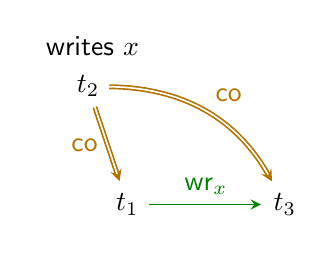
\begin{tikzpicture}[->,>=stealth,shorten >=1pt,auto,node distance=4cm,
					semithick, transform shape]
					\node[transaction state, text=black] at (0,0)       (t_1)           {$t_1$};
					\node[transaction state] at (2,0)       (t_3)           {$t_3$};
					\node[transaction state, text=black, label={above:\textcolor{black}{$\writeVar{ }{x}$}}] at (-.5,1.5) (t_2) {$t_2$};
					\path (t_1) edge[wrColor] node {$\wro_x$} (t_3);
					% \path (t_2) edge[blue] node {$\CO$} (t_1);
					\path (t_2) edge[bend left, double, coColor] node {$\co$} (t_3);
					\path (t_2) edge[left,double, coColor] node {$\co$} (t_1);
				\end{tikzpicture}
				\parbox{\textwidth}{
					$\forall x,\ \forall t_1, t_2,\ \forall t_3.\ t_1\neq t_2\ \land$
					
					\hspace{4mm}$\tup{t_1,t_3}\in \wro_x \land \writeVar{t_2}{x}\ \land$ 
					
					\hspace{9mm}$\tup{t_2,t_3}\in\co$
					
					\hspace{14mm}$\implies \tup{t_2,t_1}\in\co$
				}
				
				\caption{$\mathsf{Serializability}$}
				\label{ser_def}
			\end{subfigure}
		
		\\\hline
		\end{tabular}
	}
	%  \vspace{-3mm}
	\caption{Axioms defining isolations levels. The reflexive and transitive, resp., transitive, closure of a relation $rel$ is denoted by $rel^*$, resp., $rel^+$. Also, $\circ$ denotes the composition of two relations, i.e., $rel_1 \circ rel_2 = \{\tup{a, b} | \exists c. \tup{a, c} \in rel_1 \land \tup{c, b} \in rel_2\}$.}
	\label{fig:consistency_defs}
	%  \vspace{-2mm}
\end{figure}

A history is said to satisfy a certain isolation level if there exists a strict total order $\co$ on its transaction logs, called \emph{commit order}, which extends the write-read relation and the session order, and which satisfies certain properties. These properties, called \emph{axioms}, relate the commit order with the session-order and the write-read relation in the history. 
%The axioms define mandatory $\co$ predecessors $\tr_2$ of a transaction $\tr_1$ that is read in the history. 
They are defined as 
first-order formulas of the following form:
\begin{align}
  & \forall \key,\ \forall \tr_1\neq \tr_2,\ \forall \tau.\ \nonumber\\
  & \hspace{3mm}  \tup{\tr_1,\tau}\in \wro[\key] \land \writeVar{\tr_2}{\key} \land \phi(\tr_2,\tau) \implies \tup{\tr_2,\tr_1}\in\co \label{eq:axiom}
%  & \hspace{5.4cm} \implies \tup{\tr_2,\tr_1}\in\co \nonumber
\end{align}
where $\phi$ is a property relating $\tr_2$ and $\tau$ (i.e., the read or the
transaction reading from $\tr_1$) that varies from one axiom to another.\footnote{These formulas are interpreted on tuples $\tup{\hist,\co}$ of a history $\hist$ and a commit order $\co$ on the transactions in $\hist$ as usual.}  Intuitively, this axiom schema states the following: in order for $\tau$ to read specifically $t_1$'s write on $k$, it must be the case that every $t_2$ that also writes $k$ and satisfies $\phi(t_2,\tau)$ was committed before $t_1$. 
%Note that in all cases we consider, $\phi(t_2,\tau)$ already ensures that $t_2$ is committed before the read $\tau$, so this axiom schema ensures that $t_2$ is furthermore committed before $t_1$'s write.
The property $\phi$ relates $\tr_2$ and $\tau$ using the relations in a history and the commit order. 
Figure~\ref{fig:consistency_defs} shows four axioms which correspond to their homonymous isolation levels: \textit{Read Committed} ($\RC$), \textit{Read Atomic} ($\RA$), \textit{Causal Consistency} ($\CC$), and \textit{Serializability} ($\SER$). The conjunction of the other two axioms Conflict and Prefix defines \textit{Snapshot Isolation} ($\SI$). Note that $\SER$ is stronger than $\SI$ (i.e., every history satisfying $\SER$ satisfies $\SI$ as well), $\SI$ is stronger than $\CC$, $\CC$ is stronger than $\RA$, and $\RA$ is stronger than $\RC$.
% as the model where prefix and conflict axioms both hold. 
%We say a history $h$ satisfies an isolation level $I$ if there is a total order called \callout{commit order} $\co$ that extend $\so \cup \wro$ and satisfies its axioms. However, by the definition of $\RC, \RA$ and $\CC$, it is clear that for every history $h$ s.t. the relation $\co$ deduced from $\so \cup \wro$ is acyclic exists a commit order for those isolation levels.
%Figure~\ref{fig:consistency_defs} shows the axioms defining Read Committed, Causal Consistency, and Serializability (see \citet{DBLP:journals/pacmpl/BiswasE19} for axioms defining Read Atomic, Prefix, and Snapshot Isolation). 



%For instance, $\mathsf{Read\ Committed}$~\cite{DBLP:conf/sigmod/BerensonBGMOO95} requires that every read returns a value written in a committed transaction, and also, that the reads in the same transaction are ``monotonic'', i.e., they do not return values that are older, w.r.t. the commit order, than values read in the past.
%%\footnote{This monotonicity property corresponds to the fact that in the original formulation of $\mathsf{Read\ Committed}$~\cite{DBLP:conf/sigmod/BerensonBGMOO95}, every write is guarded by the acquisition of a lock on the written key, that is held until the end of the transaction.}. 
%While the first condition holds for every history (because of the surjectivity of $\wro$), the second condition is expressed by the axiom $\mathsf{Read\ Committed}$ in Figure~\ref{lock_rc_def}, which states that for any transaction $\tr_1$ writing a key $\key$ that is read at an operaion $\alpha$ in a transaction, the set of transactions $\tr_2$ writing $\key$ and read previously in the same transaction (these reads may concern other keys) must precede $\tr_1$ in commit order. 
%For instance, Figure~\ref{rc_example:1} shows a history and a (partial) commit order that does not satisfy this axiom because $\rd{\key_1}{1}$ returns the value written in a transaction ``older'' than the transaction read in the previous $\rd{\key_2}{2}$. %An exa


\begin{figure}
  
   \centering
%   \begin{subfigure}{.3\textwidth}
%  \resizebox{\textwidth}{!}{
%\begin{tikzpicture}[->,>=stealth',shorten >=1pt,auto,node distance=3cm,
%    semithick, transform shape]
%    \node[draw, rounded corners=2mm] (t1) at (0, 0) {\begin{tabular}{l} $\wrt{\key_1}{1}$ \end{tabular}};
%   \node[draw, rounded corners=2mm,outer sep=0] (t2) at (0, -1.5) {\begin{tabular}{l} $\wrt{\key_1}{2}$ \\ $\wrt{\key_2}{2}$\end{tabular}};
%   \node[draw, rounded corners=2mm, minimum width=1.8cm, minimum height=2.5cm] (t3) at (3, -0.75) {};
%   \node[style={inner sep=0,outer sep=0}] (t3_1) at (3, 0) {\begin{tabular}{l} $\rd{\key_2}{2}$ \end{tabular}};
%   \node[style={inner sep=0,outer sep=0}] (t3_2) at (3, -1.5) {\begin{tabular}{l} $\rd{\key_1}{1}$ \end{tabular}};
%   % \path (t1) edge node {} (t3_2);
%   % \path (t2) edge node {} (t3_1);
%   \path (t1) edge node {$\co$} (t2);
%   \path (t3_1) edge node {$\po$} (t3_2);
%   \path (t1) edge[below] node[yshift=-4,xshift=4] {$\wro$} (t3_2);
%   \path (t2) edge node[yshift=-2,xshift=7] {$\wro$} (t3_1);
%  \end{tikzpicture}  
%    }
%    \caption{$\mathsf{Read\ Committed}$ violation.}
%    \label{rc_example:1}
%\end{subfigure}
%\hspace{1cm}
\begin{subfigure}{.4\textwidth}
\resizebox{\textwidth}{!}{
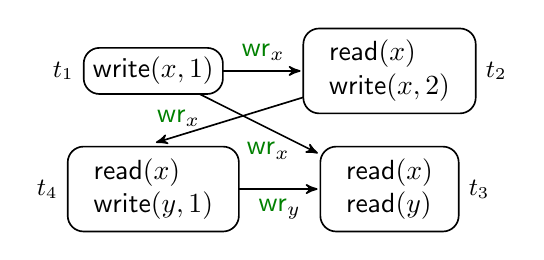
\begin{tikzpicture}[->,>=stealth',shorten >=1pt,auto,node distance=3cm,
 semithick, transform shape]
 \node[draw, rounded corners=2mm,outer sep=0, label={[font=\small]180:$t_1$}] (t1) at (0, 1.5) {$\ewrt{x,1}$};
\node[draw, rounded corners=2mm,outer sep=0,label={[font=\small]0:$t_2$}] (t2) at (3, 1.5) {\begin{tabular}{l} $\erd{x}$ \\ $\ewrt{x,2}$ \end{tabular}};
\node[draw, rounded corners=2mm,outer sep=0,label={[font=\small]0:$t_3$}] (t3) at (3, 0) {\begin{tabular}{l} $\erd{x}$ \\ $\erd{y}$ \end{tabular}};
\node[draw, rounded corners=2mm,outer sep=0,label={[font=\small]180:$t_4$}] (t4) at (0, 0) {\begin{tabular}{l} $\erd{x}$ \\ $\ewrt{y,1}$\end{tabular}};

\path (t1) edge[above] node[yshift=0,xshift=0] {$\wro_x$} (t2);

\path (t1) edge[below] node[yshift=-3,xshift=3] {$\wro_x$} (t3);

\path (t2) edge[above] node[yshift=-6,xshift=-18] {$\wro_x$} (0,0.58);

\path (t4) edge[below] node[yshift=0,xshift=0] {$\wro_y$} (t3);
\end{tikzpicture}  
}
% \caption{Causal C violation.}
% \label{cc_example:1}
\end{subfigure}
%\vspace{-3mm}
  \caption{Causal Consistency violation. Boxes group events from the same transaction.}
  \label{counter_example:1}
%\vspace{-3mm}
\end{figure}

For instance, the axiom defining Causal Consistency~\cite{DBLP:journals/cacm/Lamport78} states that for any transaction $\tr_1$ writing a variable $x$ that is read in a transaction $\tr_3$, the set of $(\wro\cup \so)^+$ predecessors of $\tr_3$ writing $x$ must precede $\tr_1$ in commit order ($(\wro\cup \so)^+$ is usually called the \emph{causal} order). A violation of this axiom can be found in Figure~\ref{counter_example:1}: the transaction $\tr_2$ writing 2 to $x$ is a $(\wro\cup \so)^+$ predecessor of the transaction $\tr_3$ reading 1 from $x$ because the transaction $\tr_4$, writing 1 to $y$, reads $x$ from $\tr_2$ and $\tr_3$ reads $y$ from $\tr_4$. This implies that $\tr_2$ should precede in commit order the transaction $\tr_1$ writing 1 to $x$, which again, is inconsistent with the write-read relation ($\tr_2$ reads from $\tr_1$).

The $\mathsf{Serializability}$ axiom requires that for any transaction $\tr_1$ writing to a variable $x$ that is read in a transaction $\tr_3$, the set of $\co$ predecessors of $\tr_3$ writing $x$ must precede $\tr_1$ in commit order. This ensures that each transaction observes the effects of all the $\co$ predecessors. 

%It was shown in~\cite{DBLP:journals/pacmpl/BiswasE19} that as expected, $\mathsf{Serializability}$ implies $\mathsf{Causal}$, which implies $\mathsf{Read\ Committed}$ (when interpreted as first-order formulas).

\begin{definition}
For an isolation level $I$ defined by a set of axioms $X$, a history
$\hist=\tup{T, \so, \wro}$ \emph{satisfies} $I$ iff there is a strict total
order $\co$ s.t. $\wro\cup\so\subseteq \co$ and $\tup{h,\co}$ satisfies $X$.\footnote{Isolation levels like Snapshot Isolation require more than one axiom.}
 % Given a $\CO$(\textit{commit order}), a total order on $T$ which extends $\wro \cup \so$, we can define consistency axioms from table \ref{consistency_defs}. For each axiom, the situation in the table implies, $\Path{\tr_2}{\CO}{\tr_1}$.
 \label{axiom-criterion}
\end{definition}

A history that satisfies an isolation level $I$ is called $I$-consistent.

%=====
%
%To fully model any behavior of a transactional concurrent program we are obliged to formally describe the database section. This notion will be depicted as the concept of \textit{model}:
%
%%Those notions are generic enough to only describe a possible set of instructions that a parallel program may execute along with the $\wr$ relations that exist between them.
%
%\begin{comment}
%\begin{definition}
%An axiomatic \callout{model} $\mathcal{M}$ over histories is a collection of rules that enforce a \callout{consistency criterion} over them. The histories that satisfy those criteria are called \callout{consistent} while the rest are simply denoted inconsistent. 
%\end{definition}
%\end{comment}
%
%\begin{definition}
%An axiomatic \callout{model} $\mathcal{M}$ over histories is a collection of rules that enforce a \callout{consistency criterion} over them. The histories that satisfy those criteria are called \callout{$\mathcal{M}$-consistent} while the rest are simply denoted $\mathcal{M}$-inconsistent. If there is no ambiguity on the model, we will simply denote them consistent or inconsistent.%
%
%\end{definition}
%
%
%
%In figure \ref{fig:consistency_defs} it is depicted five axioms which correspond to their homonymous isolation levels: \textit{Read Committed} ($\RC$), \textit{Read Atomic} ($\RA$), \textit{Causal Consistency} ($\CC$)  \textit{Prefix Consistency} ($\PRE$) and \textit{Serializability} ($\SER$); along with the conflict axiom. Conflict and Prefix allow us to define \textit{Snapshot Isolation} ($\SI$) as the model where prefix and conflict axioms both hold. We say a history $h$ satisfies an isolation level $I$ if there is a total order called \callout{commit order} $\co$ that extend $\so \cup \wro$ and satisfies its axioms. However, by the definition of $\RC, \RA$ and $\CC$, it is clear that for every history $h$ s.t. the relation $\co$ deduced from $\so \cup \wro$ is acyclic exists a commit order for those isolation levels.
%
%TODO DEFINE $I$-consistent histories

\subsection{Program Semantics}\label{ssec:semantics}

\begin{figure} [t]
\small
  \centering
  \begin{mathpar}
    \inferrule[spawn]{\tr \mbox{ fresh}\quad e \mbox{ fresh}\quad  \mathsf{P}(j) = \ibegin; \mathsf{Body}; \icommit; \mathsf{S} \quad \vec{\mathsf{B}}(j) = \epsilon}{
      \hist,\vec{\gamma},\vec{\mathsf{B}},\mathsf{P}
      \Rightarrow_I
      \hist \oplus_j \tup{\tr,\{\tup{e,\ebegin}\},\emptyset},\vec{\gamma}[j\mapsto \emptyset],\vec{\mathsf{B}}[j\mapsto \mathsf{Body}; \icommit],\mathsf{P}[j\mapsto \mathsf{S}]
    } 

    \inferrule[if-true]{\psi(\vec{x})[x\mapsto \vec{\gamma}(j)(x): x\in\vec{x}]\mbox{ true} \\
    \vec{\mathsf{B}}(j) = \iif{\psi(\vec{x})}{\mathsf{Instr}};\mathsf{B}
    }{
      \hist,\vec{\gamma},\vec{\mathsf{B}}, \mathsf{P}
      \Rightarrow_I
      \hist,\vec{\gamma},\vec{\mathsf{B}}[j\mapsto \mathsf{Instr};\mathsf{B}],\mathsf{P}
    } 

    \inferrule[if-false]{\psi(\vec{x})[x\mapsto \vec{\gamma}(j)(x): x\in\vec{x}]\mbox{ false} \\
    \vec{\mathsf{B}}(j) = \iif{\psi(\vec{x})}{\mathsf{Instr}};\mathsf{B}
    }{
      \hist,\vec{\gamma},\vec{\mathsf{B}}, \mathsf{P}
      \Rightarrow_I
      \hist,\vec{\gamma},\vec{\mathsf{B}}[j\mapsto \mathsf{B}],\mathsf{P}
    } 

    \inferrule[local]{v = \vec{\gamma}(j)(e) \\ \vec{\mathsf{B}}(j) = a := e;\mathsf{B}
    }{
      \hist,\vec{\gamma},\vec{\mathsf{B}}, \mathsf{P}
      \Rightarrow_I
      \hist,\vec{\gamma}[(j,\xvar)\mapsto \val],\vec{\mathsf{B}}[j\mapsto \mathsf{B}],\mathsf{P}
    } 

    \inferrule[write]{v = \vec{\gamma}(j)(x)\quad e\mbox{ fresh} \quad 
    \vec{\mathsf{B}}(j) = \iwrite(\key,\xvar);\mathsf{B}\quad \hist \oplus_j \tup{e,\ewrt{\key,\val}}\mbox{ satisfies $I$}
    }{
      \hist,\vec{\gamma},\vec{\mathsf{B}}, \mathsf{P}
      \Rightarrow_I
      \hist \oplus_j \tup{e,\ewrt{\key,\val}},\vec{\gamma},\vec{\mathsf{B}}[j\mapsto \mathsf{B}], \mathsf{P}
    } 

    \inferrule[read-local]{
    \writeOp{\mathit{last}(\hist,j)}\mbox{ contains a }\wrt{\key}{\val}\mbox{ event}\\
    e\mbox{ fresh } \\
    \vec{\mathsf{B}}(j) = \xvar := \iread(\key);\mathsf{B}
    }{
      \hist,\vec{\gamma},\vec{\mathsf{B}}, \mathsf{P}
      \Rightarrow_I
      \hist \oplus_j \tup{e,\erd{\key}},\vec{\gamma}[(j,\xvar)\mapsto \val],\vec{\mathsf{B}}[j\mapsto \mathsf{B}],\mathsf{P}
    } 

    \inferrule[read-extern]{
    \writeOp{\mathit{last}(\hist,j)}\mbox{ does not contain a }\wrt{\key}{\val}\mbox{ event} \\
    e\mbox{ fresh }\\
    \vec{\mathsf{B}}(j) = \xvar := \iread(\key);\mathsf{B} \\
    \hist=(T,\so,\wro) \\
    \tr =\mathit{last}(\hist,j) \\
    \wrt{\key}{\val}\in\writeOp{\tr'}\mbox{ with $\tr'\in \transC{\hist}$ and $\tr\neq \tr'$} \\
    \hist' = (\hist \oplus_j \tup{e,\erd{\key}}) \oplus \wro(\tr',e) \\
    \hist' \mbox{ satisfies }I }{
      \hist,\vec{\gamma},\vec{\mathsf{B}}, \mathsf{P}
      \Rightarrow_I
      \hist',\vec{\gamma}[(j,\xvar)\mapsto \val],\vec{\mathsf{B}}[j\mapsto \mathsf{B}],\mathsf{P}
    } 

    \inferrule[commit]{e\mbox{ fresh} \quad 
    \vec{\mathsf{B}}(j) = \icommit 
    }{
      \hist,\vec{\gamma},\vec{\mathsf{B}}, \mathsf{P}
      \Rightarrow_I
      \hist \oplus_j \tup{e,\icommit},\vec{\gamma},\vec{\mathsf{B}}[j\mapsto \epsilon], \mathsf{P}
    } 
  \end{mathpar}
% \vspace{-5mm}
  \caption{An operational semantics for transactional programs. Above, $\mathit{last}(h,j)$ denotes the last transaction log in the session order $\so(j)$ of $h$, and $\transC{\hist}$ denotes the set of transaction logs in $\hist$ that are complete.}
  \label{fig:op:sem:baseline}
\end{figure}

We define a small-step operational semantics for transactional programs, which is parametrized by an isolation level $I$. The semantics keeps a history of previously executed database accesses in order to maintain consistency with $I$. 

For readability, we define a program as a partial function $\prog:\mathsf{SessId}\rightharpoonup \mathsf{Sess}$ that associates session identifiers in $\mathsf{SessId}$ with concrete code as defined in Figure~\ref{fig:syntax} (i.e., sequences of transactions). Similarly, the session order $\so$ in a history is defined as a partial function $\so:\mathsf{SessId}\rightharpoonup \mathsf{Tlogs}^*$ that associates session identifiers with sequences of transaction logs. Two transaction logs are ordered by $\so$ if one occurs before the other in some sequence $\so(j)$ with 
$j\in \mathsf{SessId}$.

Formally, the operational semantics is defined as a transition relation $\Rightarrow_I$ between \emph{configurations}, which are defined as tuples containing the following:
\begin{itemize}
	\item history $\hist$ storing the events generated by database accesses executed in the past, 
	\item a valuation map $\vec{\gamma}$ that records local variable values in the current transaction of each session ($\vec{\gamma}$ associates identifiers of sessions that have live transactions with valuations of local variables),
	\item a map $\vec{B}$ that stores the code of each live transaction (associating session identifiers with code), and
	\item sessions/transactions $\prog$ that remain to be executed from the original program.
\end{itemize}



Before presenting the definition of $\Rightarrow_I$, we introduce some notation. Let $\hist$ be a history that contains a representation of $\so$ as above. We use $\hist\oplus_j \tup{\tr,E,\po_t}$ to denote a history where $\tup{\tr,E,\po_t}$ is appended to $\so(j)$. 
Also, for an event $e$, $\hist\oplus_j e$ is the history obtained from $\hist$ by adding $e$ to the last transaction log in $\so(j)$ and as a last event in the program order of this log (i.e.,  if $\so(j)=\sigma; \tup{t,E,\po_t}$, then the session order $\so'$ of $\hist\oplus_j e$ is defined by $\so'(k)=\so(k)$ for all $k\neq j$ and $\so(j) =\sigma; \tup{t,E\cup\{e\},\po_t\cup \{(e',e): e'\in E\}}$). Finally, for a history $\hist = \tup{T, \so, \wro}$, $\hist\oplus\wro(\tr,e)$ is the history obtained from $\hist$ by adding $(\tr,e)$ to the write-read relation.

Figure~\ref{fig:op:sem:baseline} lists the rules defining $\Rightarrow_I$. %(the others can be defined in a similar manner). 
\textsc{spawn} starts a new transaction in a session $j$ provided that this session has no live transaction ($\vec{\mathsf{B}}(j) = \epsilon$). It adds a transaction log with a single $\ebegin$ event to the history and schedules the body of the transaction. \textsc{if-true} and \textsc{if-false} check the truth value of a Boolean condition of an $\mathtt{if}$ conditional. \textsc{local} models the execution of an assignment to a local variable which does not impact the stored history. \textsc{read-local} and \textsc{read-extern} concern read instructions. \textsc{read-local} handles the case where the read follows a write on the variable $x$ in the same transaction: the read returns the value written by the last write on $x$ in that transaction. Otherwise, \textsc{read-extern} corresponds to reading a value written in another transaction $\tr'$. The transaction $\tr'$ is chosen non-deterministically as long as extending the current history with the write-read dependency associated to this choice leads to a history that still satisfies $I$. \textsc{read-extern} applies only when the executing transaction contains no write on the same variable.

An \emph{initial} configuration for program $\prog$ contains the program $\prog$ along with a history $\hist=\tup{\{\tr_0\},\emptyset,\emptyset}$, where $\tr_0$ is a transaction log containing only writes that write the initial values of all variables, and empty current transaction code ($\mathsf{B}=\epsilon$). 
An execution of a program $\prog$ under an isolation level $I$ is a sequence of configurations $c_0 c_1\ldots c_n$ where $c_0$ is an initial configuration for $\prog$, and $c_m\Rightarrow_I c_{m+1}$, for every $0\leq m < n$. We say that $c_n$ is \emph{$I$-reachable} from $c_0$.
The history of such an execution is the history $\hist$ in the last configuration $c_n$. 
A configuration is called \emph{final} if it contains the empty program ($\prog=\emptyset$).
Let $\histOf[I]{\prog}$ denote the set of all histories of an execution of $\prog$ under $I$ that ends in a final configuration.


%	\section{Definitions}

In this section we describe the basic concepts STMC is built on along with the assumptions required for its correctness.

%During the whole paper, we will work between different finite well-ordered domains: $\mathcal{I}$, $\mathcal{P}$,$\mathcal{P}$, $\mathcal{X}$, $\mathcal{V}$, $\mathcal{E}$ and $\mathcal{T}$ which represent 
\begin{definition}
An \callout{event} $e$ is a tuple $\langle id, t \rangle$ where $id$ is its \callout{identifier} and $t$ its \callout{type}. The set of all events will be denoted $\mathcal{E}$.
\end{definition}

Intuitively, an event $e$ represents an instruction on the program and its identifier is the line number this instruction has on it. However, this description forces us to have a wide range of possible types; one per instruction types. As we want to model check transactional programs, only those instructions related with our database are actually meaningful. Therefore, an event $e$ would represent a succession of local instructions followed by a database instruction; instruction of type $\ibegin, \iend, \iwrite$ or $\iread$. 

Further, we define a function called \callout{variable}, $\texttt{var}: \mathcal{E} \to \mathcal{V}$, which if $e$'s type is $\iwrite$ or $\iread$ returns the variable it writes/reads in the database and another function called \callout{value}, $\texttt{val}: \mathcal{E} \to \mathbb{N}$, that for every $\iwrite$ $w$ event returns the value that $\variable{w}$ will store after its execution. Note that for simplicity we assume $\valEvent{\mathcal{E}} \subseteq \mathbb{N}$, but the actual value of the instruction could be any computable binary string; string representable in $\mathbb{N}$. Nonetheless, for clarity during our examples we may write `` $a \gets \rd{x}$'' or ``$\wrt{x}{0}$'' as a succinct notation for indicate an event's type, its variable or its value.


%Every event can be unequivocally identified thanks to $id$ and $t$ is one of the following values $\{\ibegin, \iend, \iwrite, \iread\}$. Moreover, only $\iread$ and $\iwrite$ events involve variables, and only the latter has a value; so in every other case, its variable and/or value would be $\bot$.%Moreover, if $t$ is $\ibegin$ or $\iend$, $x$ and $v$ have the special value $\bot$; while if $t = \iread$, only $v$ ha $\bot$. If $e.type() = \iread$ and $e.value() = \bot$ we say that $e$ is \callout{free}; otherwise the event is \callout{fixed}. 

\begin{definition}
A \callout{transaction} $T$ is a finite sequence of events totally ordered by $\po_T$ where $\min_{\po_T}T$ has type $\ibegin$, $\max_{\po_T}T$ has type $\iend$ and every other event in $T$ is either a $\iread$ or $\iwrite$ event. Any $\po$-closed prefix of a transaction is called \callout{pending transaction}.
\end{definition}

%For every transaction $T$, we denote $\po_T$ the total order existing between the events in $T$.
During the whole paper we will assume that every pair of transactions are disjoint and that both $\mathcal{E}$ and $\mathcal{T}$ are finite. Therefore, we denote the function $tr: \mathcal{E} \to \mathcal{T}$ that associates every event to the unique transaction it belongs to. %Moreover, we will assume there is a special transaction called \callout{initial} that contains exactly one write event for every possible variable.

\begin{definition}
A \callout{program} $\mathcal{P}_{n, \mathcal{T}}$ is the collection of $n$ parallel threads that execute each a sequence of transactions. %execute in isolation every transaction in $\mathcal{T}$. Two different threads don't share any event in common, every thread enforce a total order between its transactions and the program's execution is always preceded by an \callout{initial transaction} (which gives an initial value to every variable). %Every thread execute its own set of transactions, producing a strict partial order $\so$ in $\mathcal{T}$ called \callout{session order}.
\end{definition}

In what follows, we will assume a fixed program $\mathcal{P}$ in order to slightly relax the notation. We also assume that every transaction is included in exactly one thread, so we can map every event to the thread it belongs to via the function $\texttt{th}_{\mathcal{P}} : \mathcal{E} \to \mathbb{Z}_n$.

For representing executions in a program we rely on the definition \ref{def:histories}, which allow us representing executions as execution graphs \textcolor{red}{cite paper} where the vertices are transactions and the edges are their relations.

\begin{definition}
\label{def:histories}
A \callout{history} $h = \langle T, \so, \wro \rangle$ is a tuple composed by a set of (pending) transactions $T$ (constructed over an event set $E \subseteq \mathcal{E}$) along with a strict partial order $\so$ called \callout{session order} and a relation $\wro \subseteq \writeOp{E} \times \readOp{E}$ called \callout{write-read} s.t.
\begin{itemize}
\item $\wro^{-1}$ is a total function,
\item $\so$ corresponds to the strict partial order defined by every thread in $\mathcal{P}$ restricted to $T$,
\item $\so \cup \wro$ is acyclic.
\end{itemize}

\end{definition}

We denote by $\emptyset$ the history with no vertices and we also write, with an abuse of notation, $T \ [\wro] \  T'$ whenever $\exists w, r \in T \times T'$ such that $w \ [\wro] \ r $. Finally, we briefly define several type of histories in next definition:

%From this point onward, we will assume that histories are $(\so \cup \bigcup\limits_{T \in \mathcal{T}}{\po_T})$-maximal, i.e. for every pair of events $e,e'$, if $e \ [\po_T] \ e'$ for some $T$ or $e \ [\so] \ e'$ and $e' \in h$, then $e \in h$. Moreover, we will also assume that every event in $h$ is fixed and for every pair of events $w,r$ $\wro$-related such that $r \in h$, $w$ is also in $h$. Those histories will be called \callout{coherent}. We will also denote by $\emptyset$ to the empty history, i.e. the one with no vertices. 

%The order enforced to the $T$ (and therefore, to $E$) is called \callout{history order} and denoted as $<_h$.

%In addition, we also write with an abuse of notation $T \ [\wro] \  T'$ whenever $\exists w, r \in T \times T'$ such that $w \ [\wro] \ r $. 

\begin{definition}
Let $h$ be a history:
\begin{itemize}
\item $h$ is called \callout{complete} if every transaction is non-pending and \callout{incomplete} otherwise;
\item $h$ is \callout{executed in isolation} if it contains at most one pending transaction;
\item $h$ is called \callout{total} if it is complete and contains every transaction $T \in \mathcal{T}$.
\end{itemize}
\end{definition}

\textcolor{red}{EXTENSIONS AND $\bullet$ OPERATOR NOT (yet) DEFINED IN THIS SECTION!!!!!!!}

To fully model any behavior of a transactional concurrent program we are obliged to formally describe the database section. This notion will be depicted as the concept of \textit{model}:

%Those notions are generic enough to only describe a possible set of instructions that a parallel program may execute along with the $\wr$ relations that exist between them.

\begin{comment}
\begin{definition}
An axiomatic \callout{model} $\mathcal{M}$ over histories is a collection of rules that enforce a \callout{consistency criterion} over them. The histories that satisfy those criteria are called \callout{consistent} while the rest are simply denoted inconsistent. 
\end{definition}
\end{comment}

\begin{definition}
An axiomatic \callout{model} $\mathcal{M}$ over histories is a collection of rules that enforce a \callout{consistency criterion} over them. The histories that satisfy those criteria are called \callout{$\mathcal{M}$-consistent} while the rest are simply denoted $\mathcal{M}$-inconsistent. If there is no ambiguity on the model, we will simply denote them consistent or inconsistent.%

\end{definition}

\begin{figure}[H]
	\resizebox{\textwidth}{!}{
		\footnotesize
		\begin{tabular}{|c|c|c|}
			\hline &  & \\
			\begin{subfigure}[t]{.31\textwidth}
				\centering
				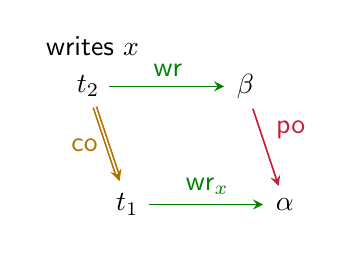
\begin{tikzpicture}[->,>=stealth,shorten >=1pt,auto,node distance=1cm,
					semithick, transform shape]
					\node[transaction state, text=black] at (0,0)       	(t_1)           {$t_1$};
					\node[transaction state, text=black, label={above:\textcolor{black}{$\writeVar{ }{x}$}}] at (-0.5,1.5) (t_2) {$t_2$};
					\node[transaction state, text=black] at (2,0)       (o_1)           {$\alpha$};
					\node[transaction state] at (1.5,1.5) (o_2) {$\beta$};
					\path (t_1) edge[color=wrColor] node {$\wro_x$} (o_1);
					% \path (t_2) edge[blue] node {$\CO$} (t_1);
					\path (t_2) edge[color=wrColor] node {$\wro$} (o_2);
					\path (o_2) edge[color=poColor] node {$\po$} (o_1);
					\path (t_2) edge[left,double,color=coColor] node {$\co$} (t_1);
				\end{tikzpicture}
				\parbox{\textwidth}{
					$\forall x,\ \forall t_1, t_2,\ \forall \alpha.\ t_1\neq t_2\ \land$
					
					\hspace{4mm}$\tup{t_1,\alpha}\in \wro_x \land \writeVar{t_2}{x}\ \land$ 
					
					\hspace{9mm}$\tup{t_2,\alpha}\in\wro\circ\po$
					
					\hspace{14mm}$\implies \tup{t_2,t_1}\in\co$
				}
				%\end{align*}
				
				\caption{$\mathsf{Read\ Committed}$}
				\label{lock_rc_def}
			\end{subfigure}
			
			&     
			
			
			\begin{subfigure}[t]{.35\textwidth}
				\centering
				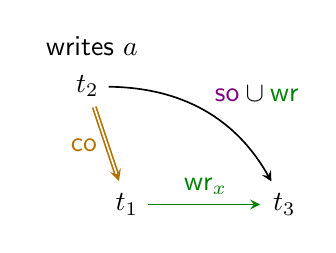
\begin{tikzpicture}[->,>=stealth,shorten >=1pt,auto,node distance=1cm,
					semithick, transform shape]
					\node[transaction state, text=black] at (0,0)       (t_1)           {$t_1$};
					\node[transaction state] at (2,0)       (t_3)           {$t_3$};
					\node[transaction state, text=black,label={above:\textcolor{black}{$\writeVar{ }{\xvar}$}}] at (-.5,1.5) (t_2) {$t_2$};
					\path (t_1) edge[wrColor] node {$\wro_x$} (t_3);
					% \path (t_2) edge[blue] node {$\CO$} (t_1);
					\path (t_2) edge[bend left] node {$\so \cup \wro$} (t_3);
					\path (t_2) edge[left, double ,coColor] node {$\co$} (t_1);
				\end{tikzpicture}
				\parbox{\textwidth}{
					$\forall x,\ \forall t_1, t_2,\ \forall t_3.\ t_1\neq t_2\ \land$
					
					\hspace{4mm}$\tup{t_1,t_3}\in \wro_x \land \writeVar{t_2}{x}\ \land$ 
					
					\hspace{9mm}$\tup{t_2,t_3}\in\so \cup \wro$
					
					\hspace{14mm}$\implies \tup{t_2,t_1}\in\co$
				}
				
				\caption{$\mathsf{Read\ Atomic}$}
				\label{ra_def}
			\end{subfigure}
			
			&
			
			\begin{subfigure}[t]{.31\textwidth}
				\centering
				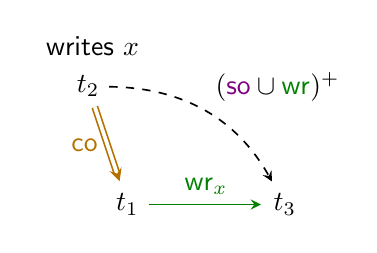
\begin{tikzpicture}[->,>=stealth,shorten >=1pt,auto,node distance=4cm,
					semithick, transform shape]
					\node[transaction state, text=black] at (0,0)       (t_1)           {$t_1$};
					\node[transaction state] at (2,0)       (t_3)           {$t_3$};
					\node[transaction state, text=black,label={above:\textcolor{black}{$\writeVar{ }{\key}$}}] at (-.5,1.5) (t_2) {$t_2$};
					\path (t_1) edge[wrColor] node {$\wro_x$} (t_3);
					% \path (t_2) edge[blue] node {$\CO$} (t_1);
					\path (t_2) edge[dashed, bend left] node {$(\so \cup \wro)^+$} (t_3);
					%   \path [->, decoration={snake}] (t_2) edge[decorate] node[auto] {F} (t_3);
					\path (t_2) edge[left,double equal sign distance,coColor] node {$\co$} (t_1);
				\end{tikzpicture}
				\parbox{\textwidth}{
					$\forall x,\ \forall t_1, t_2,\ \forall t_3.\ t_1\neq t_2\ \land$
					
					\hspace{4mm}$\tup{t_1,t_3}\in \wro_x \land \writeVar{t_2}{x}\ \land$ 
					
					\hspace{9mm}$\tup{t_2,t_3}\in(\so \cup \wro)^+$
					
					\hspace{14mm}$\implies \tup{t_2,t_1}\in\co$
				}
				
				\caption{$\mathsf{Causal\ Consistency}$}
				\label{cc_def}
			\end{subfigure}
			
			\\ \hline			  
			
			
			\begin{subfigure}[b]{.31\textwidth}
			\centering
			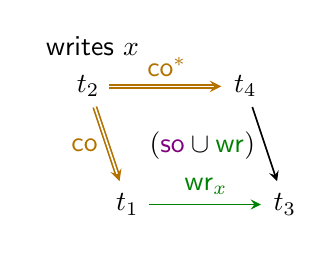
\begin{tikzpicture}[->,>=stealth,shorten >=1pt,auto,node distance=4cm,
			 semithick, transform shape]
			\node[transaction state, text=black] at (0,0)       (t_1)           {$t_1$};
			\node[transaction state] at (2,0)       (t_3)           {$t_3$};
			\node[transaction state, text=black,label={above:\textcolor{black}{$\writeVar{ }{x}$}}] at (-0.5,1.5) (t_2) {$t_2$};
			\node[transaction state] at (1.5,1.5) (t_4) {$t_4$};
			\path (t_1) edge[wrColor] node {$\wro_x$} (t_3);
			% \path (t_2) edge[blue] node {$\CO$} (t_1);
			\path (t_2) edge[coColor, double] node {$\co^*$} (t_4);
			\path (t_4) edge[left] node {$(\so \cup \wro)$} (t_3);
			\path (t_2) edge[left,double, coColor] node {$\co$} (t_1);
			\end{tikzpicture}
			\parbox{\textwidth}{
			$\forall \xvar,\ \forall t_1, t_2,\ \forall t_3.\ t_1\neq t_2\ \land$
			
			\hspace{4mm}$\tup{t_1,t_3}\in \wro[\xvar] \land \writeVar{t_2}{\xvar}\ \land$ 
			
			\hspace{9mm}$\tup{t_2,t_3}\in\co^*\circ\,(\wro\cup\so)$
			
			\hspace{14mm}$\implies \tup{t_2,t_1}\in\co$
			}
			
			\caption{$\mathsf{Prefix}$}
			\label{pre_def}
			\end{subfigure}
			     
			
			&
			\begin{subfigure}[b]{.35\textwidth}
			    \centering
			    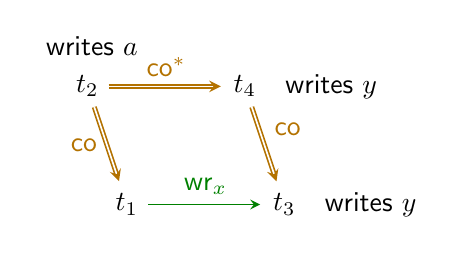
\begin{tikzpicture}[->,>=stealth,shorten >=1pt,auto,node distance=4cm,
			      semithick, transform shape]
			     \node[transaction state, text=black] at (0,0)       (t_1)           {$t_1$};
			     \node[transaction state, label={right:$\writeVar{ }{\yvar}$}] at (2,0)       (t_3)           {$t_3$};
			     \node[transaction state, text=black,label={above:\textcolor{black}{$\writeVar{ }{\xvar}$}}] at (-.5,1.5) (t_2) {$t_2$};
			     \node[transaction state, label={right:{$\writeVar{}{\yvar}$}}] at (1.5,1.5) (t_4) {$t_4$};
			     \path (t_1) edge[wrColor] node {$\wro_x$} (t_3);
			     % \path (t_2) edge[blue] node {$\CO$} (t_1);
			     \path (t_2) edge [coColor, double] node {$\co^*$} (t_4);
			     \path (t_4) edge [coColor, double] node {$\co$} (t_3);
			     \path (t_2) edge[left,double, coColor] node {$\co$} (t_1);
			    \end{tikzpicture}
			    \parbox{\textwidth}{
			     $\forall \xvar,\ \forall t_1, t_2,\ \forall t_3, t_4,\ \forall \yvar.\ t_1\neq t_2\ \land$
			     
			     \hspace{4mm}$\tup{t_1,t_3}\in \wro_x \land \writeVar{t_2}{\xvar}\ \land$ 
			     
			     \hspace{9mm}$\writeVar{t_3}{\yvar}\ \land \writeVar{t_4}{\yvar}\ \land$ 
			     
			     \hspace{12mm}$\tup{t_2,t_4}\in\co^*\ \land \tup{t_4,t_3}\in\co$
			     
			     \hspace{16mm}$\implies \tup{t_2,t_1}\in\co$
			    }
			    
			    \caption{$\mathsf{Conflict}$}
			    \label{confl_def}
			   \end{subfigure}
			&     
			\begin{subfigure}[b]{.31\textwidth}
				\centering
				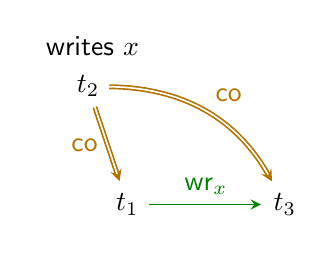
\begin{tikzpicture}[->,>=stealth,shorten >=1pt,auto,node distance=4cm,
					semithick, transform shape]
					\node[transaction state, text=black] at (0,0)       (t_1)           {$t_1$};
					\node[transaction state] at (2,0)       (t_3)           {$t_3$};
					\node[transaction state, text=black, label={above:\textcolor{black}{$\writeVar{ }{x}$}}] at (-.5,1.5) (t_2) {$t_2$};
					\path (t_1) edge[wrColor] node {$\wro_x$} (t_3);
					% \path (t_2) edge[blue] node {$\CO$} (t_1);
					\path (t_2) edge[bend left, double, coColor] node {$\co$} (t_3);
					\path (t_2) edge[left,double, coColor] node {$\co$} (t_1);
				\end{tikzpicture}
				\parbox{\textwidth}{
					$\forall x,\ \forall t_1, t_2,\ \forall t_3.\ t_1\neq t_2\ \land$
					
					\hspace{4mm}$\tup{t_1,t_3}\in \wro_x \land \writeVar{t_2}{x}\ \land$ 
					
					\hspace{9mm}$\tup{t_2,t_3}\in\co$
					
					\hspace{14mm}$\implies \tup{t_2,t_1}\in\co$
				}
				
				\caption{$\mathsf{Serializability}$}
				\label{ser_def}
			\end{subfigure}
		
		\\\hline
		\end{tabular}
	}
	%  \vspace{-3mm}
	\caption{Axioms defining isolations levels. The reflexive and transitive, resp., transitive, closure of a relation $rel$ is denoted by $rel^*$, resp., $rel^+$. Also, $\circ$ denotes the composition of two relations, i.e., $rel_1 \circ rel_2 = \{\tup{a, b} | \exists c. \tup{a, c} \in rel_1 \land \tup{c, b} \in rel_2\}$.}
	\label{fig:consistency_defs}
	%  \vspace{-2mm}
\end{figure}

In figure \ref{fig:consistency_defs} it is depicted five axioms which correspond to their homonymous isolation levels: \textit{Read Committed} ($\RC$), \textit{Read Atomic} ($\RA$), \textit{Causal Consistency} ($\CC$)  \textit{Prefix Consistency} ($\PRE$) and \textit{Serializability} ($\SER$); along with the conflict axiom. Conflict and Prefix allow us to define \textit{Snapshot Isolation} ($\SI$) as the model where prefix and conflict axioms both hold. We say a history $h$ satisfies an isolation level $I$ if there is a total order called \callout{commit order} $\co$ that extend $\so \cup \wro$ and satisfies its axioms. However, by the definition of $\RC, \RA$ and $\CC$, it is clear that for every history $h$ s.t. the relation $\co$ deduced from $\so \cup \wro$ is acyclic exists a commit order for those isolation levels.

%Because this is equivalent to state $\so \cup \wro \cup \co$ is an acylic relationm

%, they enforce some relation between transactions, represented as $\co$-edges. Under this three models we say a history is consistent if exists a total order called \callout{commit order}, $\co$, that extend $\so \cup \wro$ and satisfies the axioms. 
	\section{Maximal closed models}

\textcolor{red}{EXTENSIONS AND $\bullet$ OPERATOR NOT DEFINED IN THIS SECTION!!!!!!!}

Besides models presented in figure \ref{fig:consistency_defs}, others isolation levels exists in literature and real life applications \textcolor{red}{cite Constantin's papers + Twitter, shoppingcart...}. However, our algorithm can not be analyzed under an arbitrary model. We characterize in this section the ones that can be employed by our algorithm.
%not all of them can verified with the algorithm

\begin{figure}[H]
	
	\centering
	\begin{subfigure}[b]{.25\textwidth}
		\resizebox{\textwidth}{!}{
			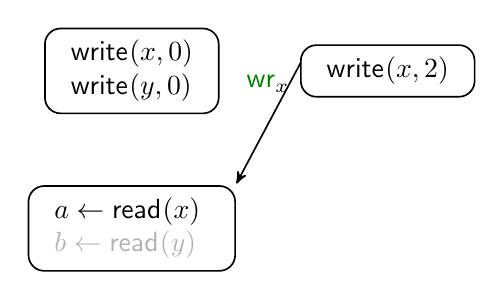
\begin{tikzpicture}[->,>=stealth',shorten >=1pt,auto,node distance=3cm,
				semithick, transform shape]
				\node[draw, rounded corners=2mm,outer sep=0] (t1) at (-3.25, 0) {\begin{tabular}{l} $\wrt{x}{0}$ \\ $\wrt{y}{0}$ \end{tabular}};
				\node[draw, rounded corners=2mm,outer sep=0] (t2) at (-3.25, -2) {\begin{tabular}{l} 
						$a \gets \rd{x}$ \pgfsetfillopacity{0.3}\\ $b \gets \rd{y}$
				\end{tabular}};
				\node[draw, rounded corners=2mm,outer sep=0] (t3) at (0, 0) {\begin{tabular}{l} 
						$\wrt{x}{2}$%\\
						%\pgfsetfillopacity{0.3}$\wrt{y}{2}$
				\end{tabular}};			
				
				\path (t1.south west) -- (t1.south) coordinate[pos=0.67] (t1x);
				\path (t2.north west) -- (t2.north) coordinate[pos=0.67] (t2x);
				\path (t3.north west) -- (t3.west) coordinate[pos=0.67] (t3x);
				
				\path (t3x) edge [above] node[yshift=8,xshift=0] {$\wro_x$} (t2.north east);
				%\path (t1x) edge [right] node {$\wro_y$} (t2x);
			\end{tikzpicture}  
			
		}
		\caption{Extensible history.}
		\label{fig:maxclosed:a}
	\end{subfigure}
	\hspace{.75cm}
	\centering
	\begin{subfigure}[b]{.25\textwidth}
		\resizebox{\textwidth}{!}{
			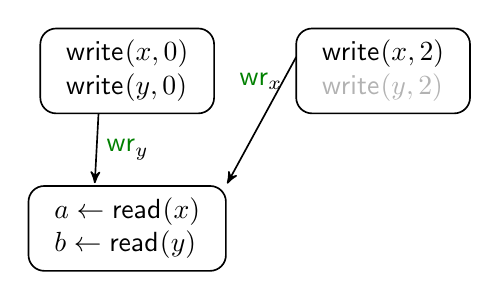
\begin{tikzpicture}[->,>=stealth',shorten >=1pt,auto,node distance=3cm,
				semithick, transform shape]
				\node[draw, rounded corners=2mm,outer sep=0] (t1) at (-3.25, 0) {\begin{tabular}{l} $\wrt{x}{0}$ \\ $\wrt{y}{0}$ \end{tabular}};
				\node[draw, rounded corners=2mm,outer sep=0] (t2) at (-3.25, -2) {\begin{tabular}{l} 
						$a \gets \rd{x}$ \\ $b \gets \rd{y}$
				\end{tabular}};
				\node[draw, rounded corners=2mm,outer sep=0] (t3) at (0, 0) {\begin{tabular}{l} 
						$\wrt{x}{2}$\pgfsetfillopacity{0.3}\\
						$\wrt{y}{2}$
				\end{tabular}};			
				
				\path (t1.south west) -- (t1.south) coordinate[pos=0.67] (t1x);
				\path (t2.north west) -- (t2.north) coordinate[pos=0.67] (t2x);
				\path (t3.north west) -- (t3.west) coordinate[pos=0.67] (t3x);
				
				\path (t3x) edge [above] node[yshift=8,xshift=0] {$\wro_x$} (t2.north east);
				\path (t1x) edge [right] node {$\wro_y$} (t2x);
			\end{tikzpicture}
			
		}
		\caption{Non-extensible history.}
		\label{fig:maxclosed:b}
	\end{subfigure}
	\hspace{.175cm}
	\centering
	\caption{Example of a dead-lock after swapping two events.}
	\label{fig:maxclosed}
	%\vspace{-3mm}
\end{figure}

Let's analyze the histories $h_1$ and $h_2$ described in figure \ref{fig:maxclosed:a} and \ref{fig:maxclosed:b} respectively under RA; isolation level under which both are consistent. $h_1$ can be extended adding the event $r_1 = b \gets \rd{y}$ and the $\wro$-edge $w_1 \ [\wro] \ r_1$, where $w_1 = \wrt{x}{0}$. However, this is not the case of $h_2$: the only event that could be added in it is $w_2 = \wrt{y}{2}$. If $w_2$ would be added in $h_2$, any relation extending $\so \cup \wro$ and satisfying RA would be cyclic, so it wouldn't be a commit order. The essential difference between these two histories is the following: in $h_1$, $\tr(r)$ is $\so \cup \wro$-maximal while in $h_2$ $\tr(w)$ is not. As real database executions forbid transactions reading from non-committed ones, it is reasonable to allow those transactions $\so \cup \wro$-maximal to be executed completed without hindering the previous committed transactions. 

\begin{definition}
A model $\mathcal{M}$ is called \callout{maximal closed} if for every program $\mathcal{P}$ the following conditions are satisfied:
\begin{itemize}
	%\item \textbf{Well-formedness:} Consistency criteria for a history $h$ only depend on the edges of $h$ and if $h$ is consistent then $[\so \cup \wro]^+$ is also acyclic.
	
	\item \textbf{Prefix-closedness:} Every $\so \cup \wro$-prefix-closed sub-history of a consistent history is also consistent.
	\item \textbf{Maximal-extensibility:} Every non-total consistent history $h$ can be consistently extended by executing an event from a $\so \cup \wro$-maximal pending transaction $T$ in $h$.
	\textcolor{orange}{\item \textbf{Past-readability:} For every history $h$ and every $\so \cup \wro$-maximal $\iread$ event $r$ there exists a $\iwrite$ event $w$ s.t. $h \bullet_w r$ is consistent and $r$ is not-swapped} \textcolor{red}{\textbf{NEW CONSTRAINT ADDED!!} \textbf{\underline{Swapped} not defined until a bit later!!} It is added as a constraint because it is stronger than maximal extensibility and only added in some small part of the proof (prev's correctness lemma). Nevertheless, it is an strengthening of maximal-extensibility; maybe it has to be adapted. } 
	

	  %Every non-total consistent history $h$ executed in isolation there is a complete consistent history $h'$ such that $h$ is a strict $\so \cup \wro$-prefix-closed sub-history of $h'$. In particular, adding a $\ibegin, \iwrite$ or $\iend$ to a history does not change its evaluation.
\end{itemize}
\end{definition}
%For be denominated as \callout{STMC-model}, $\mathcal{M}$ has to satisfies the following three axioms for every program $\mathcal{P}$:

Comparing to the model requirements described in \textcolor{red}{cite viktor's algorithm}, it is maximal-extensibility property the most weakened one. However, this weak formulation still forbids some axiomatic models such as Serializability \textcolor{red}{cite constantin's paper (SER)} to not be a maximal closed model \textcolor{red}{Appendix cite}.
%Indeed, some isolation levels cannot guarantee that reading from the last added $\iwrite$ event will maintain its consistency status.

\begin{theorem}
\label{theorem:maximalClosedModels}
Causal Consistency (CC), Read Atomic (RA) and Read Committed (RC) are maximal closed models.
\begin{proof}
$ $	
	
\underline{Prefix-closedness:} Let $h$ be a consistent history. As any $\so \cup \wro$-prefix-closed sub-history $h'$ of $h$ is a sub-graph of it, and there is a commit order $\co$ for $h$, it suffices to restrict $\co$ to $h'$ for obtaining a commit order for it. %Let's prove those three models are maximal-extensible. 

\underline{Maximal-extensibility:} Let $h$ a non-total consistent history with a $\so \cup \wr$-maximal pending transaction $T$. Let $e = \min_{\po_T} \{e' \in T \setminus h\}$. We proceed analyzing case by case depending on $e$'s type:
	\begin{itemize}
		\item \underline{$\ibegin$ case.} This case is impossible as $T$ was a pending transaction in $h$.
		\item \underline{$\iend$ case.} As $h \bullet e$ is a complete history with the same set of relations, it is consistent.
		%\item \underline{Inductive case: if $n \leq k$, the theorem is satisfied.} Let's suppose that $n= k+1$. By definition of transactions $e$ is either a $\iread$ or a $\iwrite$ event.
		\item \underline{$\iwrite$ case.} Let $h' = h \bullet e$. In this history there is no $\iread$ event $r$ such that $e \ [\wro] \ r$, as all those edges are already fixed in $h$. Moreover, as $T$ is $\so \cup \wro$-maximal, there is no transaction $T'$ such that $T \ [\so \cup \wro] \ T'$; and therefore, it can never take the role of $t_1$ nor $t_2$ in the axioms. To sum up, $h'$ correspond to the same graph as $h$; so it is consistent.%Applying induction hypothesis to $h'$, we obtain that there is a consistent complete history $h''$ that extends $h'$. As $h'$ is an extension of $h$, $h$ satisfies the theorem with $h''$ as witness.
		\item \underline{$\iread$ case.} In this case, we have to prove that there exists a $\iwrite$ event $w$ such that $h'_w = h \bullet_w e$ is consistent. In particular, if $ x = \variable{e}$, we will show it by induction on the number of cycles imposed by history $h'_{w}$ to any total order that satisfies the axioms; for every $\iwrite$ event $w$ with same variable such that $\forall y \in \mathcal{V}, T' \in h$ s.t. $T' \ [\wro_y] \ \tr(w)$ either $\lnot(T' \ [\wro \cup \so \cup \co]^* \ \tr(w))$ or $\lnot(\writeVar{\tr(w)}{y})$. Let's remark that as the initial $\iwrite$ of variable $x$ satisfies this property, we know this set is nonempty and to prove the theorem it suffices to prove the commit relation deduced from $\so \cup \wro_w$, $\co_w$, is acyclic. % on the number of cycles $h'_{w} = h \bullet_{w} e$ has 
		%If so, as $h'_w$ is executed in isolation and is an extension of $h$, we can apply the induction hypothesis to conclude our result.  We will show by induction that there is an event $w'$ such that $h'_{w'}$ is consistent (i.e. $h'_{w'} = h \bullet w$ is acyclic). 
		\begin{itemize}
			\item \underline{Base case: There is no cycles in $h_w$.} As $\co_w$ is acyclic, $h_w$ is consistent under CC, RA and RC.
			\item \underline{Inductive case: The theorem is true if $h_w$ has at most $n$ $\so \cup \wro_w \cup \co_w$ cycles.} Let's suppose that the history $h_w$ has $n+1$ cycles of this kind and let's see how to obtain a history $h_{w'}$ with one less cycle.	As for every variable $y$ and every transaction $T'$ s.t. $T' \ [\wro_y] \ T$ either $\lnot(T' \ [\wro \cup \so \cup \co]^* \ \tr(w))$ or $\lnot(\writeVar{\tr(w)}{y})$, if there is a cycle in $h_w$ is because there is a transaction $T''$ such that $\writeVar{T''}{x}$, $\tr(w) \ [\wro \cup \so \cup \co]^* \ T''$ and $T'' \ [\wro \cup \so]^+ \ \tr(e)$ (CC), $T'' \ [\wro \cup \so] \  \tr(e)$ (RA) or $T'' \ [\wro] \ \tr(e)$ (RC) (figure \ref{fig:consistency_defs}).
			
			 Let $w'$ a $\iwrite$ event in $T''$ s.t. $\variable{w'} = x$ and $h'_{w'} = h \bullet_w e$. First, as $h$ is consistent and $\tr(e)$ depends on $T''$, it is clear that the cycle between $\tr(w)$ and $T''$ has disappeared. Adding that $T$ is $\so \cup \wro$-maximal, we deduce that any cycle in $h_w$ is due to the $\co_w$-edges forced by adding $\tr(w) \ [\wro] \ \tr(e)$ in $h$. Therefore, it can be checked case by case that for any cycle in $h_{w'}$ there is a cycle in $h_w$ (starting from a graph with a cycle between $T'$, $\tr(w)$ and $T$ plus a cycle  between $T''$, $\tr(w)$ and $T$ in $h_w$ we can deduce there is a cycle between $T''$, $T'$ and $T$ in $h_{w'}$). \textcolor{red}{there is no space no time to draw all four graphs, and do the reasoning (which is quite simple and in all cases is the same).} Moreover, as $h$ is consistent, there cannot be any $\co$-edge created with $T'$ as $t_2$ and $T$ as $t_3$ that was not already in $h$, so the event $w'$ holds that for every variable $y$ and every transaction $T'$ s.t. $T' \ [\wro_y] \ T$ either $\lnot(T' \ [\wro \cup \so \cup \co]^* \ \tr(w'))$ or $\lnot(\writeVar{\tr(w')}{y})$; i.e. $w'$ satisfies the induction hypothesis. To sum up, $h_{w'}$ has $n$ cycles, so by induction hypothesis there is an acyclic history $h_{w''}$; i.e. $h$ can be maximally extended.  %Moreover, as $h$ is consistent, it can be checked that every other cycle in $h_w$ is due to the $w \ [\wro] \ e$ edge. Finally
		\end{itemize}
	\end{itemize}
\end{proof}
\end{theorem}

%Well-formedness express that consistency criterion only have to depend on the dependencies of a history and not in other factors such as the type of events or the variables they read. Prefix-closedness describe the relations. Intuitively maximal-extensibility express that adding a 

	\section{The class of swapping based algorithms}

\begin{definition}
Given an algorithm $A$ and a model $\mathcal{M}$, we say:
\begin{itemize}
	%\item $A$ is \callout{blind} if for every program $\mathcal{P}$ and every history $h$, $A$ cannot determine the evaluation of any instruction $i$ not yet executed (i.e. $i \in \mathcal{P} \setminus h$),
	%\item $A$ is \callout{weakly $\mathcal{M}$-sound} if for every program $\mathcal{P}$, every total history $h$ computed by $A$ is $\mathcal{M}$-consistent,
	%\item $A$ is \callout{$\mathcal{M}$-sound} if for every program $\mathcal{P}$, every history $h$, partial or not, computed by $A$ is $\mathcal{M}$-consistent,
	\item $A$ is \callout{$\mathcal{M}$-sound} if for every program $\mathcal{P}$, every total history $h$ computed by $A$ is $\mathcal{M}$-consistent, \textcolor{red}{New version! (problems in last section!)}
	\item $A$ is \callout{complete} if for every program $\mathcal{P}$ it computes every possible execution,
	\item $A$ is \callout{weakly optimal} if for every program $\mathcal{P}$ it computes every execution at most once,
	\item $A$ is \callout{optimal} if for every program $\mathcal{P}$ it is weakly optimal and it does not compute blocking executions (i.e. partial histories that cannot be completed).	
\end{itemize}
\end{definition}


\begin{definition}
The algorithm's class $\mathcal{O}^n_{\mathcal{M}}$ is defined as the minimal collection containing all algorithms $\mathcal{M}$-sound, complete and optimal that employ polynomial memory and allows at most $n$ pending transactions. %We also denote $\mathcal{O}_{\mathcal{M}} = \bigcup\limits_{n \in \mathbb{N}} \mathcal{O}^n_{\mathcal{M}}$.
\end{definition}


\begin{comment}
\begin{definition}
%The algorithm's class $\mathcal{L}^n_{\mathcal{M}}$ is defined as the minimal collection containing all algorithms $\mathcal{M}$-sound, complete and weakly optimal that employ polynomial memory and allows at most $n$ pending transactions. 
\end{definition}

\end{comment}


\begin{definition}
The algorithm's class $\mathcal{W}^n_{\mathcal{M}}$ is defined as the minimal collection containing all algorithms \textcolor{red}{\sout{weakly}} $\mathcal{M}$-sound, complete and weakly optimal that employ polynomial memory and allows at most $n$ pending transactions. 
\end{definition}

%\textcolor{red}{We need the three classes for the following: RA/RC/CC/PRE algorithms belong to $O^1$, our PRE+SER/PRE+SI version is $W^1$, for SER we cannot obtaining it in $O^n$ for any $n$ nor in $L^1$ and in RA/RC/CC/PRE $O^1 = L^1$. Moreover, if we allow the subindex there, we can talk about future work allowing multiple pending transactions (it may be reasonable to prove that there is an algorithm for SER in $L^n$) and indicate Viktor's algorithm is not in $L^n$ for any $n$ as it employs exp memory. If we don't want to be that expressive, we can only talk about weakly optimal and then proof that under RA/RC/CC/PRE with our algorithms there is no blocking branches as an extra feature thanks to the models; but I thought it may be clearer to distribute it in this way.}

The above-mentioned classes are, notwithstanding, quite dense and contain lots of algorithms we are not interested in (as non-DPOR algorithms for example). In particular, our work focuses on the collection of algorithms defined by the schema \ref{algorithm:algo-class} for some functions $\genericNext, \genericEvaluate, \genericCompute, \genericProtocol, \genericSwap$ to be defined. Thanks to this approach we will show the existence of some algorithms and easily prove some of their properties.

\begin{algorithm}[H]
	\caption{\textsc{explore} algorithm}
	\begin{algorithmic}[1]
		\InputAlgorithmic $h$: history
		
		\Statex
		
		\State $e \gets  \textbf{\genericNext}(h)$
		
		
		\If{$\textsc{type}(e) = \bot$}
			\If{$\textbf{\genericEvaluate}(h)$}
				\State \textbf{output} $h$
			\EndIf
		%\State $\textbf{\genericEvaluate}(h)$
		\State \Return
		\ElsIf{$\textsc{type}(e) = \iread$}
		
		\State $x \in \mathcal{V}$ s.t. $\readVar{e}{x}$
		\ForAll{$w \in h \text{ s.t. } \writeVar{w}{x}$}
		
		\State $\textsc{explore}(h \bullet_w e)$
		\label{algorithm:algo-class:exploreRead}
		\EndFor
		\Else
		\State $\textsc{explore}(h \bullet e)$
		\label{algorithm:algo-class:exploreStd}
		\EndIf
		
		\State $l \gets \textbf{\genericCompute}(h)$
		
		\ForAll{$(\alpha, \beta) \in l$}
		\If{$\textbf{\genericProtocol}(h, \alpha, \beta)$}
		\State $\textsc{explore}(\textbf{\genericSwap}(h, \alpha, \beta))$	
		
		\EndIf
		\EndFor
		
		
	\end{algorithmic}
	\label{algorithm:algo-class}
	%\caption{Generic method for exploring every possible history $h$ of a program $\mathcal{P}$ running under a database with $\mathcal{M}$ as isolation level.}
\end{algorithm}

Algorithm \ref{algorithm:algo-class} explores systematically the space of histories, selecting a new event $e$ to be added to some history $h$ if possible, thanks to the function $\genericNext$ called \textit{next}. If it wasn't possible, it is due to $h$ being either a total execution or an undesirable one; both behaviors discriminated via \textit{evaluating} $h$ with the $\genericEvaluate$ function. Otherwise, $e$ will added $h$ along with an eventual $\wro$-edge. Moreover, at some point during the search traversal determined by $\genericCompute$ the algorithm will \textit{compute} some collection of events $\alpha, \beta$ that may needed to be reordered. Every events' rescheduling possibly lead to a different execution, so for controlling which reorderings we are shall explore, we enforce a \textit{reordering protocol} (function $\genericProtocol$). In the affirmative case, the new histories would be generated via $\genericSwap$, \textit{swapping} $\beta$ and all their dependencies before $\alpha$. However, the reader shall take into account that this high-level description of algorithm \ref{algorithm:algo-class} may not be satisfied for some $\textsc{explore}$'s instance.
%may not be satisfied for some $\textsc{explore}$'s instances.

%determines so, we will also explore the history generated via $\genericSwap$; where $\alpha$ and $\beta$ have different relative order. It is assumed that \ref{algorithm:algo-class} maintains a total order between events in the history that doesn't contradict $\so$. Finally, let's take into account that this high-level description of the algorithm may not be satisfied for some $\textsc{explore}$'s instances. %\textcolor{red}{Here I wanted to guide the reader of what does this algorithm mean; but remarking that of course, if you add a weird function, then all what I said is a lie (for example if the swap history does not swap at all).}

\begin{definition}
The \callout{swapping-based algorithm's class} for the memory model $\mathcal{M}$, $\mathcal{S}_{\mathcal{M}}$, is the minimal collection containing all algorithms $A$ that can be described as algorithm \ref{algorithm:algo-class}'s instances: $ \textsc{explore}(\genericNext, \genericEvaluate, \genericCompute, \genericProtocol, \genericSwap)$; where $\genericNext, \genericEvaluate, \genericCompute, \genericProtocol, \genericSwap$ are functions defined as follows: 
\begin{itemize}
	\item $\genericNext: \mathcal{H}_\mathcal{P} \to \mathcal{E}_\mathcal{P}$, where for every $h \in \mathcal{H}_{\mathcal{P}}$, $\genericNext(h) \not\in h$ and for every event $e$ s.t. $e \ [\so] \ \genericNext(h)$, $e \in h$, %\textcolor{red}{redundant with weakly optimal; it may be helpful to the reader}
	\item $\genericEvaluate: \mathcal{H}_\mathcal{P} \to \{0, 1\}$, that determines if an execution is total or not, %\textcolor{red}{this is for determine when computing a total inconsistent history shall be taken into account}
	\item $\genericCompute: \mathcal{H}^<_\mathcal{P} \to \mathcal{E}_\mathcal{P}^* \times \mathcal{E}_\mathcal{P}^*$, where for every history $h$, $\genericCompute(h) = (\alpha, \beta)$, $\alpha \cap \beta = \emptyset$ and for every $(e, e') \in \alpha \times \beta$, $e <_h e'$.
	\item $\genericProtocol: \mathcal{H}^<_\mathcal{P} \times \mathcal{E}_\mathcal{P}^* \times \mathcal{E}_\mathcal{P}^* \to \{0,1\}$, %\textcolor{red}{shall we impose the protocol to only be true in only one history for each class? not needed though...}
	\item $\genericSwap: \mathcal{H}^<_\mathcal{P} \times \mathcal{E}_\mathcal{P}^* \times \mathcal{E}_\mathcal{P}^* \to \mathcal{H}^<_\mathcal{P}$, where for every $h, \alpha, \beta$, we have $\genericSwap(h, \alpha, \beta) = h'$, $\alpha, \beta \in h'$, for every $(e, e') \in \alpha \times \beta \implies e >_{h'} e'$ and there exists some $(e, e') \in (\alpha, \beta)$ s.t. $\tr(e') \ [\wro] \ \tr(e)$.
\end{itemize}
\end{definition}

The swapping-based algorithms have been already studied in the literature as for example \textcolor{red}{cite Viktor's algorithm}, which belongs to $\mathcal{S}_{SC}$; where SC in this case is the axiomatic representation of sequential consistency memory model. \textcolor{red}{cite SC.}
	%!TEX root = main.tex
\section{Swapping-based model checking for Prefix-Closed and Causally-Extensible Isolation Levels}
\label{sec:CC-algorithm}

%The main goal in this section is describing a deterministic algorithm for transactional model-checking under a causally-closed model $\mathcal{M}$ that obtains all possible behaviors a program may have. We present during this section a swapping-based sound, complete and optimal algorithm employing polynomial memory. In particular, we will show that our algorithm has at most one pending transaction and why this is key to guarantee the rest of the properties. For the legibility of this document, we will postpone their proofs to section \ref{sec:proofs-algorithm}.

We define a concrete implementation of $\textsc{explore}$, denoted as $\textsc{explore-ce}$, that is $I$-sound, $I$-complete, and strongly optimal for any isolation level $I$ that is prefix-closed and causally-extensible. The isolation level $I$ is a parameter of $\textsc{explore-ce}$. Moreover, the space complexity of $\textsc{explore-ce}$ is polynomial in the size of the program. An important invariant of this implementation is that it explores histories with \emph{at most one} pending transaction and this transaction is maximal w.r.t. session order. This invariant is used to avoid fruitless explorations: since $I$ is assumed to be causally-extensible, there always exists an extension of the current history with one more event that continues to satisfy $I$. 

Section~\ref{ssec:extensions} describes the implementations of $\genericNext$ and $\genericValidWrites$ used to extend a given execution, Section~\ref{subsection:SwappingHistories} describes the functions $\genericCompute$ and $\genericSwap$ used to compute re-ordered executions, and Section~\ref{ssec:optimality} describes the $\genericProtocol$ restriction on re-ordering. We assume that the function $\genericEvaluate$ is defined as simply $\genericEvaluate(\hist) ::= true$ (there is no filter before outputting). Section~\ref{ssec:corr} discusses correctness arguments while complete proofs are delegated to Appendix~\ref{sec:proofs-algorithm}.

%!TEX root = main.tex
\subsection{Extending Histories According to An Oracle Order}

The function $\genericNext$ generating events that represent database accesses is parametrized by an \emph{arbitrary but fixed} order between the transactions in the program called \callout{oracle order}. 
%The version here presented employs as parameter the program to analyze along with a total order called \callout{oracle order} between its transactions. 
This order, denoted as $<_{\ora}$ and trivially extensible to events in a history, has to respect the order between transactions in the same session of the program. 
% order of the program (i.e. if $T \ [\so] \ T'$ then $T \leq_{\ora} T'$); forbidding executions any real processor would produce. This order will be constant during the whole algorithm's execution. 

$\genericNext$ returns a new event of the transaction that is not already completed and that is \emph{minimal} according to $<_{\ora}$. In more detail, if $j,e,\gamma$ is the output of $\genericNext(\prog, \hist_<, \locals)$, then either:
\begin{itemize}
	\item the last transaction log $t$ of session $j$ (w.r.t. $\so$) in $\hist$ is pending, and $t$ is the smallest among pending transaction logs in $\hist$ w.r.t. $<_{\ora}$ 
	%(we assume a straightforward extension of the oracle order between transactions in the program to transaction logs in a history of the program),
	\item $\hist$ contains no pending transaction logs and the next transaction of sessions $j$ is the smallest among not yet started transactions in the program.
\end{itemize}

%In addition, we assume the algorithm maintains a total order between the events in every history, called \callout{algorithm order} and denoted as $\leq_h$, as well as a function $\nextEvent$ that given a non-total history $h$ returns the next event to be added. In a nutshell, it returns the minimal event according to $\ora$ that is not in $h$, prioritizing those events in pending transactions. Formally:
%
%\begin{cframed}[pinegreen]
%	\begin{equation*}
%		\begin{array}{ccc}
%			\nextEvent(h) & \coloneqq & 
%			\left\{
%			\begin{array}{cc}
%				\min_{\ora}\{e \in \mathcal{E} \ | \ e \not\in h\} \cup \{\bot\} & \text{if } \not\exists T \text{ s.t. } \textsc{pending}_h(T) \\
%				\min_{\ora}\{e \in\mathcal{E} \setminus h \ | \ e \in \textsc{pending}_h(T) \} & \text{otherwise}
%			\end{array}
%			\right.
%		\end{array}
%	\end{equation*}
%\end{cframed}

%if there is an incomplete transaction, $\nextEvent(h)$ is the minimal event $e$ according to $\ora$ that is not in $h$ but $\ibegin(\tr(e)) \in h$.

%During this section we will present several approaches for finding a deterministic transactional model checker and we will show why STMC is the best among them. Every approach would be, in some particular sense, incremental; starting from an empty history and ``enlarging'' it, adding in each step new events and/or relations between them. For any fixed program, we will assume that no transaction enable/disable any other and that they are totally ordered by some relation $\ora$ called \textit{oracle order} that respects $\so$ (i.e. if $T \ [\so] \ T'$ then $T \ [\ora] \ T'$). Therefore, combining $\ora$ and $\po$ we can also say that the oracle order also enforces a total order between the events.

This implementation of $\genericNext$ is deterministic and it prioritizes the completion of pending transactions. The latter is useful to maintain the invariant that any history explored by the algorithm has at most one pending transaction. Preserving this invariant requires that the histories given as input to $\genericNext$ also have at most one pending transaction. This is discussed further when explaining the process of re-ordering events in Section~\ref{subsection:SwappingHistories}.
%Thanks to this function, we will be able to extend any history $h = \langle E, \so, \wro \rangle$ in a deterministic way. Moreover, by its definition, we observe that $\nextEvent$ always propose to complete pending transactions before starting new ones. Therefore, it is a reasonable candidate as $\genericNext$ function in a algorithm \ref{algorithm:algo-class} instance.

\begin{figure}[H]
	
	\centering
	\begin{subfigure}[b]{.32\textwidth}
		\resizebox{\textwidth}{!}{
			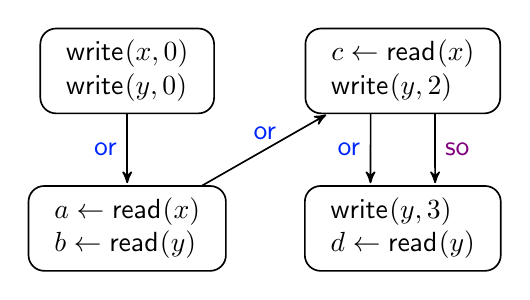
\begin{tikzpicture}[->,>=stealth',shorten >=1pt,auto,node distance=3cm,
				semithick, transform shape]
				\node[draw, rounded corners=2mm,outer sep=0] (t1) at (-3.5, 0) {\begin{tabular}{l} 
						$\wrt{x}{0}$ \\
						$\wrt{y}{0}$
				\end{tabular}};
				
				\node[draw, rounded corners=2mm,outer sep=0] (t2) at (-3.5, -2) {
					\begin{tabular}{l}
						$a \gets \rd{x}$ \\
						$b \gets \rd{y}$						
				\end{tabular}};
				
				\node[draw, rounded corners=2mm,outer sep=0] (t3) at (0, 0) {
					\begin{tabular}{l}
						$c \gets \rd{x}$ \\
						$\wrt{y}{2}$
				\end{tabular}};
				
				\node[draw, rounded corners=2mm,outer sep=0] (t4) at (0, -2) {
					\begin{tabular}{l} 
						$\wrt{y}{3}$ \\
						$d \gets \rd{y}$
				\end{tabular}};
				
				\path (t1) edge[left] node[yshift=0,xshift=0] {$\ora$} (t2);
				\path (t2) edge[above] node[yshift=0,xshift=0] {$\ora$} (t3);
				
				\path (t3.south east) -- (t3.south) coordinate[pos=0.67] (t3so);
				\path (t3.south west) -- (t3.south) coordinate[pos=0.67] (t3or);
				\path (t4.north east) -- (t4.north) coordinate[pos=0.67] (t4so);
				\path (t4.north west) -- (t4.north) coordinate[pos=0.67] (t4or);
				\path (t3or) edge[left] node[yshift=0,xshift=0] {$\ora$} (t4or);
				\path (t3so) edge[right] node[yshift=0,xshift=0] {$\so$} (t4so);
			\end{tikzpicture}  
			
		}
		\caption{$\ora$ produce a total order between all transactions in the program.}
		\label{fig:oracle_order:a}
	\end{subfigure}
	\hspace{.7cm}
	\centering
	\begin{subfigure}[b]{.32\textwidth}
		\resizebox{\textwidth}{!}{
			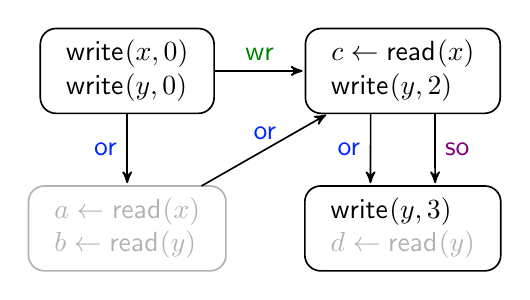
\begin{tikzpicture}[->,>=stealth',shorten >=1pt,auto,node distance=3cm,
				semithick, transform shape]
				\node[draw, rounded corners=2mm,outer sep=0] (t1) at (-3.5, 0) {\begin{tabular}{l} 
						$\wrt{x}{0}$ \\
						$\wrt{y}{0}$
				\end{tabular}};
				
				\node[draw, rounded corners=2mm,outer sep=0, opacity=0.3] (t2) at (-3.5, -2) {
					\begin{tabular}{l}
						$a \gets \rd{x}$ \\
						$b \gets \rd{y}$						
				\end{tabular}};
				
				\node[draw, rounded corners=2mm,outer sep=0] (t3) at (0, 0) {
					\begin{tabular}{l}
						$c \gets \rd{x}$ \\
						$\wrt{y}{2}$
				\end{tabular}};
				
				\node[draw, rounded corners=2mm,outer sep=0] (t4) at (0, -2) {
					\begin{tabular}{l} 
						$\wrt{y}{3}$ \\
						{\pgfsetfillopacity{0.3}$d \gets \rd{y}$}
				\end{tabular}};
				
				\path (t1) edge[left] node[yshift=0,xshift=0] {$\ora$} (t2);
				\path (t2) edge[above] node[yshift=0,xshift=0] {$\ora$} (t3);
				\path (t1) edge[above] node[yshift=0,xshift=0] {$\wro$} (t3);
				
				\path (t3.south east) -- (t3.south) coordinate[pos=0.67] (t3so);
				\path (t3.south west) -- (t3.south) coordinate[pos=0.67] (t3or);
				\path (t4.north east) -- (t4.north) coordinate[pos=0.67] (t4so);
				\path (t4.north west) -- (t4.north) coordinate[pos=0.67] (t4or);
				\path (t3or) edge[left] node[yshift=0,xshift=0] {$\ora$} (t4or);
				\path (t3so) edge[right] node[yshift=0,xshift=0] {$\so$} (t4so);
			\end{tikzpicture}  
			
		}
		\caption{An incomplete history and its $\ora$ order.}
		\label{fig:oracle_order:b}
	\end{subfigure}
	\caption{Some possible oracle order between transactions. TODO MAY NEED TO EXPLAIN THE CONVENTIONS IN THE PICTURE.}
	\label{fig:oracle_order}
	
\end{figure}

TODO: THIS SHOULD BE AN EXAMPLE OF A STEP OF NEXT. ADD TO THE ABOVE EXAMPLE SOME LOCAL INSTRUCTION BEFORE THE READ(Y), AND TALK ABOUT LOCAL STATES AS WELL. ALSO, ON THE LEFT, PUT THE PROGRAM AND NOT A HISTORY (PROGRAM WRITTEN WITH THE SYNTAX PRESENTED AT THE BEGINNING OF THE PAPER).

For example, given the history $h$ in Figure~\ref{fig:oracle_order:b}, the function $\nextEvent$ would return the event $d \gets \rd{y}$ instead of $a \gets \rd{x}$; as the forth transaction is pending in $h$. 

\begin{figure}[H]

\begin{subfigure}[b]{.25\textwidth}
%	\resizebox{\textwidth}{!}{
\begin{minipage}{1.8cm}
\begin{lstlisting}[xleftmargin=5mm,basicstyle=\ttfamily\scriptsize,escapeinside={(*}{*)}]
begin;
write((*$x$*),1);
write((*$y$*),1);
commit
\end{lstlisting}
\end{minipage}
\begin{minipage}{1mm}
||
\end{minipage}
\hspace{-5mm}
\begin{minipage}{1.3cm}
\begin{lstlisting}[xleftmargin=5mm,basicstyle=\ttfamily\scriptsize,escapeinside={(*}{*)}]
begin;
a=read((*$x$*));
b=read((*$y$*));
commit
begin;
c=read((*$x$*));
commit
\end{lstlisting}
\end{minipage}
%		}
\caption{Program.}
\label{fig:add_read:prog}
\end{subfigure}
	\centering
	\begin{subfigure}[b]{.2\textwidth}
		\resizebox{\textwidth}{!}{
			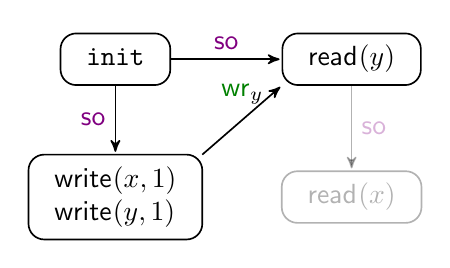
\begin{tikzpicture}[->,>=stealth',shorten >=1pt,auto,node distance=3cm,
				semithick, transform shape]
				\node[draw, rounded corners=2mm,outer sep=0] (t1) at (-3, 0) {\begin{tabular}{l} $\init$\end{tabular}};
				\node[draw, rounded corners=2mm,outer sep=0] (t2) at (-3, -1.75) {\begin{tabular}{l} $\wrt{x}{1}$ \\ $\wrt{y}{1}$ \end{tabular}};
				\node[draw, rounded corners=2mm,outer sep=0] (t3) at (0, 0) {\begin{tabular}{l} $\rd{y}$\end{tabular}};
				\node[draw, rounded corners=2mm, outer sep=0, opacity=0.3] (t4) at (0, -1.75) {
					\begin{tabular}{l} 
					$\rd{x}$
				\end{tabular}};
				
				\path (t1.south east) -- (t1.east) coordinate[pos=0.67] (t1y);
				\path (t1.north east) -- (t1.east) coordinate[pos=0.67] (t1x);
				\path (t3.south west) -- (t3.west) coordinate[pos=0.67] (t3y);
				\path (t3.north west) -- (t3.west) coordinate[pos=0.67] (t3x);
				%\path (t1x) edge[above] node[yshift=0,xshift=0] {$\wro_x$} (t3x);
				\path (t1.east) edge[above] node[yshift=0,xshift=0] {$\so$} (t3.west);
				\path (t1.south) edge[above] node[left] {$\so$} (t2.north);
				\path (t2.north east) edge[above] node [yshift=2,xshift=0] {$\wro_y$} (t3.south west);
				\path[opacity=0.3] (t3.south) edge[below] node [right]{$\so$} (t4.north); %[yshift=0,xshift=0]
			\end{tikzpicture}  
			
		}
		\caption{Current history.}
		\label{fig:add_read:a}
	\end{subfigure}
	\hspace{.5cm}
	\centering
	\begin{subfigure}[b]{.2\textwidth}
		\resizebox{\textwidth}{!}{
			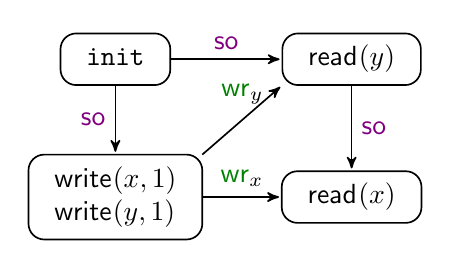
\begin{tikzpicture}[->,>=stealth',shorten >=1pt,auto,node distance=3cm,
				semithick, transform shape]
				\node[draw, rounded corners=2mm,outer sep=0] (t1) at (-3, 0) {\begin{tabular}{l} $\init$\end{tabular}};
				\node[draw, rounded corners=2mm,outer sep=0] (t2) at (-3, -1.75) {\begin{tabular}{l} $\wrt{x}{1}$ \\ $\wrt{y}{1}$ \end{tabular}};
				\node[draw, rounded corners=2mm,outer sep=0] (t3) at (0, 0) {\begin{tabular}{l} $\rd{y}$\end{tabular}};
				\node[draw, rounded corners=2mm, outer sep=0] (t4) at (0, -1.75) {
					\begin{tabular}{l} 
						$\rd{x}$
				\end{tabular}};
				
				\path (t1.south east) -- (t1.east) coordinate[pos=0.67] (t1y);
				\path (t1.north east) -- (t1.east) coordinate[pos=0.67] (t1x);
				\path (t3.south west) -- (t3.west) coordinate[pos=0.67] (t3y);
				\path (t3.north west) -- (t3.west) coordinate[pos=0.67] (t3x);
				%\path (t1x) edge[above] node[yshift=0,xshift=0] {$\wro_x$} (t3x);
				\path (t1.east) edge[above] node[yshift=0,xshift=0] {$\so$} (t3.west);
				\path (t1.south) edge[above] node[left] {$\so$} (t2.north);
				\path (t2.north east) edge[above] node [yshift=2,xshift=0] {$\wro_y$} (t3.south west);
				\path (t3.south) edge[below] node [right]{$\so$} (t4.north);
				\path (t2.east) edge[below] node [above]{$\wro_x$} (t4.west); %[yshift=0,xshift=0] %[yshift=0,xshift=0]
			\end{tikzpicture}  
			
		}
		\caption{One extension.}
		\label{fig:add_read:b}
	\end{subfigure}\hspace{.5cm}
	\centering
	\begin{subfigure}[b]{.2\textwidth}
		\resizebox{\textwidth}{!}{
			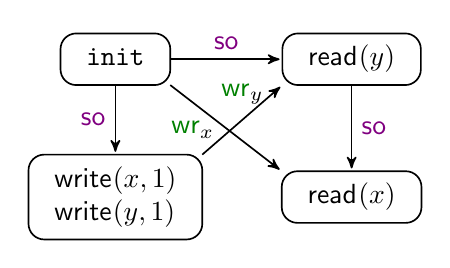
\begin{tikzpicture}[->,>=stealth',shorten >=1pt,auto,node distance=3cm,
				semithick, transform shape]
				\node[draw, rounded corners=2mm,outer sep=0] (t1) at (-3, 0) {\begin{tabular}{l} $\init$\end{tabular}};
				\node[draw, rounded corners=2mm,outer sep=0] (t2) at (-3, -1.75) {\begin{tabular}{l} $\wrt{x}{1}$ \\ $\wrt{y}{1}$ \end{tabular}};
				\node[draw, rounded corners=2mm,outer sep=0] (t3) at (0, 0) {\begin{tabular}{l} $\rd{y}$\end{tabular}};
				\node[draw, rounded corners=2mm, outer sep=0] (t4) at (0, -1.75) {
					\begin{tabular}{l} 
						$\rd{x}$
				\end{tabular}};
				
				\path (t1.south east) -- (t1.east) coordinate[pos=0.67] (t1y);
				\path (t1.north east) -- (t1.east) coordinate[pos=0.67] (t1x);
				\path (t3.south west) -- (t3.west) coordinate[pos=0.67] (t3y);
				\path (t3.north west) -- (t3.west) coordinate[pos=0.67] (t3x);
				%\path (t1x) edge[above] node[yshift=0,xshift=0] {$\wro_x$} (t3x);
				\path (t1.east) edge[above] node[yshift=0,xshift=0] {$\so$} (t3.west);
				\path (t1.south) edge[above] node[left] {$\so$} (t2.north);
				\path (t2.north east) edge[above] node [yshift=2,xshift=0] {$\wro_y$} (t3.south west);
				\path (t3.south) edge[below] node [right]{$\so$} (t4.north);
				\path (t1.south east) edge[below] node [yshift=6,xshift=-12]{$\wro_x$} (t4.north west); %[yshift=0,xshift=0] %[yshift=0,xshift=0]
			\end{tikzpicture}  
			
		}
		\caption{Another extension.}
		\label{fig:add_read:c}
	\end{subfigure}\hspace{.5cm}
	\caption{Extensions of a history by adding a $\iread$ event. TODO MAY NEED TO EXPLAIN THE CONVENTIONS IN THE PICTURE.}
	\label{fig:add_read}
	%\vspace{-3mm}
\end{figure}

%TODO REDO THE ABOVE FIGURE IN THE SPIRIT OF FIGURE \ref{fig:dead_branch}. MODIFY THE EXAMPLE SO ONE OF THE TWO CHOICES DOES NOT SATISFY SOME ISOLATION LEVEL, TO EXEMPLIFY THE USE OF $\genericValidWrites$.

If the event returned by $\genericNext$ is not a read event, then it is simply added to the current history, as the maximal element of the order $<$ (cf. the definition of $\oplus_j$ on ordered histories). If it is a read event, then adding this event may result in multiple histories depending on the associated $\wro$ dependency. 
%
%The incremental process of obtaining histories with more information it is called \textit{extension}. In essence, given a history $h$ and an event $e \not\in h$, all possible graphs using these two elements must be constructed. 
%If $e$'s type is $\ibegin$ or $\iend$, there is only one possible way to extend it by the operator $\bullet$'s definition. When $e$ is a $\iread$, however, we have to explore multiple histories, one per $\wro$-dependency that can be generated with a $\iwrite$ event $w\in h$ and $e$. That is, all histories $h \bullet_w e$. 
For example, in Figure \ref{fig:add_read}, extending the history in Figure \ref{fig:add_read:a} with the $\erd{x}$ event could result in two different histories, pictured in Figure \ref{fig:add_read:b} and \ref{fig:add_read:c}, depending on the write with whom this read event is associated by $\wro$. However, under $\CC$, the latter history is inconsistent.
%we can obtain two different histories depending on the $\wro$ dependency created (figures \ref{fig:add_read:b} and \ref{fig:add_read:c}). In both three cases, we declare the algorithm order for this new history $h'$ by simply juxtaposing $e$ to all the previous ones: $\leq_{h'} = \leq_h \cup \{\langle e', e \rangle \ | \  e' \in h\}$.
The function $\genericValidWrites$ limits the choices to those that preserve consistency with the intended isolation level $I$, i.e.,
%However, we will only select those $\iwrite$ event such that the extended history $h \bullet_w e$ is consistent, as described by function $\validWrites$; which will eventually play the $\genericValidWrites$'s role in our algorithm.  

\begin{cframed}[pinegreen]
	\begin{equation*}
		\begin{array}{ccc}
			\genericValidWrites(h, e) & \coloneqq & \{w \ | \ h \oplus_j e \oplus \wro(w,e) \mbox{ satisfies }I\}
		\end{array}
	\end{equation*}
\end{cframed}


%Finally, we declare the function $\evaluate$ that detects when a history is total.
%
%\begin{cframed}[pinegreen]
%	\begin{equation*}
%		\begin{array}{ccc}
%			\evaluate(h) & \coloneqq & \nextEvent(h) = \bot
%		\end{array}
%	\end{equation*}
%\end{cframed}

%Nevertheless, we will guarantee in both cases that every possible incomplete history will be $\so$-bounded, i.e. if $e \ [\so \cup \po]^+ e'$ and $e' \in h$ then $e \in h$; in order to easily avoid eventual inconsistencies. Therefore, the global order $\ora$ presented in Figure~\ref{fig:oracle_order:a} restrict in a simple but effective way the duplicity between histories: the order events are being added don't cause \textit{per se} redundancies.%In the second case, to avoid randomness, we will have a function $\nextEvent$ that given a history $h$ returns the first event $e$ according to $\ora$ that is not in $h$; to obtain the new history $h' = h \bullet e$. For example, given the history in Figure~\ref{fig:oracle_order:b}, the function $\nextEvent$ would return the event $\ibegin$ associated to the second transaction. Nevertheless, we will guarantee in both cases that every possible incomplete history will be $\so$-bounded, i.e. if $e \ [\so \cup \po]^+ e'$ and $e' \in h$ then $e \in h$; in order to easily avoid eventual inconsistencies. Therefore, the global order $\ora$ presented in Figure~\ref{fig:oracle_order:a} restrict in a simple but effective way the duplicity between histories: the order events are being added don't cause \textit{per se} redundancies.

%Thanks to $\so$ and $\ora$ order, we will be able to track every possible history, and therefore, have control over the amount of graphs generated. 

%Incomplete histories can be extended in two ways: either with the extern help of some guide that select beforehand which events and in which order will be executed or without it. For managing the second case in a deterministic way, we will have a function $\nextEvent$ that maps every $h$ to some event that is not in $h$ for obtaining a new history $h' = h \bullet e$. If $h$ is incomplete and $l = \last{h}$ then $e$ is the minimum event in $\po_T$ bigger than $l$; but if not, $e$ is the $\ibegin$ event belonging to the minimal transaction $T$ according to $\ora$ that is not in $h$. For example, the function $\nextEvent$ would the history in Figure~\ref{fig:oracle_order:b} to the event $d \gets \rd{y}$. Clearly, any coherent history can be extended using $\nextEvent$ function resulting in a coherent history (as $\ora$ extends $\so$, it only suffices defining the $\wro$ edge that an eventual free $\iread$ would require).
%Nevertheless, we will guarantee in both cases that every possible incomplete history will be $\so$-bounded, i.e. if $e \ [\so \cup \po]^+ e'$ and $e' \in h$ then $e \in h$; in order to easily avoid eventual inconsistencies. Therefore, the global order $\ora$ presented in Figure~\ref{fig:oracle_order:a} restrict in a simple but effective way the duplicity between histories: the order events are being added don't cause \textit{per se} redundancies.%In the second case, to avoid randomness, we will have a function $\nextEvent$ that given a history $h$ returns the first event $e$ according to $\ora$ that is not in $h$; to obtain the new history $h' = h \bullet e$. For example, given the history in Figure~\ref{fig:oracle_order:b}, the function $\nextEvent$ would return the event $\ibegin$ associated to the second transaction. Nevertheless, we will guarantee in both cases that every possible incomplete history will be $\so$-bounded, i.e. if $e \ [\so \cup \po]^+ e'$ and $e' \in h$ then $e \in h$; in order to easily avoid eventual inconsistencies. Therefore, the global order $\ora$ presented in Figure~\ref{fig:oracle_order:a} restrict in a simple but effective way the duplicity between histories: the order events are being added don't cause \textit{per se} redundancies.

%!TEX root = main.tex
\subsection{Re-Ordering Events in Histories}
\label{subsection:SwappingHistories} %Provisional

After extending the current history with one more event, $\textsc{explore}$ may recurse on other histories obtained by re-ordering events in the current one (and dropping some other events).
%Besides sound and complete, we would also seek for an optimal algorithm, i.e. that avoids computing a history $h$ whose extensions are all inconsistent; also called a \textit{blocking} execution. If this is not achieved, our search would employ more resources such as time or memory than it actually needs for doing its purpose.

\begin{figure}[H]

	\centering
	\begin{subfigure}[b]{.25\textwidth}
		\begin{adjustbox}{max width=\textwidth}
	\begin{tabular}{c||c}
		\begin{lstlisting}[xleftmargin=5mm,basicstyle=\ttfamily\scriptsize,escapeinside={(*}{*)}, tabsize=1]
begin;
a = read((*x*));
b = read((*y*));
commit
		\end{lstlisting} &
		\begin{lstlisting}[xleftmargin=5mm,basicstyle=\ttfamily\scriptsize,escapeinside={(*}{*)}, tabsize=1]
begin;
write((*$x$*),2);
write((*$y$*),2);
commit
		\end{lstlisting} 
	\end{tabular} 
\end{adjustbox}
\vspace{1.2cm}
%		}
		\caption{Program.}
		\label{fig:dead_branch:prog}
	\end{subfigure}
\centering
	\begin{subfigure}[b]{.125\textwidth}
		\resizebox{\textwidth}{!}{
			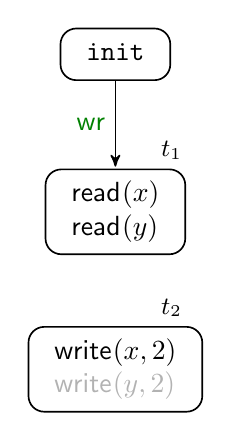
\begin{tikzpicture}[->,>=stealth',shorten >=1pt,auto,node distance=3cm,
				semithick, transform shape]
				
				%\\ \multicolumn{1}{c}{ \ldots}
				\node[draw, rounded corners=2mm,outer sep=0] (t1) at (-3.25, 0) {\begin{tabular}{l} $\init$ \end{tabular}};
				\node[draw, rounded corners=2mm,outer sep=0, label={[font=\small]50:$t_1$}] (t2) at (-3.25, -2) {\begin{tabular}{l} 
						$\rd{x}$ \\ $\rd{y}$
				\end{tabular}};
				\node[draw, rounded corners=2mm,outer sep=0, label={[font=\small]50:$t_2$}] (t3) at (-3.25, -4) {\begin{tabular}{l} 
						$\wrt{x}{2}$\pgfsetfillopacity{0.3}\\
						$\wrt{y}{2}$
				\end{tabular}};			
				
				\path (t1.south west) -- (t1.south) coordinate[pos=0.67] (t1x);
				\path (t1.south east) -- (t1.south) coordinate[pos=0.67] (t1y);
				\path (t2.north west) -- (t2.north) coordinate[pos=0.67] (t2x);
				\path (t2.north east) -- (t2.north) coordinate[pos=0.67] (t2y);
				
				\path (t1.south) edge [left] node {$\wro$} (t2.north);

				%\path (t2) edge [right] node {$\wro_x$} (t3);
			\end{tikzpicture}  
			
		}
		\caption{Current.}
		\label{fig:dead_branch:a}
	\end{subfigure}
	\hspace{.175cm}
	\centering
	\begin{subfigure}[b]{.125\textwidth}
		\resizebox{\textwidth}{!}{
			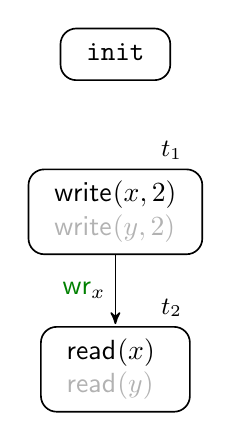
\begin{tikzpicture}[->,>=stealth',shorten >=1pt,auto,node distance=3cm,
				semithick, transform shape]
				\node[draw, rounded corners=2mm,outer sep=0] (t1) at (-3.25, 0) {\begin{tabular}{l} $\init$ \end{tabular}};
				\node[draw, rounded corners=2mm,outer sep=0, label={[font=\small]50:$t_2$}] (t2) at (-3.25, -4) {\begin{tabular}{l} 
						$\rd{x}$ \pgfsetfillopacity{0.3}\\ $\rd{y}$
				\end{tabular}};
				\node[draw, rounded corners=2mm,outer sep=0, label={[font=\small]50:$t_1$}] (t3) at (-3.25, -2) {\begin{tabular}{l} 
						$\wrt{x}{2}$\pgfsetfillopacity{0.3}\\
						$\wrt{y}{2}$
				\end{tabular}};			
				
				\path (t1.south west) -- (t1.south) coordinate[pos=0.67] (t1x);
				\path (t2.north west) -- (t2.north) coordinate[pos=0.67] (t2x);
				\path (t3.north west) -- (t3.west) coordinate[pos=0.67] (t3x);
				
				\path (t3.south) edge [left] node {$\wro_x$} (t2.north); %[yshift=8,xshift=0]
				%\path (t1x) edge [right] node {$\wro_y$} (t2x);
			\end{tikzpicture}  
			
		}
		\caption{Reorder.}
		\label{fig:dead_branch:b}
	\end{subfigure}
	\hspace{.175cm}
	\centering
		\begin{subfigure}[b]{.177\textwidth}
		\resizebox{\textwidth}{!}{
			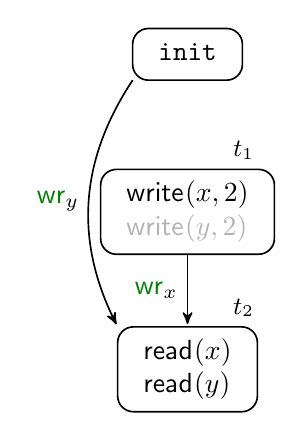
\begin{tikzpicture}[->,>=stealth',shorten >=1pt,auto,node distance=3cm,
				semithick, transform shape]
				\node[draw, rounded corners=2mm,outer sep=0] (t1) at (-3.25, 0) {\begin{tabular}{l} $\init$ \end{tabular}};
				\node[draw, rounded corners=2mm,outer sep=0, label={[font=\small]50:$t_2$}] (t2) at (-3.25, -4) {\begin{tabular}{l} 
						$\rd{x}$ \\ $\rd{y}$
				\end{tabular}};
				\node[draw, rounded corners=2mm,outer sep=0, label={[font=\small]50:$t_1$}] (t3) at (-3.25, -2) {\begin{tabular}{l} 
						$\wrt{x}{2}$\pgfsetfillopacity{0.3}\\
						$\wrt{y}{2}$
				\end{tabular}};			
				
				\path (t1.south west) -- (t1.south) coordinate[pos=0.67] (t1x);
				\path (t2.north west) -- (t2.north) coordinate[pos=0.67] (t2x);
				\path (t3.north west) -- (t3.west) coordinate[pos=0.67] (t3x);
				
				%\path (t3x) edge [above] node[yshift=8,xshift=0] {$\wro_x$} (t2.north east);
				\path (t3.south) edge [left] node {$\wro_x$} (t2.north);
				\path (t1.south west) edge [bend right] node[left] {$\wro_y$} (t2.north west);
			\end{tikzpicture}
		}
		\caption{Extended.}
		\label{fig:dead_branch:c}
	\end{subfigure}
	\hspace{.175cm}
	\centering
	\begin{subfigure}[b]{.177\textwidth}
		\resizebox{\textwidth}{!}{
			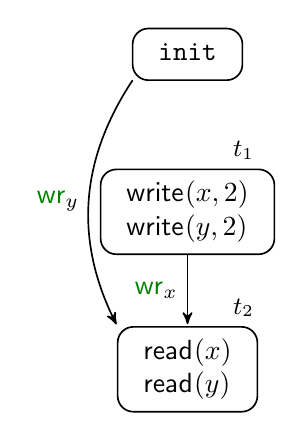
\begin{tikzpicture}[->,>=stealth',shorten >=1pt,auto,node distance=3cm,
				semithick, transform shape]
				\node[draw, rounded corners=2mm,outer sep=0] (t1) at (-3.25, 0) {\begin{tabular}{l} $\init$ \end{tabular}};
				\node[draw, rounded corners=2mm,outer sep=0, label={[font=\small]50:$t_2$}] (t2) at (-3.25, -4) {\begin{tabular}{l} 
						$\rd{x}$ \\ $\rd{y}$
				\end{tabular}};
				\node[draw, rounded corners=2mm,outer sep=0, label={[font=\small]50:$t_1$}] (t3) at (-3.25, -2) {\begin{tabular}{l} 
						$\wrt{x}{2}$\\
						$\wrt{y}{2}$
				\end{tabular}};			
				
				\path (t1.south west) -- (t1.south) coordinate[pos=0.67] (t1x);
				\path (t2.north west) -- (t2.north) coordinate[pos=0.67] (t2x);
				\path (t3.north west) -- (t3.west) coordinate[pos=0.67] (t3x);
				
				%\path (t3x) edge [above] node[yshift=8,xshift=0] {$\wro_x$} (t2.north east);
				\path (t3.south) edge [left] node {$\wro_x$} (t2.north);
				\path (t1.south west) edge [bend right] node[left] {$\wro_y$} (t2.north west);
			\end{tikzpicture}
			
		}
		\caption{Inconsistent.}
		\label{fig:dead_branch:d}
	\end{subfigure}
	\caption{Example of inconsistency after swapping two events. All $\so$-edges from $\init$ to the other transactions are omitted for legibility. All transaction logs are history-ordered top to bottom according to their position in the figure. Events in gray are not yet added to the history. }
	\label{fig:dead_branch}
	%\vspace{-3mm}
\end{figure}

%Proceeding this way we can ensure that every complete history is not inconsistent, but we cannot yet ensure every incomplete consistent history lead to a complete and consistent one. Guaranteeing it would mean that every step done in the algorithm is meaningful; that any explored branch would lead to a dead end. 
%The process of re-ordering events must maintain the invariant that the algorithm explores histories with at most one pending transaction, 
Re-ordering events must preserve the invariant of producing histories with at most one pending transaction.
To explain the use of this invariant in avoiding fruitless explorations, let us consider the program in Figure~\ref{fig:dead_branch:prog} assuming an exploration under Read Committed. The oracle order gives priority to the transaction on the left.
Assume that the current history reached by the exploration is the one pictured in Figure~\ref{fig:dead_branch:a} (the last added event is $\wrt{x}{2}$). Swapping the $\wrt{x}{2}$ event with the $\rd{x}$ event would result in the history pictured in Figure~\ref{fig:dead_branch:b}. To ensure that this swap produces a new history which was not explored in the past, the $\wro_x$ dependency of $\rd{x}$ is changed towards the $\wrt{x}{2}$ transaction (we detail this later).
%$\RA$
%One example of this undesired behavior can be easily seen under RA memory model with the program depicted in Figure~\ref{fig:dead_branch}. Here we consider three transactions ordered from left to right, top to bottom, and we start with the history depicted in Figure~\ref{fig:dead_branch:a}. After executing the $\nextEvent$ event, the $\iwrite$ $w_x  \coloneqq \wrt{x}{2}$, 
%one possible action would be swapping $w_x$ with the event $a \gets \rd{x}$; obtaining the history $h_2$ portrayed in Figure~\ref{fig:dead_branch:b}. 
By the definition of $\nextEvent$ (and the oracle order), this history shall be extended with $\rd{y}$, and this read event will be associated by $\wro_y$ to the only available $\iwrite(y,\_)$ event. This is pictured in 
Figure~\ref{fig:dead_branch:c}. The next exploration step will extend the history with $\ewrt{x,2}$ (the only extension possible) which however, results in a history that does \emph{not} satisfy Read Committed, thereby, the recursive exploration branch being blocked.
%as there is only one $\iwrite(y,\_)$ event, the $\wro$ dependncy for this
%that writes $y$, $r_b$ must read from the very first transaction; as seen in Figure~\ref{fig:dead_branch:c}. However, when completing the third transaction we must inexorably admit that our history in Figure~\ref{fig:dead_branch:d} is inconsistent. Therefore, all the computation required to complete the unfinished transactions after the swap was in vain; we couldn't detect after computing $h_2$ the dead end.
% As $\nextEvent$ function always prioritize pending transactions
The core issue is related to the history in Figure \ref{fig:dead_branch:c} which has a pending transaction that is \emph{not} $(\so \cup \wro)^*$-maximal. Being able to extend such a transaction while maintaining consistency with the intended isolation level is not guaranteed by Read Committed (and any other isolation level we consider). Nevertheless, causal extensibility guarantees the existence of an extension for pending transactions that are $(\so \cup \wro)^*$-maximal. We enforce this requirement by restricting the explored histories to have at most one pending transaction. This pending transaction will necessarily by $(\so \cup \wro)^*$-maximal.

%
%Hence, for being always able to extend a history by invoking the model's causally-extensibility, we have to never produce pending transactions that are non $\so \cup \wro$-maximal. A simple solution is always executing histories in isolation, i.e. having exactly one pending transaction; thus, $\so \cup \wro$-maximal,  otherwise there would be a previous point where two pending transactions coexisted. To sum up, we are not going to swap just after executing a $\iwrite$ event but when its transaction is completed.

%TODO EXPLAIN THE DEFINITIONS BELOW

To enforce histories with at most one pending transaction, the function $\genericCompute$, which identifies events to reorder, has a non-empty return value only when the last added event is $\ecommit$ (the end of a transaction). Therefore, in such a case, it returns pairs of read and write events on the same variable, the write event coming from the last completed transaction, and such that the transactions containing the two events are not causally dependent (i.e., related by $[\so \cup \wro]^*$).

\begin{cframed}[pinegreen]
	\begin{equation*}
		\begin{array}{lcl}
			\genericCompute(h_<) & \coloneqq & \{(r,w) \in \Events \ | \ r < w \land r \in \readOp{t} \land w \in \writeOp{t}\\[1mm]
			&& \hspace{1.9cm} \land\ \variable{r} = \variable{w} \\ [1mm]
			&& \hspace{1.9cm} \land\ (\trans{h}{r},t)\not\in [\so \cup \wro]^*\land \mbox{$t$ is complete}   \} \\[1mm]
			&& \mbox{where $t$ is the transaction log of the last event in $<$}
		\end{array}
	\end{equation*}
\end{cframed}

\begin{figure}[H]
\centering
\begin{subfigure}[b]{.25\textwidth}
	\begin{adjustbox}{max width=\textwidth}
		\begin{tabular}{c||c}
			\begin{lstlisting}[xleftmargin=5mm,basicstyle=\ttfamily\scriptsize,escapeinside={(*}{*)}, tabsize=1]
begin;
a = read((*x*));
write((*$y$*),1)
commit
begin;
b = read((*x*));
commit		
			\end{lstlisting} &
			\begin{lstlisting}[xleftmargin=5mm,basicstyle=\ttfamily\scriptsize,escapeinside={(*}{*)}, tabsize=1]
begin;
write((*$y$*),3);
commit
begin;
write((*$x$*),4);
commit
			\end{lstlisting} 
		\end{tabular} 
	\end{adjustbox}
	
	
	\caption{Program.}
	\label{fig:compute-reordering:prog}
\end{subfigure} 
\hspace{.15cm}%\pgfsetfillopacity{0.3}\\
	\centering
	\begin{subfigure}[b]{.2\textwidth}
		\resizebox{.81\textwidth}{!}{
			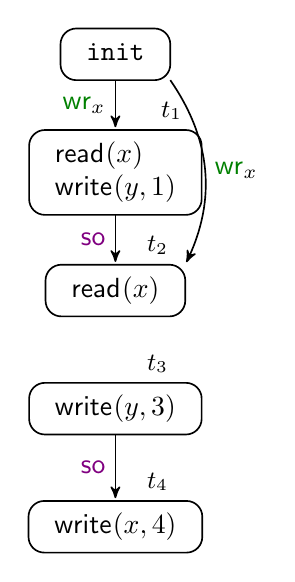
\begin{tikzpicture}[->,>=stealth',shorten >=1pt,auto,node distance=3cm,
				semithick, transform shape]
				
				%\\ \multicolumn{1}{c}{ \ldots}
				\node[draw, rounded corners=2mm,outer sep=0] (t0) at (0, 0) {\begin{tabular}{l} $\init$ \end{tabular}};
				\node[draw, rounded corners=2mm,outer sep=0, label={[font=\small]50:$t_1$}] (t1) at (0, -1.5) {\begin{tabular}{l} 
					$\rd{x}$ \\ $\wrt{y}{1}$ 
				\end{tabular}};
				\node[draw, rounded corners=2mm,outer sep=0, label={[font=\small]50:$t_2$}] (t2) at (0, -3) {\begin{tabular}{l} 
					$\rd{x}$
				\end{tabular}};
				\node[draw, rounded corners=2mm,outer sep=0, label={[font=\small]50:$t_3$}] (t3) at (0, -4.5) {\begin{tabular}{l} 
					$\wrt{y}{3}$
				\end{tabular}};
				\node[draw, rounded corners=2mm,outer sep=0, label={[font=\small]50:$t_4$}] (t4) at (0, -6) {\begin{tabular}{l} 
					$\wrt{x}{4}$
				\end{tabular}};			
				
				\path (t1.south west) -- (t1.south) coordinate[pos=0.67] (t1x);
				\path (t1.south east) -- (t1.south) coordinate[pos=0.67] (t1y);
				\path (t2.north west) -- (t2.north) coordinate[pos=0.67] (t2x);
				\path (t2.north east) -- (t2.north) coordinate[pos=0.67] (t2y);
				
				\path (t1.south) edge [left] node {$\so$} (t2.north);
				\path (t3.south) edge [left] node {$\so$} (t4.north);
				\path (t0.south) edge [left] node {$\wro_x$} (t1.north);\\
				\path (t0.south east) edge [bend left] node[right] {$\wro_x$} (t2.north east);
				
				%\path (t2) edge [right] node {$\wro_x$} (t3);
			\end{tikzpicture}  
			
		}
		\caption{Current.}
		\label{fig:compute-reordering:a}
	\end{subfigure}
	\hspace{.15cm}
	\centering
	\begin{subfigure}[b]{.2\textwidth}

		\resizebox{.77\textwidth}{!}{
			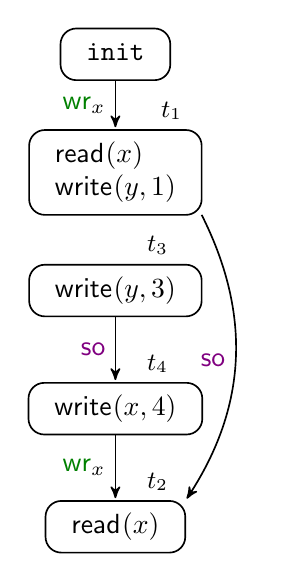
\begin{tikzpicture}[->,>=stealth',shorten >=1pt,auto,node distance=3cm,
				semithick, transform shape]
				\node[draw, rounded corners=2mm,outer sep=0] (t0) at (0, 0) {\begin{tabular}{l} $\init$ \end{tabular}};
				\node[draw, rounded corners=2mm,outer sep=0, label={[font=\small]50:$t_1$}] (t1) at (0, -1.5) {\begin{tabular}{l} 
						$\rd{x}$ \\ $\wrt{y}{1}$ 
				\end{tabular}};
				\node[draw, rounded corners=2mm,outer sep=0, label={[font=\small]50:$t_2$}] (t2) at (0, -6) {\begin{tabular}{l} 
						$\rd{x}$
				\end{tabular}};
				\node[draw, rounded corners=2mm,outer sep=0, label={[font=\small]50:$t_3$}] (t3) at (0, -3) {\begin{tabular}{l} 
						$\wrt{y}{3}$
				\end{tabular}};
				\node[draw, rounded corners=2mm,outer sep=0, label={[font=\small]50:$t_4$}] (t4) at (0, -4.5) {\begin{tabular}{l} 
						$\wrt{x}{4}$
				\end{tabular}};			
				
				\path (t1.south west) -- (t1.south) coordinate[pos=0.67] (t1x);
				\path (t1.south east) -- (t1.south) coordinate[pos=0.67] (t1y);
				\path (t2.north west) -- (t2.north) coordinate[pos=0.67] (t2x);
				\path (t2.north east) -- (t2.north) coordinate[pos=0.67] (t2y);
				
				\path (t1.south east) edge [bend left] node [left] {$\so$} (t2.north east);
				\path (t3.south) edge [left] node {$\so$} (t4.north);
				\path (t0.south) edge [left] node {$\wro_x$} (t1.north);\\
				\path (t4.south) edge [left] node{$\wro_x$} (t2.north);
				 %[yshift=8,xshift=0]
				%\path (t1x) edge [right] node {$\wro_y$} (t2x);
			\end{tikzpicture}  

		}
		
				\caption{Swap $t_2$ and $t_4$.}
	
		\label{fig:compute-reordering:b}
	\end{subfigure}
	\hspace{.15cm}
	\centering
	\begin{subfigure}[b]{.2\textwidth}
		\resizebox{.6\textwidth}{!}{
				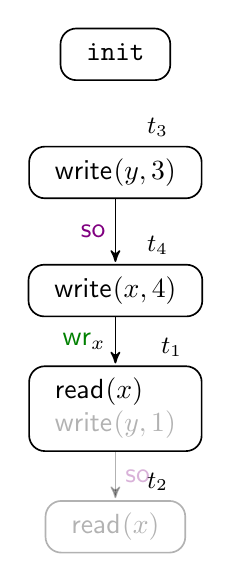
\begin{tikzpicture}[->,>=stealth',shorten >=1pt,auto,node distance=3cm,
				semithick, transform shape]
				\node[draw, rounded corners=2mm,outer sep=0] (t0) at (0, 0) {\begin{tabular}{l} $\init$ \end{tabular}};
				\node[draw, rounded corners=2mm,outer sep=0, label={[font=\small]50:$t_1$}] (t1) at (0, -4.5) {\begin{tabular}{l} 
						$\rd{x}$ \\ \pgfsetfillopacity{0.3}$\wrt{y}{1}$ 
				\end{tabular}};
				\node[draw, rounded corners=2mm,outer sep=0, opacity=0.3, label={[font=\small]50:$t_2$}] (t2) at (0, -6) {\begin{tabular}{l} 
						$\rd{x}$
				\end{tabular}};
				\node[draw, rounded corners=2mm,outer sep=0, label={[font=\small]50:$t_3$}] (t3) at (0, -1.5) {\begin{tabular}{l} 
						$\wrt{y}{3}$
				\end{tabular}};
				\node[draw, rounded corners=2mm,outer sep=0, label={[font=\small]50:$t_4$}] (t4) at (0, -3) {\begin{tabular}{l} 
						$\wrt{x}{4}$
				\end{tabular}};			
				
				\path (t1.south west) -- (t1.south) coordinate[pos=0.67] (t1x);
				\path (t1.south east) -- (t1.south) coordinate[pos=0.67] (t1y);
				\path (t2.north west) -- (t2.north) coordinate[pos=0.67] (t2x);
				\path (t2.north east) -- (t2.north) coordinate[pos=0.67] (t2y);
				
				\path[opacity=0.3] (t1.south) edge [left] node [right] {$\so$} (t2.north);
				\path (t3.south) edge [left] node {$\so$} (t4.north);
				\path (t4.south) edge [left] node {$\wro_x$} (t1.north);\\
				%\path (t4.south) edge [left] node{$\wro_x$} (t2.north);
				%[yshift=8,xshift=0]
				%\path (t1x) edge [right] node {$\wro_y$} (t2x);
			\end{tikzpicture}  
			
		}
		\caption{Swap $t_1$ and $t_4$.}
		\label{fig:compute-reordering:c}
	\end{subfigure}
	\caption{Example of inconsistency after swapping two events. All $\so$-edges from $\init$ to the other transactions are omitted for legibility. All transaction logs are history-ordered top to bottom according to their position in the figure. Events in gray are not yet added to the history.}
	\label{fig:compute-reordering}
	%\vspace{-3mm}
\end{figure}

For example, given the program in Figure~\ref{fig:compute-reordering:prog} and history $h$ in Figure~\ref{fig:compute-reordering:b}, $\compute(h)$ would return $(r_1, t_4)$ and $(r_2, t_4)$ where $r_1$ and $r_2$ are the event $\rd{x}$ both belonging to $t_1$ and $t_2$ respectively.

Given a pair $(r,w)$, the function $\genericSwap$ produces a new history $\hist'$ which contains all events ordered before $r$ (w.r.t. $<$), the transaction that contains $w$ and all its $[\so \cup \wro]^*$ predecessors, and the event $r$ reading from $w$. Note that the $\po$ predecessors of $r$ from the same transaction are ordered before $r$ by $<$ and they will be also included in $\hist'$. More generally, the history $\hist'$ without $r$ is a prefix of the input history $\hist$. By definition, the only pending transaction in $\hist'$ is the one containing the read $r$. The order relation is updated by moving the transaction containing the read $r$ to be the last; it remains unchanged for the rest of the events.

\begin{cframed}[pinegreen]
	\begin{equation*}
		\begin{array}{lcl}
			\genericSwap(h_<, r, w, \locals) & \coloneqq &\big(h' = (h \setminus D) \oplus \wro(w,r), <'\big ), \locals', \text{ where} \\[1mm]
			&& \hspace{1cm}D = \{e \ | \ r < e \land (\trans{h}{e},\trans{h}{w})\not\in [\so \cup \wro]^*\} \\[1mm]
			&& \hspace{1cm}<' = \big( <\ \downarrow\ (\events{h'}\setminus \events{\trans{h'}{r}}) \big) \cdot \trans{h'}{r} \\[1mm]
			&& \hspace{1cm}\mbox{$\locals' = \locals \downarrow \events{h'}$.}
		\end{array}
	\end{equation*}
\end{cframed}

Above, $h \setminus D$ denotes the prefix of $\hist$ obtained by deleting all the events in $D$ from its transaction logs; a transaction log is removed all together if it becomes empty. Also, $\hist'' \oplus \wro(w,r)$ denotes an \emph{update} of the $\wro$ relation of $\hist''$ where any pair $(\_,r)$ is replaced by $(w,r)$. Finally, $<'' \cdot\ \trans{h'}{r}$ denotes an extension of the total order $<''$ obtained by appending the events in $\trans{h'}{r}$ according to program order.

Continuing with the example of Figure~\ref{fig:compute-reordering}, while swapping $t_1$ and $t_4$, every event in transaction $t_2$ and $\wrt{y}{1}$ in $t_1$ belong to $\{e \ | \ r < e \land (\trans{h}{e},\trans{h}{w})\not\in [\so \cup \wro]^*\}$, so it will not belong to the swapped history; as it can be seen in Figure~\ref{fig:compute-reordering:c}. If the other swap is done, no event but the commit in $t_2$ will be deleted (Figure~\ref{fig:compute-reordering:b}).

%Following algorithm \ref{algorithm:algo-class}'s schema, we define two functions $\compute, \swap$ that plays the role of $\genericCompute, \genericSwap$ respectively. In addition, for the history $h' = \swap(h, r, w)$ we declare the algorithm order of $h'$, $\leq_{h'}$ as $\leq_{h'} = \leq_{(h \setminus \tr(r) ) \restriction_{h'}} \cup \{\langle e, e' \rangle \ | \ e \in h' \setminus \tr(r), e' \in \tr(r)\} \cup \po_{\tr(r) \restriction_{h'}}$.
%
%\begin{cframed}[pinegreen]
%	\begin{equation*}
%		\begin{array}{ccc}
%			\compute(h) & \coloneqq & \{(r,w) \in h^2 \ | \ r <_h w \land \variable{r} = \variable{w} \land w \in \tr(\last{h}) \} \\
%			\swap(h, r, w) & \coloneqq & (h \setminus D) \bullet_w r \\
%			& \text{where} & D = \{e \ | \ r \leq_h e \land \lnot (\tr(e) \ [\so \cup \wro]^* \ \tr(w))\}
%		\end{array}
%	\end{equation*}
%\end{cframed}


\subsection{Avoiding Redundancy}

%Conversely, adding a $\iwrite$ $w$ is more complicated, multiple events may read this new event; specifically. the number of possible histories is exponential, $2^{|\iread(h)|}$. Moreover, after changing a $\wro$-edge from a $\iread$ $r$, we have no knowledge of the rest of the event's presence: some conditional instruction may be executed after $r$ and it may be meaningless talking about them. Thus, checking for every possible set of $\iread$ events if reading from $w$ leads to something consistent is no reasonable. Therefore, we have to define a criterion to determine whose sets of read events shall be analyzed. One hand, the history $h \bullet w$ where no $\iread$ reads from $w$ has to be explored, with an algorithm order defined in an analogously as for any other aforementioned history. On the other hand, we select one $\iread$ $r$ that will be the first event in $h$ reading from $w$ while the ones that follow $r$ will have to be re-executed. As $r$ had already been executed, what at the end we produce is a swap between the relative orders of $r$ and $w$; so $r$ would be thereinafter called \textit{swapped}.

%As in a more formal way definition \ref{def:swapped} states, this read $r$ would be thereinafter called \textit{swapped}

%Moreover, after changing a $\wro$-edge, we have no knowledge of the rest of the event's presence: some conditional instruction may be executed after that $\iread$ and it may be meaningless talking about the rest of the events. Moreover, by the prefix-closedness of our model, an inconsistent history only leads to inconsistent ones; so there is no reasonable reason for exploring those. Thus, instead of generating every single one of them and check afterwards if they are consistent, we prefer to generate a small subset and only extends those ones that are consistent; by the prefix-closedness of our model, an inconsistent history only leads to inconsistent ones. %Therefore, we can detect inconsistencies early on.

%Our protocol is defined as follows: we will select one $\iread$ event that will be the first event in $h$ reading from $w$ while the ones that proceed $r$ will be marked as postponed; they will have to be re-executed. As in a more formal way definition \ref{def:swapped} states, This read $r$ would be thereinafter called \textit{swapped}:

%, and we will enforce the following properties: no event before $r$ will read from $w$, $r$ reads from $w$, every read after $r$ may or may not read from $w$. 



While extending histories according to $\genericNext$ and recursing on re-ordered histories whenever possible (taking $\genericProtocol$ as $\mathit{true}$) guarantees soundness and completeness, it does not guarantee optimality. There are two sources of redundancy in this trivial algorithm: (1) re-ordering the same read multiple times, and (2) applying $\genericSwap$ on different histories may give the same result.

\begin{figure}[h]
	
\begin{subfigure}[b]{.3\textwidth}
\begin{adjustbox}{max width=\textwidth}
\begin{tabular}{c||c}
	\begin{lstlisting}[xleftmargin=5mm,basicstyle=\ttfamily\scriptsize,escapeinside={(*}{*)}, tabsize=1]
begin;
a=read((*$x$*));
commit
	\end{lstlisting} &
	\begin{lstlisting}[xleftmargin=5mm,basicstyle=\ttfamily\scriptsize,escapeinside={(*}{*)}, tabsize=1]
begin;
b=read((*$y$*));
commit
	\end{lstlisting} 

\\
\multicolumn{1}{c}{} & \multicolumn{1}{c}{}
\\
	\begin{lstlisting}[xleftmargin=5mm,basicstyle=\ttfamily\scriptsize,escapeinside={(*}{*)}, tabsize=1]
begin;
write((*$y$*),3);
commit
	\end{lstlisting} &
	\begin{lstlisting}[xleftmargin=5mm,basicstyle=\ttfamily\scriptsize,escapeinside={(*}{*)}, tabsize=1]
begin;
write((*$x$*),4);
commit
	\end{lstlisting}
\end{tabular} 
\end{adjustbox}

\caption{Program.}
\label{fig:redundant_Swap:prog}
\end{subfigure}
	\centering
	\begin{subfigure}[b]{.21\textwidth}
		\resizebox{.6\textwidth}{!}{
			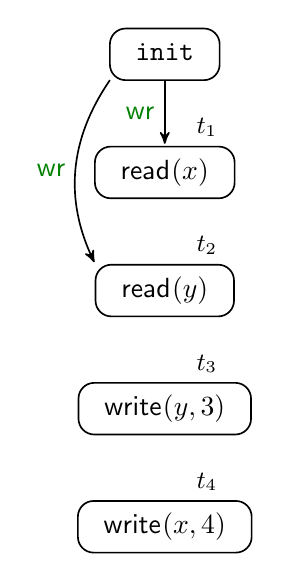
\begin{tikzpicture}[->,>=stealth',shorten >=1pt,auto,node distance=3cm,
				semithick, transform shape]
				\node[draw, rounded corners=2mm,outer sep=0] (t0) at (-3, 0) {\begin{tabular}{l} $\init$ \end{tabular}};
				
				\node[draw, rounded corners=2mm,outer sep=0, label={[font=\small]50:$t_1$}] (t1) at (-3, -1.5) {\begin{tabular}{l} $\rd{x}$\end{tabular}};
				\node[draw, rounded corners=2mm,outer sep=0, label={[font=\small]50:$t_2$}] (t2) at (-3, -3) {\begin{tabular}{l} $\rd{y}$  \end{tabular}};
				
				\node[draw, rounded corners=2mm,outer sep=0, label={[font=\small]50:$t_3$}] (t3) at (-3, -4.5) {\begin{tabular}{l} $\wrt{y}{3}$ \end{tabular}};
				\node[draw, rounded corners=2mm,outer sep=0, label={[font=\small]50:$t_4$}] (t4) at (-3, -6) {\begin{tabular}{l} $\wrt{x}{4}$ \end{tabular}};
				
				%\path (t0.south west) edge[above, bend right] node[left] {$\wro$} (t3.north west);
				\path (t0.south west) edge[above, bend right] node[left] {$\wro$} (t2.north west);
				\path (t0.south) edge node[left] {$\wro$} (t1.north);
				%\path (t0.south east) edge[above, bend left] node[left] {$\wro$} (t4.north east);
			\end{tikzpicture}  
		}
		\caption{Current history.}
		\label{fig:redundant_swap:a}
	\end{subfigure}
	\hspace{.25cm}
	\centering
	\begin{subfigure}[b]{.21\textwidth}
		\resizebox{.63\textwidth}{!}{
			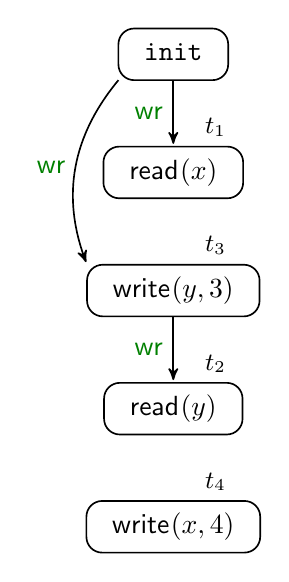
\begin{tikzpicture}[->,>=stealth',shorten >=1pt,auto,node distance=3cm,
				semithick, transform shape]
				\node[draw, rounded corners=2mm,outer sep=0] (t0) at (-3, 0) {\begin{tabular}{l} $\init$ \end{tabular}};
				
				\node[draw, rounded corners=2mm,outer sep=0, label={[font=\small]50:$t_1$}] (t1) at (-3, -1.5) {\begin{tabular}{l} $\rd{x}$ \end{tabular}};
				\node[draw, rounded corners=2mm,outer sep=0, label={[font=\small]50:$t_2$}] (t2) at (-3, -4.5) {\begin{tabular}{l} $\rd{y}$ \end{tabular}};
				
				\node[draw, rounded corners=2mm,outer sep=0, label={[font=\small]50:$t_3$}] (t3) at (-3, -3) {\begin{tabular}{l} $\wrt{y}{3}$ \end{tabular}};
				\node[draw, rounded corners=2mm,outer sep=0, label={[font=\small]50:$t_4$}] (t4) at (-3, -6) {\begin{tabular}{l} $\wrt{x}{4}$ \end{tabular}};
				
				\path (t0.south west) edge[above, bend right] node[left] {$\wro$} (t3.north west);
				\path (t3.south) edge node[left] {$\wro$} (t2.north);
				\path (t0.south) edge node[left] {$\wro$} (t1.north);
				%\path (t0.south east) edge[above, bend left] node[left] {$\wro$} (t4.north east);
			\end{tikzpicture}  
		}
		
		\caption{Swap $t_2$ and $t_3$.}
		\label{fig:redundant_swap:b}
	\end{subfigure}
	\hspace{.25cm}
	\centering
	\begin{subfigure}[b]{.21\textwidth}
		\resizebox{.65\textwidth}{!}{
			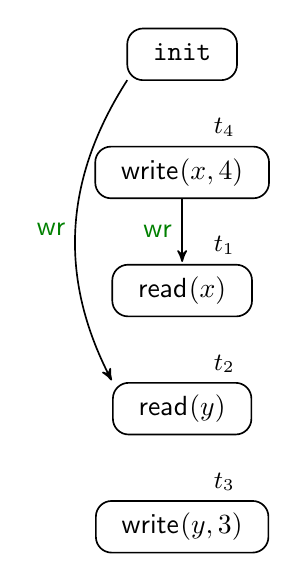
\begin{tikzpicture}[->,>=stealth',shorten >=1pt,auto,node distance=3cm,
				semithick, transform shape]
				\node[draw, rounded corners=2mm,outer sep=0] (t0) at (-3, 0) {\begin{tabular}{l} $\init$ \end{tabular}};
				
				\node[draw, rounded corners=2mm,outer sep=0, label={[font=\small]50:$t_1$}] (t1) at (-3, -3) {\begin{tabular}{l} $\rd{x}$ \end{tabular}};
				\node[draw, rounded corners=2mm,outer sep=0, label={[font=\small]50:$t_2$}] (t2) at (-3, -4.5) {\begin{tabular}{l} $\rd{y}$ \end{tabular}};
				
				\node[draw, rounded corners=2mm,outer sep=0, label={[font=\small]50:$t_3$}] (t3) at (-3, -6) {\begin{tabular}{l} $\wrt{y}{3}$ \end{tabular}};
				\node[draw, rounded corners=2mm,outer sep=0, label={[font=\small]50:$t_4$}] (t4) at (-3, -1.5) {\begin{tabular}{l} $\wrt{x}{4}$ \end{tabular}};
				
				%\path (t0.south west) edge[above, bend right] node[left] {$\wro$} (t3.north west);
				\path (t0.south west) edge[above, bend right] node[left] {$\wro$} (t2.north west);
				\path (t4.south) edge node[left] {$\wro$} (t1.north);
				%\path (t0.south) edge node[left] {$\wro$} (t4.north);
			\end{tikzpicture}  
		}
		
		\caption{Swap $t_1$ and $t_4$.}
		\label{fig:redundant_swap:c}
	\end{subfigure}\hspace{.5cm}
	\caption{Two possible computable histories starting from a current one. The four transactions belong each one to a different independent thread.}
	\label{fig:redundant_swap}
	%\vspace{-3mm}
\end{figure}

For example, under the program depicted in Figure~\ref{fig:redundant_Swap:prog} with four independent threads, the algorithm may compute the history $h_1$ pictured in figure \ref{fig:redundant_swap:a}. Therefore, two different histories will also be computed via swapping two transactions: $h_2$ if we swap $t_2$ and $t_3$  (Figure~\ref{fig:redundant_swap:b}) and $h_3$ if we swap $t_1$ and $t_4$ (Figure~\ref{fig:redundant_swap:c}). However, from $h_2$ we can also swap $t_1$ and $t_4$ to produce a history that can be extended to $h_3$; obtaining twice the same history.


%TODO GIVE AN EXAMPLE FOR THE 1ST ISSUE. JUSTIFYING THE SWAPPED CONDITION. 

\begin{figure}[h]
	\begin{subfigure}[b]{.22\textwidth}
		\begin{adjustbox}{max width=\textwidth}
			\begin{tabular}{c||c}
				\begin{lstlisting}[xleftmargin=5mm,basicstyle=\ttfamily\scriptsize,escapeinside={(*}{*)}, tabsize=1]

begin;
write((*$x$*),2);
commit
				\end{lstlisting} &
				\begin{lstlisting}[xleftmargin=5mm,basicstyle=\ttfamily\scriptsize,escapeinside={(*}{*)}, tabsize=1]
begin;
a=read((*$x$*));
commit
				\end{lstlisting} 
				
				\\
				\multicolumn{1}{c}{} & \multicolumn{1}{c}{}
				\\
				\begin{lstlisting}[xleftmargin=5mm,basicstyle=\ttfamily\scriptsize,escapeinside={(*}{*)}, tabsize=1]
begin;
b=read((*$x$*));
commit
	\end{lstlisting} &
				\begin{lstlisting}[xleftmargin=5mm,basicstyle=\ttfamily\scriptsize,escapeinside={(*}{*)}, tabsize=1]
begin;
write((*$x$*),4);
commit
				\end{lstlisting}
			\end{tabular} 
		\end{adjustbox}
		
		\caption{Program.\\ $ $}
		\label{fig:non-optimality:prog}
	\end{subfigure}
	\centering
	\begin{subfigure}[b]{.15\textwidth}
		\resizebox{.95\textwidth}{!}{
			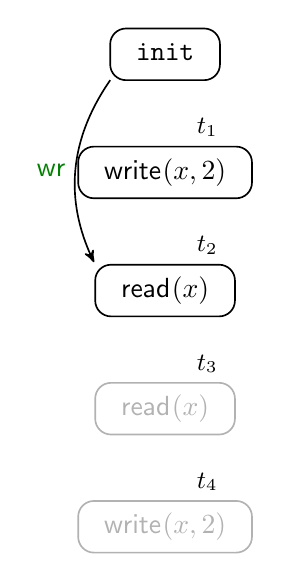
\begin{tikzpicture}[->,>=stealth',shorten >=1pt,auto,node distance=3cm,
				semithick, transform shape]
				\node[draw, rounded corners=2mm,outer sep=0] (t1) at (-3, 0) {\begin{tabular}{l} $\init$ \end{tabular}};
				
				\node[draw, rounded corners=2mm,outer sep=0, label={[font=\small]50:$t_1$}] (t2) at (-3, -1.5) {\begin{tabular}{l} $\wrt{x}{2}$ \end{tabular}};
				\node[draw, rounded corners=2mm,outer sep=0, label={[font=\small]50:$t_2$}] (t3) at (-3, -3) {\begin{tabular}{l} $\rd{x}$ \end{tabular}};
				
				\node[draw, rounded corners=2mm,outer sep=0, opacity=0.3, label={[font=\small]50:$t_3$}] (t4) at (-3, -4.5) {\begin{tabular}{l} $\rd{x}$ \end{tabular}};
				\node[draw, rounded corners=2mm,outer sep=0, opacity=0.3, label={[font=\small]50:$t_4$}] (t5) at (-3, -6) {\begin{tabular}{l} $\wrt{x}{2}$ \end{tabular}};
				
				\path (t1.south west) edge[above, bend right] node[left] {$\wro$} (t3.north west);
				%\path (-4.5,-3.75) edge[-,dashed] (-1,-3.75);
			\end{tikzpicture}  
			
		}
		\caption{Before reading.}
		\label{fig:non_optimality:a}
	\end{subfigure}
	\hspace{.15cm}
	\centering	
	\begin{subfigure}[b]{.15\textwidth}
		\resizebox{1.24\textwidth}{!}{
			\begin{tikzpicture}[->,>=stealth',shorten >=1pt,auto,node distance=3cm,
				semithick, transform shape]
				\node[draw, rounded corners=2mm,outer sep=0] (t1) at (-3, 0) {\begin{tabular}{l} $\init$ \end{tabular}};
				
				\node[draw, rounded corners=2mm,outer sep=0, label={[font=\small]50:$t_1$}] (t2) at (-3, -1.5) {\begin{tabular}{l} $\wrt{x}{2}$ \end{tabular}};
				\node[draw, rounded corners=2mm,outer sep=0, label={[font=\small]50:$t_2$}] (t3) at (-3, -3) {\begin{tabular}{l} $\rd{x}$ \end{tabular}};
				
				\node[draw, rounded corners=2mm,outer sep=0, label={[font=\small]50:$t_3$}] (t4) at (-3, -4.5) {\begin{tabular}{l} $\rd{x}$ \end{tabular}};
				
				\node[draw, rounded corners=2mm, opacity=0.3, label={[font=\small]50:$t_4$}] (t5) at (-3, -6) {\begin{tabular}{l} $\wrt{x}{4}$ \end{tabular}};
				
				%\path (t3) edge node {$\so$} (t5);
				%\path (t3) edge node {$\po$} (t3);
				%\path (t1) edge[below] node[yshift=-4,xshift=-4] {$\wro$} (t3_2);
				%\path (t2) edge[below] node[yshift=-4,xshift=4] {$\wro$} (t4_2);
%				\path (t1) edge[above] node[yshift=0,xshift=0] {$\wro$} (t3);
%				\path (t1) edge[below] node[yshift=-2,xshift=-2] {$\wro$} (t4);
				\path (t1.south west) edge[above, bend right] node[left] {$\wro$} (t3.north west);
				\path (t1.south east) edge[below, bend left] node[right] {$\wro$} (t4.north east);
				%\path (-4.5,-5.25) edge[-,dashed] (-1,-5.25);
			\end{tikzpicture}  
			
		}
		\caption{$t_3$ reads from $\init$.}
		\label{fig:non_optimality:b}
	\end{subfigure}
	\hspace{.15cm}
	\centering
	\begin{subfigure}[b]{.15\textwidth}
		\resizebox{1.24\textwidth}{!}{
			\begin{tikzpicture}[->,>=stealth',shorten >=1pt,auto,node distance=3cm,
				semithick, transform shape]
				\node[draw, rounded corners=2mm,outer sep=0] (t1) at (-3, 0) {\begin{tabular}{l} $\init$ \end{tabular}};
				
				\node[draw, rounded corners=2mm,outer sep=0, label={[font=\small]50:$t_1$}] (t2) at (-3, -1.5) {\begin{tabular}{l} $\wrt{x}{2}$ \end{tabular}};
				\node[draw, rounded corners=2mm,outer sep=0, label={[font=\small]50:$t_2$}] (t3) at (-3, -3) {\begin{tabular}{l} $\rd{x}$ \end{tabular}};
				
				\node[draw, rounded corners=2mm,outer sep=0, label={[font=\small]50:$t_3$}] (t4) at (-3, -4.5) {\begin{tabular}{l} $\rd{x}$ \end{tabular}};
				
				\node[draw, rounded corners=2mm, opacity=0.3, label={[font=\small]50:$t_4$}] (t5) at (-3, -6) {\begin{tabular}{l} $\wrt{x}{4}$ \end{tabular}};
				
				
				\path (t1.south west) edge[above, bend right] node[left] {$\wro$} (t3.north west);
				\path (t2.south east) edge[below, bend left] node[right] {$\wro$} (t4.north east);
				%\path (-4.5,-5.25) edge[-,dashed] (-1,-5.25);
			\end{tikzpicture}  
			
		}
		\caption{$t_3$ reads from $t_2$.}
		\label{fig:non_optimality:c}
	\end{subfigure}
	\hspace{.15cm}
	\centering
	\begin{subfigure}[b]{.15\textwidth}
		\resizebox{.75\textwidth}{!}{
			\begin{tikzpicture}[->,>=stealth',shorten >=1pt,auto,node distance=3cm,
				semithick, transform shape]
				\node[draw, rounded corners=2mm,outer sep=0] (t1) at (-3, 0) {\begin{tabular}{l} $\init$ \end{tabular}};
				\node[draw, rounded corners=2mm,outer sep=0, label={[font=\small]50:$t_1$}] (t2) at (-3, -1.5) {\begin{tabular}{l} $\wrt{x}{2}$ \end{tabular}};
				\node[draw, rounded corners=2mm,outer sep=0, label={[font=\small]50:$t_2$}] (t3) at (-3, -4.5) {\begin{tabular}{l} $\rd{x}$ \end{tabular}};
				
				\node[draw, rounded corners=2mm,outer sep=0, opacity=0.3, label={[font=\small]50:$t_3$}] (t4) at (-3, -6) {\begin{tabular}{l} $\rd{x}$ \end{tabular}};
				
				\node[draw, rounded corners=2mm, label={[font=\small]50:$t_4$}] (t5) at (-3, -3) {\begin{tabular}{l} $\wrt{x}{4}$ \end{tabular}};				
				
				\path (t5) edge[left] node {$\wro$} (t3);
				
			\end{tikzpicture}  
			
		}
		\caption{After swap.\\$ $}
		\label{fig:non_optimality:d}
	\end{subfigure}
	
	\caption{Re-ordering events versus optimality. We assume an oracle order orders transaction from left to right, top to bottom in the program. All transaction logs are history-ordered top to bottom according to their position in the figure. Events in gray are not yet added to the history.}
	\label{fig:non_optimality}	
\end{figure}

Without further restrictions on swaps, it is also possible that different branches of the recursion lead to the same history, thereby, violating optimality. As an example, consider a program with 2 transactions that only read some variable $x$ and 2 transactions that only write on $x$. Assume that $\textsc{explore}$ reaches the ordered history pictured in Figure~\ref{fig:non_optimality:a} and $\genericNext$ is about to return the second reading transaction. $\textsc{explore}$ will recurse on the two histories pictured in Figure~\ref{fig:non_optimality:b} and Figure~\ref{fig:non_optimality:c} that differ in the write that this last read is reading from (either the initial write or the first write transaction). On both branches of the recursion, $\genericNext$ will extend the history with the last write transaction. For both histories, swapping this last write with the first read on $x$ will result in the history pictured in Figure~\ref{fig:non_optimality:d} (cf. the definition of $\genericCompute$ and $\genericSwap$). Therefore, both branches of the recursion will continue extending the same history and optimality is violated. The source of non-optimality is related to $\wro$ dependencies that are \emph{removed} when computing the result of $\genericSwap$. The histories in Figure~\ref{fig:non_optimality:b} and Figure~\ref{fig:non_optimality:c} were different because of the $\wro$ dependency involving the last read, but this difference was discarded during the computation of $\genericSwap$. Therefore, we will restrict the application of $\genericSwap$ on histories where the discarded $\wro$ dependencies relate to some ``fixed'' set of writes, i.e., latest writes (w.r.t. <) that are valid, i.e., preserve consistency with the intended isolation level (see the definition of $\isMaximallyAdded{\_}{\_}$ below), e.g., when the second read reads from $\ewrt{x,2}$.

%Let's suppose we have a program $\mathcal{P}$ as depicted in figure \ref{fig:non_optimality}, assuming $\leq_{\ora}$ order transactions as presented from left to right, top to bottom. Then, the algorithm computes histories \ref{fig:non_optimality:a}, $h$, and \ref{fig:non_optimality:b}, $h'$. After adding $T_4$ in both $h,h'$ we can produce a swap between $r_a \coloneqq a \gets \rd{x}$ and $w_4 \coloneqq \wrt{x}{4}$; deleting the event $r_b \coloneqq b \gets \rd{x}$ as $\lnot(\tr(r_b) \ [\wro \cup \so]^+ \ \tr(w_4)) $. Therefore, after the swap in both cases we arrive to the history depicted in Figure~\ref{fig:non_optimality:c}; obtaining a non-optimal situation. 

%In conclusion, we cannot swap transactions without any restriction. As the example in figure \ref{fig:non_optimality} shows, the key of redundancy lies in every $\wro$ edge that is going to be modified or erased: if two histories only differ on those, the resultant history is the same.

The $\genericProtocol$ condition, which restricts re-orderings, requires that every read that will be deleted by $\genericSwap$ or the re-ordered read $r$ (whose $\wro$ dependency will be modified) is not already swapped and it reads from a latest valid write ($D$ has the same definition as in $\genericSwap$):
\begin{cframed}[pinegreen]
	\begin{equation*}
		\begin{array}{l}
			\genericProtocol(h_<, r, w) \coloneqq 
%			\begin{array}{l}
%				\forall r'\in \readOp{h}. \ (r,r')\in \po^* \implies \lnot \swapped{h_<}{r'}\\[1mm]
%				\land\ 
				\forall r'\in \readOp{h}\cap (D\cup\{r\}). \lnot \swapped{h_<}{r'}\land \isMaximallyAdded{h_<}{r'} \\[2mm]
%			\end{array} \\[4mm]
%			\hspace{2cm}\text{where }  D = \{e \ | \ r < e \land (\trans{h}{e},\trans{h}{w})\not\in [\so \cup \wro]^*\} %  \\ \multicolumn{3}{c}{
 		\end{array}
	\end{equation*}
\end{cframed}

We say that a read $r$ is \emph{swapped} in $\hist_<$ when (1) it reads from a write $w$ that is a successor in the oracle order (the write was added by $\genericNext$ after the read), which is now a predecessor\footnote{The $\textsc{explore}$ maintains the invariant that every read follows the write it reads from in the history order $<$.} in the history order $<$ (2) there is no transaction $t$ that is before $r$ in both the oracle order $<_{\ora}$ and the history order $<$, and which is a $[\so \cup \wro]^+$ successor of $w$'s transaction, and (3) $r$ is the first read in its transaction to read from $w$. Formally, 
% of $r$ is the first in oracle order to be after transaction containing $w$ in $[\so \cup \wro]^+$, and 
%\begin{definition}
%	A $\iread$ event $r$ is \callout{swapped} if the following conditions hold:
%	\begin{itemize}
%		\item For $w= h.\wro(r)$, $w <_h r$ and $w >_{\ora} r$.
%		\item $\tr(r)$ is the first transaction that depends on $\tr(w)$: $\nexists T <_{\ora} \tr(r)$ s $T <_h \tr(r)$ and $\tr(w) \ [\so \cup \wro]^+ \ T$. %\textcolor{red}{Note: I changed $T \neq \tr(r)$ to $T <_{\ora} \tr(r)$ for the proof as by $\ora$-respectfulness (defined in proof's section), we obtain both are equivalent.}
%		\item $r$ is the first $\iread$ event that reads from $\tr(w)$: $\nexists r'\in \tr(r), r' \leq_{\ora} r$ such that $\tr(h.\wro(r')) = \tr(w)$
%	\end{itemize}
%	\label{def:swapped}
%\end{definition}

\begin{cframed}[pinegreen]
	\begin{equation*}
		\begin{array}{lcl}
			\swapped{h_<}{r} & \coloneqq & 
			\begin{array}{c}
				w < r \land w >_{\ora} r \\
				\land \\
				\forall e \in h. \trans{h}{e} <_{\ora} \trans{h}{r} \implies (r < e  \lor (\trans{h}{w},\trans{h}{e})\not\in [\so \cup \wro]^+) \\
				\land \\
				\forall r' \in \readOp{h}.\ (\trans{h}{w},r')\in\wro \implies (r',r)\not\in \po  %\trans{h}{w'} \neq \trans{h}{w}
			\end{array} \\[11mm]
			&&\mbox{where $w$ is the write event such that $(w,r)\in\wro$}
		\end{array}
	\end{equation*}
\end{cframed}

A read $r$ reads from a latest valid write, denoted as $\isMaximallyAdded{h_<}{r}$, if reading from any other later write w.r.t. $<$ violates the isolation level $I$. Formally,

\begin{cframed}[pinegreen]
	\begin{equation*}
		\begin{array}{lcl}
			%\exists x \in \mathcal{V}, \exists w \in \writeOp{h} \text{ s.t. } 
			\isMaximallyAdded{h_<}{r} & \coloneqq &  
			\begin{array}{c}
%				\lnot \swapped{h}{r} \land 	\isConsistent{h}\\
%				\land \\
				%\forall r'\in \readOp{h}.\ \ (r,r')\in\po^* \implies 
%				\lnot \swapped{h_<}{r}\\
%				\land \\
				\forall w' \in \writeOp{h}.\ \ w < w' < r \implies 
				(h \setminus \{e \ | \ r < e\}) \oplus \wro(w',r)\not\models I)
%				\text{where } D = \{e \ | \ r \leq_h e\}
				%\left(\text{where } %h' = h \land 
				%\left\{\begin{array}{cc}
				%	h'.\wro(e') = h.\wro(e') & \text{if } e' \neq e \\ 
				%	h'.\wro(e) = w & \text{otherwise} \\ 
				%\end{array}\right\}\right)
			\end{array} \\[2mm]
			&&\mbox{where $w$ is the write event such that $(w,r)\in\wro$}
		\end{array}
	\end{equation*}
\end{cframed}
%Intuitively, definition~\ref{def:max_added} allow us to detect when a $\iread$ event $r$ reads from some \textit{default} value, the last $\iwrite$ $w$ event writing $x$ that was added before $r$ and such that the resultant history is consistent. In general, the source of non-optimality comes from the existence of histories differing in some $\wro$-edge involving a transaction that will be deleted. Therefore, we can stablish a simple criterion for guaranteeing optimality: a swap between two events can only happen when every event that have to be re-executed is maximally added. This criterion is defined as function $\protocol$ and it will play the role of $\genericProtocol$ function in our algorithm \ref{algorithm:algo-class}'s instance.

%\begin{figure}[H]
%	
%	\centering
%	\begin{subfigure}[b]{.3\textwidth}
%		\resizebox{\textwidth}{!}{
%			\begin{tikzpicture}[->,>=stealth',shorten >=1pt,auto,node distance=3cm,
%				semithick, transform shape]
%				
%				\node[draw, rounded corners=2mm,outer sep=0] (t1) at (-3, 0) {\begin{tabular}{l} $\wrt{x}{0}$ \\ $a \gets \rd{x}$ \end{tabular}};
%				\node[draw, rounded corners=2mm,outer sep=0] (t2) at (-3, -1.75) {\begin{tabular}{l} $b \gets \rd{x}$\end{tabular}};
%				\node[draw, rounded corners=2mm,outer sep=0] (t3) at (0, 0) {\begin{tabular}{l} $\wrt{x}{2}$ \\ $\wrt{y}{2}$\end{tabular}};
%				\node[draw, rounded corners=2mm, outer sep=0] (t4) at (3, -0) {
%					\begin{tabular}{l} 
%						$c \gets \rd{x}$ \\
%						{\pgfsetfillopacity{0.3}$\wrt{x}{3}$}
%				\end{tabular}};
%				\node[draw, rounded corners=2mm, opacity=0.3] (t5) at (3, -1.75) {\begin{tabular}{l} $\wrt{y}{4}$ \end{tabular}};
%				\path[opacity=0.3] (t4) edge node[opacity=0.3] {$\so$} (t5);
%				
%				
%				\path (t3.south east) -- (t3.east) coordinate[pos=0.67] (t3x);
%				\path (t4.south west) -- (t4.west) coordinate[pos=0.67] (t4x);
%				\path (t3x) edge[above] node[yshift=0,xshift=0] {$\wro_x$} (t4x);
%				
%				\path (t1.north west) -- (t1.north) coordinate[pos=0.5] (t1a);
%				\path (t1.west) edge [out=140, in=120, looseness=2.25] (t1a);
%				%[out=100,in=120,looseness=5] bend left=50, 
%				
%				\node[above left =0.125 and 0.05 of t1.north](t1alab) {$\wro_x$};
%				\path (t1) edge [left] node {$\wro_x$} (t2);
%			\end{tikzpicture}  
%			
%		}
%		\caption{Current history.}
%		\label{fig:add_write:a}
%	\end{subfigure}
%	\hspace{.5cm}
%	\centering
%	\begin{subfigure}[b]{.3\textwidth}
%		\resizebox{\textwidth}{!}{
%			\begin{tikzpicture}[->,>=stealth',shorten >=1pt,auto,node distance=3cm,
%				semithick, transform shape]
%				\node[draw, rounded corners=2mm,outer sep=0] (t1) at (-3, 0) {\begin{tabular}{l} $\wrt{x}{0}$ \\ $a \gets \rd{x}$ \end{tabular}};
%				\node[draw, rounded corners=2mm,outer sep=0] (t2) at (-3, -1.75) {\begin{tabular}{l} $b \gets \rd{x}$\end{tabular}};
%				\node[draw, rounded corners=2mm,outer sep=0] (t3) at (0, 0) {\begin{tabular}{l} $\wrt{x}{2}$ \\ $\wrt{y}{2}$\end{tabular}};
%				\node[draw, rounded corners=2mm, outer sep=0] (t4) at (3, -0) {
%					\begin{tabular}{l} 
%						$c \gets \rd{x}$ \\
%						$\wrt{x}{3}$
%				\end{tabular}};
%				\node[draw, rounded corners=2mm, opacity=0.3] (t5) at (3, -1.75) {\begin{tabular}{l} $\wrt{y}{4}$ \end{tabular}};
%				\path[opacity=0.3] (t4) edge node[opacity=0.3] {$\so$} (t5);
%				
%				
%				\path (t3.south east) -- (t3.east) coordinate[pos=0.67] (t3x);
%				\path (t4.south west) -- (t4.west) coordinate[pos=0.67] (t4x);
%				\path (t3x) edge[above] node[yshift=0,xshift=0] {$\wro_x$} (t4x);
%				
%				\path (t4.south west) edge [bend left=15] node[above] {$\wro_x$} (t2.east);
%				
%				\path (t1.north west) -- (t1.north) coordinate[pos=0.5] (t1a);
%				\path (t1.west) edge [out=140, in=120, looseness=2.25] (t1a);
%				%[out=100,in=120,looseness=5] bend left=50, 
%				
%				\node[above left =0.125 and 0.05 of t1.north](t1alab) {$\wro_x$};
%				
%			\end{tikzpicture}  
%			
%		}
%		\caption{One possible swap.}
%		\label{fig:add_write:b}
%	\end{subfigure}
%	\hspace{.5cm}
%	\centering
%	\begin{subfigure}[b]{.29\textwidth}
%		\resizebox{\textwidth}{!}{
%			\begin{tikzpicture}[->,>=stealth',shorten >=1pt,auto,node distance=3cm,
%				semithick, transform shape]
%				\node[draw, rounded corners=2mm,outer sep=0] (t1) at (-3, 0) {\begin{tabular}{l} $\wrt{x}{0}$ \\ $a \gets \rd{x}$ \end{tabular}};
%				\node[draw, rounded corners=2mm,outer sep=0, opacity=0.3] (t2) at (-3, -1.75) {\begin{tabular}{l} $b \gets \rd{x}$\end{tabular}};
%				\node[draw, rounded corners=2mm,outer sep=0] (t3) at (0, 0) {\begin{tabular}{l} $\wrt{x}{2}$ \\ $\wrt{y}{2}$\end{tabular}};
%				\node[draw, rounded corners=2mm, outer sep=0] (t4) at (3, -0) {
%					\begin{tabular}{l} 
%						$c \gets \rd{x}$ \\
%						$\wrt{x}{3}$
%				\end{tabular}};
%				\node[draw, rounded corners=2mm, opacity=0.3] (t5) at (3, -1.75) {\begin{tabular}{l} $\wrt{y}{4}$ \end{tabular}};
%				\path[opacity=0.3] (t4) edge node[opacity=0.3] {$\so$} (t5);
%				
%				
%				\path (t3.south east) -- (t3.east) coordinate[pos=0.67] (t3x);
%				\path (t4.south west) -- (t4.west) coordinate[pos=0.67] (t4x);
%				\path (t3x) edge[above] node[yshift=0,xshift=0] {$\wro_x$} (t4x);
%				
%				\path (t4.north west) edge [bend right=15] node[above] {$\wro_x$} (t1.north east);
%				
%			\end{tikzpicture}  
%			
%		}
%		\caption{Another possible swap.}
%		\label{fig:add_write:c}
%	\end{subfigure}
%	\caption{Extensions of a history by adding a $\iwrite$ event.}
%	\label{fig:add_write}
%	%\vspace{-3mm}
%\end{figure}
%
%%\textcolor{red}{Talk about this example, explain why t2 disappears in 4.3}
%
%Let us show with an example the power of swapping. Here, in Figure~\ref{fig:add_write:a} we can see an incomplete history whose $\nextEvent$ event, $w \coloneqq \wrt{x}{3}$, is a $\iwrite$ event. There are four possible histories, depending if the first and second $\iread$ events, $r_a \coloneqq a \gets \rd{x} $ and $r_b \coloneqq b \gets \rd{x}$, read or not from $w$ (as $c \gets \rd{x}$ will never be able to read from $w$). In Figure~\ref{fig:add_write:b} we can see the history $h_b$ where only $r_b$ reads from $w$. As $r_a <_h r_b$, we simply state that $w \ [\wro] \ r_b$ in $h_b$. The other two cases that modify the write-read relation are due to the edge $w \ [\wro] \ r_a$; their common root. Therefore, we can construct the history $h_c$ depicted in Figure~\ref{fig:add_write:c}, mark $r_b$ as no executed to later on re-execute it and decide, in a later moment, if $w \ [\wro] \ r_b$ or not. In even in this small case we can realize that if $h_c$ would be inconsistent, we would already reduce the number of explored histories by one; its extensions would also be inconsistent. %we can delete $r_b$ for re-executing it later as depicted in Figure~\ref{fig:add_write:c} and by the rules described above, we know that two histories, one where $r_a$ reads from $w$ and another where it does not will be generated. 
%
%In a more general context, when swapping two events $r$ and $w$, we will delete all those events $e$ that are between $r$ and $w$ in the history-order such that $\tr(w)$ does not depends on. Otherwise, deleting some event $e$ such that $\tr(e) \ [\so \cup \wro]^* \ \tr(w)$ holds will produce a history where either some $\iread$ is reading from a deleted $\iwrite$ or some event would be executed before its $\so$-predecessor; both impossible situations in real life.




%The name ``swapping'' $w$ and $r$ refers to the change of relative order between those two events; $r <_{\ora} w$ but in the new history their order is reversed: $w <_h r$. Moreover, every event $e$ after $r$ that does not unlock $w$ (i.e. the condition $\tr(e) \ [\so \cup \wro]^+ \ \tr(w) $ does not hold) will be not taking into account to check this consistency. The reason for this is simple: if we want to compute every possible history, we may need to restate where some read-events read from, and we achieve this by re-executing them. To avoid redundancies, only those that $\tr(w)$ not depend on should being able to be re-executed.

%\begin{comment}
%\begin{algorithm}[H]
%\caption{\textsc{STMC}$_0$}
%\begin{algorithmic}[1]
%\InputAlgorithmic $h$: history.
%\If{ $\lnot \ \textsc{IsConsistent}_{\mathcal{M}}(h)$} \Return
%\ElsIf{$\textsc{IsComplete}(h)$}
%\State $\textsc{processHistory}(h)$
%\Else
%\State $a \gets  \nextEvent(h)$; $\; x \gets a.var()$
%\Switch{$a.type()$}
%\Case{$\ibegin$}
%\Comment{$\ibegin$ and $\iend$ cases coincide.}
%\EndCase
%\Case{$\iend$}
%\State $\textsc{STMC}_0(h \bullet a)$
%\Break
%\EndCase
%\Case{$\iread$}
%\ForAll{$w \in h \text{ s.t. } \writeVar{w}{x}$}
%\State $h' \gets h \bullet a$; $\; h'.\wro[a] \gets w$
%\State $\textsc{STMC}_0(h')$
%\EndFor
%\Break
%\EndCase
%\Case{$\iwrite$}
%\State $\textsc{STMC}_0(h \bullet a)$
%\ForAll{$r \in h \text{ s.t. } \readVar{r}{x}$}
%\State $D \gets \{e \ | \ r <_h e \land \lnot (\tr(e) \ [\so \cup \wro]^* \ \tr(a))\}$
%\State $h' \gets (h \setminus D) \bullet a$; $\; h'.\wro[r] \gets a$
%\State $\textsc{STMC}_0(h')$
%\EndFor
%\Break
%\EndCase
%\EndSwitch
%\EndIf
%
%\end{algorithmic}
%\label{algorithm:stmc0}
%\end{algorithm}
%\end{comment}




%\subsection{Avoiding inconsistent branches}

Besides sound and complete, we would also seek for an optimal algorithm, i.e. that avoids computing a history $h$ whose extensions are all inconsistent; also called a \textit{blocking} execution. If this is not achieved, our search would employ more resources such as time or memory than it actually needs for doing its purpose.

\begin{figure}[H]
	
	\centering
	\begin{subfigure}[b]{.23\textwidth}
		\resizebox{\textwidth}{!}{
			\begin{tikzpicture}[->,>=stealth',shorten >=1pt,auto,node distance=3cm,
				semithick, transform shape]
				
				%\\ \multicolumn{1}{c}{ \ldots}
				\node[draw, rounded corners=2mm,outer sep=0] (t1) at (-3.25, 0) {\begin{tabular}{l} $\wrt{x}{0}$ \\ $\wrt{y}{0}$ \end{tabular}};
				\node[draw, rounded corners=2mm,outer sep=0] (t2) at (-3.25, -2) {\begin{tabular}{l} 
						$a \gets \rd{x}$ \\ $b \gets \rd{y}$
				\end{tabular}};
				\node[draw, rounded corners=2mm,outer sep=0, opacity=0.3] (t3) at (0, 0) {\begin{tabular}{l} 
						$\wrt{x}{2}$ \\ $\wrt{y}{2}$
				\end{tabular}};			
				
				\path (t1.south west) -- (t1.south) coordinate[pos=0.67] (t1x);
				\path (t1.south east) -- (t1.south) coordinate[pos=0.67] (t1y);
				\path (t2.north west) -- (t2.north) coordinate[pos=0.67] (t2x);
				\path (t2.north east) -- (t2.north) coordinate[pos=0.67] (t2y);
				
				\path (t1x) edge [left] node {$\wro_y$} (t2x);
				\path (t1y) edge [right] node {$\wro_x$} (t2y);
			\end{tikzpicture}  
			
		}
		\caption{Current.}
		\label{fig:dead_branch:a}
	\end{subfigure}
	\hspace{.175cm}
	\centering
	\begin{subfigure}[b]{.23\textwidth}
		\resizebox{\textwidth}{!}{
			\begin{tikzpicture}[->,>=stealth',shorten >=1pt,auto,node distance=3cm,
				semithick, transform shape]
				\node[draw, rounded corners=2mm,outer sep=0] (t1) at (-3.25, 0) {\begin{tabular}{l} $\wrt{x}{0}$ \\ $\wrt{y}{0}$ \end{tabular}};
				\node[draw, rounded corners=2mm,outer sep=0] (t2) at (-3.25, -2) {\begin{tabular}{l} 
						$a \gets \rd{x}$ \pgfsetfillopacity{0.3}\\ $b \gets \rd{y}$
				\end{tabular}};
				\node[draw, rounded corners=2mm,outer sep=0] (t3) at (0, 0) {\begin{tabular}{l} 
						$\wrt{x}{2}$\pgfsetfillopacity{0.3}\\
						$\wrt{y}{2}$
				\end{tabular}};			
				
				\path (t1.south west) -- (t1.south) coordinate[pos=0.67] (t1x);
				\path (t2.north west) -- (t2.north) coordinate[pos=0.67] (t2x);
				\path (t3.north west) -- (t3.west) coordinate[pos=0.67] (t3x);
				
				\path (t3x) edge [above] node[yshift=8,xshift=0] {$\wro_x$} (t2.north east);
				%\path (t1x) edge [right] node {$\wro_y$} (t2x);
			\end{tikzpicture}  
			
		}
		\caption{After swapping.}
		\label{fig:dead_branch:b}
	\end{subfigure}
	\hspace{.175cm}
	\centering
	\begin{subfigure}[b]{.23\textwidth}
		\resizebox{\textwidth}{!}{
			\begin{tikzpicture}[->,>=stealth',shorten >=1pt,auto,node distance=3cm,
				semithick, transform shape]
				\node[draw, rounded corners=2mm,outer sep=0] (t1) at (-3.25, 0) {\begin{tabular}{l} $\wrt{x}{0}$ \\ $\wrt{y}{0}$ \end{tabular}};
				\node[draw, rounded corners=2mm,outer sep=0] (t2) at (-3.25, -2) {\begin{tabular}{l} 
						$a \gets \rd{x}$ \\ $b \gets \rd{y}$
				\end{tabular}};
				\node[draw, rounded corners=2mm,outer sep=0] (t3) at (0, 0) {\begin{tabular}{l} 
						$\wrt{x}{2}$\pgfsetfillopacity{0.3}\\
						$\wrt{y}{2}$
				\end{tabular}};			
				
				\path (t1.south west) -- (t1.south) coordinate[pos=0.67] (t1x);
				\path (t2.north west) -- (t2.north) coordinate[pos=0.67] (t2x);
				\path (t3.north west) -- (t3.west) coordinate[pos=0.67] (t3x);
				
				\path (t3x) edge [above] node[yshift=8,xshift=0] {$\wro_x$} (t2.north east);
				\path (t1x) edge [right] node {$\wro_y$} (t2x);
			\end{tikzpicture}
			
		}
		\caption{Extended.}
		\label{fig:dead_branch:c}
	\end{subfigure}
	\hspace{.175cm}
	\centering
	\begin{subfigure}[b]{.23\textwidth}
		\resizebox{\textwidth}{!}{
			\begin{tikzpicture}[->,>=stealth',shorten >=1pt,auto,node distance=3cm,
				semithick, transform shape]
				\node[draw, rounded corners=2mm,outer sep=0] (t1) at (-3.25, 0) {\begin{tabular}{l} $\wrt{x}{0}$ \\ $\wrt{y}{0}$ \end{tabular}};
				\node[draw, rounded corners=2mm,outer sep=0] (t2) at (-3.25, -2) {\begin{tabular}{l} 
						$a \gets \rd{x}$ \\ $b \gets \rd{y}$
				\end{tabular}};
				\node[draw, rounded corners=2mm,outer sep=0] (t3) at (0, 0) {\begin{tabular}{l} 
						$\wrt{x}{2}$\\
						$\wrt{y}{2}$
				\end{tabular}};			
				
				\path (t1.south west) -- (t1.south) coordinate[pos=0.67] (t1x);
				\path (t2.north west) -- (t2.north) coordinate[pos=0.67] (t2x);
				\path (t3.north west) -- (t3.west) coordinate[pos=0.67] (t3x);
				
				\path (t3x) edge [above] node[yshift=8,xshift=0] {$\wro_x$} (t2.north east);
				\path (t1x) edge [right] node {$\wro_y$} (t2x);
			\end{tikzpicture}
			
		}
		\caption{Inconsistent.}
		\label{fig:dead_branch:d}
	\end{subfigure}
	\caption{Example of a dead-lock after swapping two events.}
	\label{fig:dead_branch}
	%\vspace{-3mm}
\end{figure}

%Proceeding this way we can ensure that every complete history is not inconsistent, but we cannot yet ensure every incomplete consistent history lead to a complete and consistent one. Guaranteeing it would mean that every step done in the algorithm is meaningful; that any explored branch would lead to a dead end. 
One example of this undesired behavior can be easily seen under RA memory model with the program depicted in Figure~\ref{fig:dead_branch}. Here we consider three transactions ordered from left to right, top to bottom, and we start with the history depicted in Figure~\ref{fig:dead_branch:a}. After executing the $\nextEvent$ event, the $\iwrite$ $w_x  \coloneqq \wrt{x}{2}$, one possible action would be swapping $w_x$ with the event $a \gets \rd{x}$; obtaining the history $h_2$ portrayed in Figure~\ref{fig:dead_branch:b}. By definition of the $\nextEvent$ function, that history shall be extended with $r_b \coloneqq b \gets \rd{y}$, but as there is only one $\iwrite$ instruction that writes $y$, $r_b$ must read from the very first transaction; as seen in Figure~\ref{fig:dead_branch:c}. However, when completing the third transaction we must inexorably admit that our history in Figure~\ref{fig:dead_branch:d} is inconsistent. Therefore, all the computation required to complete the unfinished transactions after the swap was in vain; we couldn't detect after computing $h_2$ the dead end.

% As $\nextEvent$ function always prioritize pending transactions
This example fails as history from figure \ref{fig:dead_branch:c} has a pending transaction that is not $\so \cup \wro$-maximal. Hence, for being always able to extend a history by invoking the model's causally-extensibility, we have to never produce pending transactions that are non $\so \cup \wro$-maximal. A simple solution is always executing histories in isolation, i.e. having exactly one pending transaction; thus, $\so \cup \wro$-maximal,  otherwise there would be a previous point where two pending transactions coexisted. To sum up, we are not going to swap just after executing a $\iwrite$ event but when its transaction is completed.

Following algorithm \ref{algorithm:algo-class}'s schema, we define two functions $\compute, \swap$ that plays the role of $\genericCompute, \genericSwap$ respectively. In addition, for the history $h' = \swap(h, r, w)$ we declare the algorithm order of $h'$, $\leq_{h'}$ as $\leq_{h'} = \leq_{(h \setminus \tr(r) ) \restriction_{h'}} \cup \{\langle e, e' \rangle \ | \ e \in h' \setminus \tr(r), e' \in \tr(r)\} \cup \po_{\tr(r) \restriction_{h'}}$.



\begin{cframed}[pinegreen]
	\begin{equation*}
		\begin{array}{ccc}
			\compute(h) & \coloneqq & \{(r,w) \in h^2 \ | \ r <_h w \land \variable{r} = \variable{w} \land w \in \tr(\last{h}) \} \\
			\swap(h, r, w) & \coloneqq & (h \setminus D) \bullet_w r \\
			& \text{where} & D = \{e \ | \ r \leq_h e \land \lnot (\tr(e) \ [\so \cup \wro]^* \ \tr(w))\}
		\end{array}
	\end{equation*}
\end{cframed}


\begin{comment}
so by induction, we can always obtain total histories at any point in the algorithm.

contenidos...

\begin{theorem}
\label{theorem:isolationAlwaysExtensible}
For every maximal closed model $\mathcal{M}$ that satisfies \textcolor{red}{ref properties of models} and every non-total consistent history $h$ executed in isolation there is a consistent extension $h' = h \bullet e$, where $e = \nextEvent(h)$.
\begin{proof}

\end{proof}
\end{theorem}

By theorem \ref{theorem:isolationAlwaysExtensible}, our objective can be achieved if every transaction can be executed in isolation. In our previous example, when swapping $w_x$ with $r_x$, at least two transactions remained unfinished: $\tr(w_x)$ and $\tr(r_x)$. For avoiding this situation, we are not going to swap just after executing a $\iwrite$ event but when its transaction is completed. %This forces us a subtle change in our decisions: instead of swapping some $\iwrite$ $w$ with a $\iread$ $r$, we will delay the swap until we find the end of $\tr(w)$.
\end{comment}



%Algorithm \ref{algorithm:sound-complete} is in charge of extending non-total consistent histories, detecting inconsistencies as soon as they are created (line \ref{algorithm:sound-complete:isConsistent}). For doing so, given a history $h$, it computes the $\nextEvent$ event $a$ with which $h$ is going to be extended (line \ref{algorithm:sound-complete:next}). If $a$ has type $\ibegin$ or $\iwrite$ there is only way to extend $h$, via $h \bullet a$ (line \ref{algorithm:caseBeginWriteRec}). In case $a$ is a $\iread$ event (line \ref{algorithm:caseReadRec}), we explore all possible histories $h'$ where $h'.\wro(a) = w$ (line \ref{algorithm:sound-complete:forRead}). Otherwise, $a$ has type $\iend$ and we explore the case where no swap is produced (line \ref{algorithm:sound-complete:endNoSwap}) and when it is produced (line \ref{algorithm:sound-complete:forEnd}). There we compute the set $D$ of events that have to be deleted from the history as explained in \ref{subsection:ExtendingHistories}, removing it from $h$ and setting a new $\wro$ edge between $r$ and $w$. 

%Only in the last case there is one transaction ending up pending, but thanks to theorem \ref{theorem:causalExtensibleModels}, if $h$ is executed in isolation, $h'$ will also be. Both arguments justify soundness and non-blocking properties of our algorithm. Completeness, on the other hand, it is not a immediate property.

%\subsection{Maximally added events}

In a context where no blocking branches can be produced, optimality and weakly optimality notions coincide. Moreover, every extension produces a history with more non-redundant information, so it is no a source of redundancy. However, swapping every pair of events generated by $\compute$'s function may produce duplicate explored histories. 
%In this section we present a refinement of algorithm \ref{algorithm:sound-complete} introducing a new property: \textit{optimality}; which in this context optimality refers to not obtaining the same history twice. When extending a history $h$ with an event $e$, if $e$ is either a $\ibegin$ or $\iwrite$ there is no possible redundancy as there can be only one extension, $h \bullet e$. If $e$ is a $\iread$ event, for every $\iwrite$ event $w$ we explore every history $h_w' = h \bullet_w e$. As $h_w'.\wro(e) \neq h_{w'}'.\wro(e)$ if $w \neq w'$, adding a $\iread$ event is no source of redundancy. This is not the case when $e$ is an $\iend$-event and we produce a swap.

%Intuitively, the algorithm \ref{algorithm:sound-complete} is sound, as every history obtained is consistent; but it is also complete, as it explores every possible graph. The latter's proof, however, is not immediate and we will postpone its proof. Nevertheless, assuming those properties are already achieved, we seek for a third one: optimality; which in this context refers to not obtaining the same history twice. Let's analyze every possible scenario to detect where non-optimality may arise. Given a history $h$ and an event $e$, every graph computed by the algorithm as $h' = h \bullet e$ is different, as either $h'$ is unique or the $\wro$ relation differs between two histories. Therefore, the only possible source of redundancy must come from swapping two events. 

\begin{figure}[H]
	
	\centering
	\begin{subfigure}{.3\textwidth}
		\resizebox{\textwidth}{!}{
			\begin{tikzpicture}[->,>=stealth',shorten >=1pt,auto,node distance=3cm,
				semithick, transform shape]
				\node[draw, rounded corners=2mm,outer sep=0, label={[font=\small]150:$T_0$}] (t1) at (-3, 0) {\begin{tabular}{l} $\wrt{x}{0}$ \end{tabular}};
				
				\node[draw, rounded corners=2mm,outer sep=0, label={[font=\small]150:$T_1$}] (t2) at (-3, -1.5) {\begin{tabular}{l} $\wrt{x}{2}$ \end{tabular}};
				\node[draw, rounded corners=2mm,outer sep=0, label={[font=\small]30:$T_2$}] (t3) at (0, 0) {\begin{tabular}{l} $a \gets \rd{x}$ \end{tabular}};
				
				\node[draw, rounded corners=2mm,outer sep=0, label={[font=\small]30:$T_3$}] (t4) at (0, -1.5) {\begin{tabular}{l} $b \gets \rd{x}$ \end{tabular}};
				
				\node[draw, rounded corners=2mm, opacity=0.3, label={[font=\small]30:$T_4$}] (t5) at (3, -0.75) {\begin{tabular}{l} $\wrt{x}{4}$ \end{tabular}};
				
				
				\path (t1) edge[above] node[yshift=0,xshift=0] {$\wro$} (t3);
				\path (t2) edge[below] node[yshift=-4,xshift=0] {$\wro$} (t4);
			\end{tikzpicture}  
			
		}
		\caption{History a.}
		\label{fig:non_optimality:a}
	\end{subfigure}
	\hspace{.5cm}
	\centering
	\begin{subfigure}{.3\textwidth}
		\resizebox{\textwidth}{!}{
			\begin{tikzpicture}[->,>=stealth',shorten >=1pt,auto,node distance=3cm,
				semithick, transform shape]
				\node[draw, rounded corners=2mm,outer sep=0, label={[font=\small]150:$T_0$}] (t1) at (-3, 0) {\begin{tabular}{l} $\wrt{x}{0}$ \end{tabular}};
				
				\node[draw, rounded corners=2mm,outer sep=0, label={[font=\small]150:$T_1$}] (t2) at (-3, -1.5) {\begin{tabular}{l} $\wrt{x}{2}$ \end{tabular}};
				\node[draw, rounded corners=2mm,outer sep=0, label={[font=\small]30:$T_2$}] (t3) at (0, 0) {\begin{tabular}{l} $a \gets \rd{x}$ \end{tabular}};
				
				\node[draw, rounded corners=2mm,outer sep=0, label={[font=\small]30:$T_3$}] (t4) at (0, -1.5) {\begin{tabular}{l} $b \gets \rd{x}$ \end{tabular}};
				
				\node[draw, rounded corners=2mm, opacity=0.3, label={[font=\small]30:$T_4$}] (t5) at (3, -0.75) {\begin{tabular}{l} $\wrt{x}{4}$ \end{tabular}};
				
				%\path (t3) edge node {$\so$} (t5);
				%\path (t3) edge node {$\po$} (t3);
				%\path (t1) edge[below] node[yshift=-4,xshift=-4] {$\wro$} (t3_2);
				%\path (t2) edge[below] node[yshift=-4,xshift=4] {$\wro$} (t4_2);
				\path (t1) edge[above] node[yshift=0,xshift=0] {$\wro$} (t3);
				\path (t1) edge[below] node[yshift=-2,xshift=-2] {$\wro$} (t4);
			\end{tikzpicture}  
			
		}
		\caption{History b.}
		\label{fig:non_optimality:b}
	\end{subfigure}
	\hspace{.5cm}
	\centering
	\begin{subfigure}{.3\textwidth}
		\resizebox{\textwidth}{!}{
			\begin{tikzpicture}[->,>=stealth',shorten >=1pt,auto,node distance=3cm,
				semithick, transform shape]
				\node[draw, rounded corners=2mm,outer sep=0, label={[font=\small]150:$T_0$}] (t1) at (-3, 0) {\begin{tabular}{l} $\wrt{x}{0}$ \end{tabular}};
				
				\node[draw, rounded corners=2mm,outer sep=0, label={[font=\small]150:$T_1$}] (t2) at (-3, -1.5) {\begin{tabular}{l} $\wrt{x}{2}$ \end{tabular}};
				\node[draw, rounded corners=2mm,outer sep=0, label={[font=\small]30:$T_2$}] (t3) at (0, 0) {\begin{tabular}{l} $a \gets \rd{x}$ \end{tabular}};
				
				\node[draw, rounded corners=2mm,outer sep=0, , opacity=0.3, label={[font=\small]30:$T_3$}] (t4) at (0, -1.5) {\begin{tabular}{l} $b \gets \rd{x}$ \end{tabular}};
				
				\node[draw, rounded corners=2mm, label={[font=\small]30:$T_4$}] (t5) at (3, -0.75) {\begin{tabular}{l} $\wrt{x}{4}$ \end{tabular}};				
				
				\path (t5) edge[above] node[yshift=0,xshift=2] {$\wro$} (t3);
				
			\end{tikzpicture}  
			
		}
		\caption{After swap history.}
		\label{fig:non_optimality:c}
	\end{subfigure}
	
	\caption{Two different histories after swapping lead to a common one.}
	\label{fig:non_optimality}
	
\end{figure}

Let's suppose we have a program $\mathcal{P}$ as depicted in figure \ref{fig:non_optimality}, assuming $\leq_{\ora}$ order transactions as presented from left to right, top to bottom. Then, the algorithm computes histories \ref{fig:non_optimality:a}, $h$, and \ref{fig:non_optimality:b}, $h'$. After adding $T_4$ in both $h,h'$ we can produce a swap between $r_a \coloneqq a \gets \rd{x}$ and $w_4 \coloneqq \wrt{x}{4}$; deleting the event $r_b \coloneqq b \gets \rd{x}$ as $\lnot(\tr(r_b) \ [\wro \cup \so]^+ \ \tr(w_4)) $. Therefore, after the swap in both cases we arrive to the history depicted in Figure~\ref{fig:non_optimality:c}; obtaining a non-optimal situation. 

In conclusion, we cannot swap transactions without any restriction. As the example in figure \ref{fig:non_optimality} shows, the key of redundancy lies in every $\wro$ edge that is going to be modified or erased: if two histories only differ on those, the resultant history is the same.
%described in Figure~\ref{fig:non_optimality}, assuming $\ora$ order transactions as presented from left to right, top to bottom. After adding the last transaction, we can swap it with the first $\iread$ according to $\ora$. As in any case the second one is no $[\wro \cup \so]^+$ related with the last transaction, it has to be deleted to be re-executed at a later point; obtaining in both cases the history depicted in Figure~\ref{fig:non_optimality:c}. Therefore, we have obtained a diamond-like 
%situation where from one state (the empty history) we can reach two other histories, $h$ and $h'$, that lead to a common state. This example expose that the act of swapping cannot be done arbitrarily, and consequently, it is mandatory to establish some protocol to determine when one event can be swapped. 

\begin{definition}
An event $e$ is \callout{maximally added} in a history $h$ if $\isMaximallyAdded{h}{e}$ formula is satisfied.
%that reads the last $\iwrite$ $w$ event according to $\leq_h$ before $e$ s.t. when $e$ was added which do %such that $h.\wro(e) = w$ is consistent.
	\label{def:max_added}
	
% this is not technically true!
% if either $\type{e} \neq \iread$ or $e$ is a non-swapped $\iread$ event such that when $e$ was added to a history $h'$ which is extended by $h$ there were no greater event $w'$ according to $\leq_{h'}$ s.t. $h' \bullet_{w'} e$ was consistent and $\tr(e)$ was never swapped afterwards.
\end{definition}

\begin{cframed}[pinegreen]
	\begin{equation*}
		\begin{array}{ccc}
			%\exists x \in \mathcal{V}, \exists w \in \writeOp{h} \text{ s.t. } 
			\isMaximallyAdded{h}{e} & \coloneqq & \type{e} \neq \iread \lor \textsc{IMA}^{\textsc{read}}_{\mathcal{M}}(h,e,h.\wro(e))\\\\
			\text{where } \textsc{IMA}^{\textsc{read}}_{\mathcal{M}}(h,r,w)& \coloneqq  & 
			\left(
			\begin{array}{c}
				\lnot \swapped{h}{r} \land 	\isConsistent{h}\\
				\land \\
				\forall e\in h, \ r \ [\po] \ e \implies \lnot \swapped{h}{e}\\
				\land \\
				\forall w' \in h, \ w' <_h r \implies \\
				(w' \leq_h w \lor \lnot \isConsistent{(h \setminus D) \bullet_{w'} r}))\\\\
				\text{where } D = \{e \ | \ r \leq_h e\}
				%\left(\text{where } %h' = h \land 
				%\left\{\begin{array}{cc}
				%	h'.\wro(e') = h.\wro(e') & \text{if } e' \neq e \\ 
				%	h'.\wro(e) = w & \text{otherwise} \\ 
				%\end{array}\right\}\right)
			\end{array}
		\right)
		\end{array}
	\end{equation*}
\end{cframed}

Intuitively, definition~\ref{def:max_added} allow us to detect when a $\iread$ event $r$ reads from some \textit{default} value, the last $\iwrite$ $w$ event writing $x$ that was added before $r$ and such that the resultant history is consistent. In general, the source of non-optimality comes from the existence of histories differing in some $\wro$-edge involving a transaction that will be deleted. Therefore, we can stablish a simple criterion for guaranteeing optimality: a swap between two events can only happen when every event that have to be re-executed is maximally added. This criterion is defined as function $\protocol$ and it will play the role of $\genericProtocol$ function in our algorithm \ref{algorithm:algo-class}'s instance.

\begin{cframed}[pinegreen]
	\begin{equation*}
		\begin{array}{ccc}
			\protocol(h, r, w) & \coloneqq & 
			\begin{array}{cccc}
				r \in Del \land \forall e \in Del: \isMaximallyAdded{h}{e} \\
				\begin{array}{cccc} 
					\text{where} & Del & = & \{e \ | \ r \leq_h e \land \lnot (\tr(e) \ [\wro \cup \so]^* \ \tr(w))\}\text{}
				\end{array}
			\end{array}
		\end{array}
	\end{equation*}
\end{cframed}

\subsection{Correctness}\label{ssec:corr}

The following theorem states the correctness of the algorithm presented in this section:
\begin{theorem}\label{th:corr}
For any prefix-closed and causally extensible isolation level $I$, $\textsc{explore-ce}$ is $I$-sound, $I$-complete, strongly optimal, and polynomial space.
\end{theorem}

$I$-soundness is a direct consequence of the $\genericValidWrites$ and $\genericProtocol$ definitions which guarantee that all the histories given to recursive calls are $I$-consistent, and of the $\genericSwap$ definition which ensures to only produce feasible histories (which can be obtained using the operational semantics defined in Section~\ref{ssec:semantics}). The fact that this algorithm never engages in fruitless explorations follows easily from causal-extensibility which ensures that any current history can be extended with any event returned by $\genericNext$. Polynomial space is also quite straightforward since the \textbf{for all} loops in Algorithm~\ref{algorithm:algo-class} have a linear number of iterations: the number of iterations of the loop in $\textsc{explore}$, resp., $\textsc{exploreSwaps}$, is bounded by the number of write, resp., read, events in the current history (which is smaller than the size of the program; recall that we assume bounded programs with no loops as usual in SMC algorithms). On the other hand, the proofs of $I$-completeness and optimality are quite complex. For $I$-completeness, given a history $\hist\in \histOf[I]{\prog}$, we firstly show how to compute the order $<$ associated to $\hist$, and secondly show how to define the inverse function of $\textsc{explore}$ and $\textsc{explore-sc}$ for, exploiting a common invariant on the histories explored by the algorithm, deducing a chain of histories starting from the initial state to $\hist$ and concluding that $\hist$ is indeed outputted. For $I$-optimality, we exploit the fact that the history order can be described without referencing any computable path along with the $\genericProtocol$ restriction on re-orderings, to conclude that there is only one possible branch that lead to it. See Appendix~\ref{sec:proofs-algorithm} for more details.
%
%Strong optimality follows from causal extensibility which 
%
%. The former ensure that every extension with a new event returned by $\genericNext$ is $I$-consistent, and the latter implies that $\genericSwap$ outputs histories which are $I$-consistent because 
%
% and the definition 
%
% and causal extensibility: 
%\begin{itemize}
%	\item every history given as an input to a recursive call has at most one pending transaction and this is maximal in $(\so\cup\wro)+$, which implies that it admits an extension with any event,
%	\item and $\genericSwap$ outputs histories which modulo a last read in the pending transaction are prefixes of the input history, and therefore $I$-consistent assuming that the input one is.
%\end{itemize}
%
%As we show in Section~\ref{sec:proofs-algorithm}, the algorithm described above is $I$-sound assuming that $\genericEvaluate(\hist) ::= true$. Therefore, any history computed by applying the functions described above will satisfy the intended isolation level $I$.
%
%TODO THIS SHOULD PROBABLY BE ABOUT CORRECTNESS, STATING IT AND EXPLAINING A LITTLE BIT THE PROOFS.

%Altogether, our swapping-based algorithm can simply being defined as an instance of \ref{algorithm:algo-class}: $\textsc{explore}_{\mathcal{M}}(\nextEvent,\evaluate , \validWrites, \compute, \protocol, \swap)$. A full detailed pseudocode of this procedure can be seen as algorithm \ref{algorithm:optimal-instantiated}; with initial call $h = \emptyset$.

%\begin{algorithm}[H]
%	\caption{Optimal recursive \textsc{STMC}}
%	\begin{algorithmic}[1]
%		\InputAlgorithmic $h$: history
%		\Statex
%		\State $e \gets  \next(h)$
%		\If{$e = \bot$}
%		\If{$\evaluate(h)$}
%		\State \textbf{output} $h$
%		\EndIf
%		%\State $\textbf{\genericEvaluate}(h)$
%		\State \Return
%		\ElsIf{$\textsc{type}(e) = \iread$}
%		
%		\ForAll{$w \in \validWrites(h,e)$} %\writeVar{w}{x}
%		
%		\State $\textsc{explore}_{\mathcal{M}}(h \bullet_w e)$
%		\EndFor
%		\Else
%		\State $\textsc{explore}_{\mathcal{M}}(h \bullet e)$
%		\EndIf
%		
%		\Statex
%		
%		\ForAll{$(\alpha, \beta) \in \compute(h)$}
%		\If{$\protocol(h \bullet e, \alpha, \beta)$}
%		\State $\textsc{explore}_{\mathcal{M}}(\swap(h \bullet e, \alpha, \beta))$	
%		
%		\EndIf
%		\EndFor
%	\end{algorithmic}
%	\label{algorithm:optimal-instantiated}
%\end{algorithm}

	\section{Weak DPOR algorithms for Snapshot Isolation and Serializability}

As show in section \textcolor{red}{PROOFS SECTION}, algorithm \textcolor{red}{CITE CC'S ALGORITHM}'s completeness proof is model-depending. Immediately, the question of its extensibility to other isolation levels arise. For understanding the difference between the formers and SI or SER, let's analyze how algorithm \textcolor{red}{CITE CC'S ALGORITHM}, denoted $A$ thereinafter \textcolor{red}{I don't like calling $A$ here, but i dont know what to do...}, behaves for the program depicted in figure \ref{fig:ser-non-optimal:a} under them. We study this example as it has exactly two consistent executions but a dead-lock one under SI and SER.

\begin{figure}[H]
	
	\centering
	\begin{subfigure}[b]{.3\textwidth}
		\resizebox{\textwidth}{!}{
			\begin{tikzpicture}[->,>=stealth',shorten >=1pt,auto,node distance=3cm,
				semithick, transform shape]
				\node[draw, rounded corners=2mm,outer sep=0] (t1) at (-1.5, -0.25) {\begin{tabular}{l} $\init$ \end{tabular}};
				\node[draw, rounded corners=2mm,outer sep=0, label={[font=\small]130:$T_1$}] (t2) at (-3, -2) {\begin{tabular}{l} 
						$\wrt{z}{1}$ \\ $a \gets \rd{x}$ \\ $\wrt{y}{1}$ \\ \ldots
				\end{tabular}};
				\node[draw, rounded corners=2mm,outer sep=0,  label={[font=\small]50:$T_2$}] (t2) at (0, -2) {\begin{tabular}{l} 
						$\wrt{z}{2}$ \\ $b \gets \rd{y}$ \\ $\wrt{x}{2}$ \\ \ldots
				\end{tabular}};		
				
				\path (t1.south west) -- (t1.south) coordinate[pos=0.67] (t1x);
				\path (t2.north west) -- (t2.north) coordinate[pos=0.67] (t2x);
				\path (t3.north west) -- (t3.west) coordinate[pos=0.67] (t3x);
				
				%\path (t3x) edge [above] node[yshift=8,xshift=0] {$\wro_x$} (t2.north east);
				%\path (t1x) edge [right] node {$\wro_y$} (t2x);
			\end{tikzpicture}  
		}
		\caption{Original program.}
		\label{fig:ser-non-optimal:a}
	\end{subfigure}
	\hspace{.5cm}
	\centering
	\begin{subfigure}[b]{.3\textwidth}
		\resizebox{\textwidth}{!}{
			\begin{tikzpicture}[->,>=stealth',shorten >=1pt,auto,node distance=3cm,
				semithick, transform shape]
				\node[draw, rounded corners=2mm,outer sep=0] (t1) at (-1.5, -0.25) {\begin{tabular}{l} $\init$ \end{tabular}};
				\node[draw, rounded corners=2mm,outer sep=0] (t2) at (-3, -2) {\begin{tabular}{l} 
						$\wrt{z}{1}$ \\ $a \gets \rd{x}$ \\ \pgfsetfillopacity{0.3}$\wrt{y}{1}$ \\ \ldots
				\end{tabular}};
				\node[draw, rounded corners=2mm,outer sep=0] (t3) at (0, -2) {\begin{tabular}{l} 
						$\wrt{z}{2}$ \\ $b \gets \rd{y}$ \\ \pgfsetfillopacity{0.3}$\wrt{x}{2}$ \\ \ldots
				\end{tabular}};		
				
				\path (t1.south west) -- (t1.south) coordinate[pos=0.67] (t1sw);
				\path (t1.south east) -- (t1.south) coordinate[pos=0.67] (t1se);
				\path (t2.north east) -- (t2.north) coordinate[pos=0.67] (t2x);
				\path (t3.north west) -- (t3.north) coordinate[pos=0.67] (t3x);
				
				%\path (t3x) edge [above] node[yshift=8,xshift=0] {$\wro_x$} (t2.north east);
				\path (t1sw) edge [left] node {$\wro_x$} (t2x);
				\path (t1se) edge [right] node {$\wro_y$} (t3x);
			\end{tikzpicture}  
			
		}
		\caption{Consistent partial history.}
		\label{fig:ser-non-optimal:b}
	\end{subfigure}
	\hspace{.5cm}
	\centering
	\begin{subfigure}[b]{.3\textwidth}
		\resizebox{\textwidth}{!}{
			\begin{tikzpicture}[->,>=stealth',shorten >=1pt,auto,node distance=3cm,
				semithick, transform shape]
				\node[draw, rounded corners=2mm,outer sep=0] (t1) at (-1.5, -0.25) {\begin{tabular}{l} $\init$ \end{tabular}};
				\node[draw, rounded corners=2mm,outer sep=0] (t2) at (-3, -2) {\begin{tabular}{l} 
						$\wrt{z}{1}$ \\ $a \gets \rd{x}$ \\ $\wrt{y}{1}$ \\ \pgfsetfillopacity{0.3}\ldots
				\end{tabular}};
				\node[draw, rounded corners=2mm,outer sep=0] (t3) at (0, -2) {\begin{tabular}{l} 
						$\wrt{z}{2}$ \\ $b \gets \rd{y}$ \\ $\wrt{x}{2}$ \\ \pgfsetfillopacity{0.3}\ldots
				\end{tabular}};		
				
				\path (t1.south west) -- (t1.south) coordinate[pos=0.67] (t1sw);
				\path (t1.south east) -- (t1.south) coordinate[pos=0.67] (t1se);
				\path (t2.north east) -- (t2.north) coordinate[pos=0.67] (t2x);
				\path (t3.north west) -- (t3.north) coordinate[pos=0.67] (t3x);
				
				%\path (t3x) edge [above] node[yshift=8,xshift=0] {$\wro_x$} (t2.north east);
				\path (t1sw) edge [left] node {$\wro_x$} (t2x);
				\path (t1se) edge [right] node {$\wro_y$} (t3x);
			\end{tikzpicture}  
			
		}
		\caption{Dead-lock history.}
		\label{fig:ser-non-optimal:c}
	\end{subfigure}
	\caption{A program and some partial histories. In gray, instructions not yet executed.}
	\label{fig:ser-non-optimal}
	%\vspace{-3mm}
\end{figure}

As $\mathcal{P}$ is symmetric and every partial execution computed by $A$ have at most one pending transaction, we can assume, without loss of generality, the oracle order where $T_1$ precedes $T_2$. In this setting, when $A$ execute the read event $r_1 \coloneqq a \gets \rd{x}$, it will only be able to read from $\init$. After completing $T_1$, it executes the read-event $r_2 \coloneqq b \gets \rd{x}$ from $T_2$. One one hand, if $r_2$ reads from $T_1$, then we obtain a consistent history that can be extended to a total consistent one, $h$. However, from $h$ we cannot swap any two transactions as $T_2$ depends on $T_1$, which also depends on $\init$. On the other hand, if $r_2$ reads from $\init$ we will obtain a history $h'$ that leads to a deadlock (figure \ref{fig:ser-non-optimal:c}) and cannot be swapped before $T_2$'s completion; otherwise $A$ would have two pending transaction. To sum up, algorithm \textcolor{red}{CITE CC'S ALGORITHM} is incomplete for SI and SER.

This show that our proposal is not flexible enough to satisfy the constraints that new models may require. Therefore, we want to analyze what constraints shall we remove in it to remain $\mathcal{M}$-sound, complete and optimal while employing polynomial memory; for SI and SER models. Let's suppose then that there exists such an algorithm $A$ and see how it behaves under the same program $\mathcal{P}$. As $A$ is complete, whenever a $\iread$ event $r$ reading from some $\iwrite$ $w$ does not lead to an inconsistency, it will explore that possible history (the algorithm cannot deduce in advance if a dead-lock/inconsistency will appear later on). In particular, a consistent extension of the history shown in \ref{fig:ser-non-optimal:b} will be computed with either $\wrt{y}{1}$ or $\wrt{x}{2}$ in it. Without loss of generality, let's assume $w_2 \coloneqq \wrt{x}{2} \not \in h$. \textcolor{red}{Shall I develop this a bit more? how?}. As $A$ is in $\mathcal{S}_{\mathcal{M}}$, for every $a = \texttt{N}(h)$, $a \not\in h $; and as stated in lines \ref{algorithm:algo-class:exploreRead}, \ref{algorithm:algo-class:exploreStd}, the history $h \bullet a$ will always be explored. Therefore, as $A$ 

Moreover, as $A$ is $\mathcal{M}$-sound, $\texttt{N}(h')$ cannot return $w_2$ as $\lnot \ \textsc{IsConsistent}_{\mathcal{M}}(h' \bullet w_2)$, for any history $h'$ extending $h$. Therefore, there is an extension $h'$ of $h$ where all events but those in $T_2$ $\po$ after $w_x$ will be executed. In conclusion, $\texttt{N}(h') = \bot$ but $h'$ is not total, so it must be a blocking execution. That contradicts $A$ is an optimal algorithm.


%Let's suppose on the contrary that such algorithm $A$ exists. As $A$ is complete, whenever a $\iread$ event $r$ reading from some $\iwrite$ $w$ does not lead to an inconsistency, it will explore that possible history. In particular, a consistent extension of the history shown in \ref{fig:ser-non-optimal:b} will be computed  with either $\wrt{y}{1}$ or $\wrt{x}{2}$ in it. Without loss of generality, let's assume $w_x \coloneqq \wrt{x}{2} \not \in h$. \textcolor{red}{Shall I develop this a bit more? how?}. As $A$ is weakly optimal, for every $a = \texttt{N}(h)$, $a \not\in h $ (otherwise $A$ will compute $h$ and $h \bullet a = h$); and as stated in lines \ref{algorithm:algo-class:exploreRead}, \ref{algorithm:algo-class:exploreStd}, the history $h \bullet a$ will always be explored. Moreover, as $A$ is $\mathcal{M}$-sound, $\texttt{N}(h')$ cannot return $w_x$ as $\lnot \ \textsc{IsConsistent}_{\mathcal{M}}(h' \bullet w_x)$, for any history $h'$ extending $h$. Therefore, there is an extension $h'$ of $h$ where all events but those in $T_2$ $\po$ after $w_x$ will be executed. In conclusion, $\texttt{N}(h') = \bot$ but $h'$ is not total, so it must be a blocking execution. That contradicts $A$ is an optimal algorithm.

\begin{theorem}
There is no algorithm in $\mathcal{S}_{\mathcal{M}} \cap \mathcal{O}^n_{\mathcal{M}}$, $n$ in $\mathbb{N}$, for neither SI nor SER.
\label{theorem:si-ser-bad-models}
\begin{proof}
	
\textcolor{red}{
During this proof let's call $\mathcal{P}$ to the program depicted in \ref{fig:ser-non-optimal:a}. Let's suppose on the contrary that such algorithm $A$ exists. As $A$ is complete, whenever a $\iread$ event $r$ reading from some $\iwrite$ $w$ does not lead to an inconsistency, it will explore that possible history. In particular, a consistent extension of the history shown in \ref{fig:ser-non-optimal:b} will be computed  with either $\wrt{y}{1}$ or $\wrt{x}{2}$ in it. Without loss of generality, let's assume $w_x \coloneqq \wrt{x}{2} \not \in h$. \textcolor{red}{Shall I develop this a bit more? how?}. As $A$ is weakly optimal, for every $a = \texttt{N}(h)$, $a \not\in h $ (otherwise $A$ will compute $h$ and $h \bullet a = h$); and as stated in lines \ref{algorithm:algo-class:exploreRead}, \ref{algorithm:algo-class:exploreStd}, the history $h \bullet a$ will always be explored. Moreover, as $A$ is $\mathcal{M}$-sound, $\texttt{N}(h')$ cannot return $w_x$ as $\lnot \ \textsc{IsConsistent}_{\mathcal{M}}(h' \bullet w_x)$, for any history $h'$ extending $h$. Therefore, there is an extension $h'$ of $h$ where all events but those in $T_2$ $\po$ after $w_x$ will be executed. In conclusion, $\texttt{N}(h') = \bot$ but $h'$ is not total, so it must be a blocking execution. That contradicts $A$ is an optimal algorithm.
}

%\underline{$S_{\mathcal{M}} \cap \mathcal{L}^1_{\mathcal{M}} = \emptyset$}. 

%Let's suppose on the contrary that such algorithm $A$ exists. As $A$ is in $\mathcal{L}^1_{\mathcal{M}}$ and $\mathcal{P}$ is symmetric, with out loss of generality we can assume $A$ execute first $T_1$ and then $T_2$. Then, it will execute the read event $r_1 \coloneqq a \gets \rd{x}$, which can only read from $\init$. After $T_1$, it executes the first event of $T_2$: $r_2 \coloneqq b \gets \rd{x}$. If $r_2$ reads from $T_1$, then we obtain a consistent history that can be extended to a total consistent one, $h$. However, from $h$ we cannot swap any two transactions as $T_2$ depends on $T_1$, which also depends on $\init$. On the other hand, if $r_2$ reads from $\init$, we will obtain a history $h'$ that leads to a deadlock and cannot be swapped before $T_2$'s completion; otherwise $A$ would have two pending transaction. Therefore, $A$ would only explore exactly one execution, so it is incomplete. This contradicts $A$ is in $\mathcal{L}^1_{\mathcal{M}}$.

	%from this history, there %only has two transactions, $A$ can either execute the first or the second transaction at a time. As $A$ is complete and the history depicted in \ref{fig:ser-non-optimal:b} is consistent, there is an execution $h$ extending that history
	%As after executing any event, $A$ has no information on the future events' availability, it will explore any possible consistent history. 
	
	\textcolor{red}{The first case is due to the non-$\wro \cup \so$-maximality of SI, SER (second example we discussed). The second one is the example when there is only one branch computed (first example we discussed).}
\end{proof}
\end{theorem}

The reason why theorem \ref{theorem:si-ser-bad-models} holds for SI and SER but not for the rest of isolation levels described in \ref{fig:consistency_defs} is due to the maximal-extensibility of the rest of the models. Under any of them the event $\wrt{x}{2}$ would always be eligible to be added, and therefore any final dead-lock would be reached.

\begin{theorem}
There exists an algorithm in $\mathcal{S}_{\mathcal{M}} \cap \mathcal{W}_{\mathcal{M}}$ for $\mathcal{M} \in \{SI, SER\}$.
\end{theorem}
	%\section{Iterative version}
\label{section:iterativeSTMC}

Finally we present an iterative version of algorithm \ref{algorithm:stmc2}. In general, for every $\iread$-event there is one $\iwrite$-event associated. Therefore, the number of swaps one execution may need to be computed is $O(n)$, where $n = |\readOp{\mathcal{E}}|$. If after every swap the number of events to be re-executed is large, the algorithm may end having $O(n^2)$ calls in the stack. As real programs tend to not be short, reducing the memory requirements is an interesting improvement. For doing so, we exploit the systematic exploration enforcing an order between all executions and traversing them according to it. In algorithm \ref{algorithm:sound-complete} the only non-deterministic instructions correspond to the for loops at lines \ref{algorithm:sound-complete:forEnd} and \ref{algorithm:sound-complete:forRead}; so for getting rid of it, we will enforce a concrete order between the events that appear in that instruction. This new version is presented as algorithm \ref{algorithm:stmc}.

On the case $a$ is a $\iread$-event, when determining the $\iwrite$-event $w$ that will be $\wro$-related with $a$, we will select in reverse chronologic order, starting from the last write-event according to the history order. The first time $a$ is executed at line \ref{algorithm:stmc:IMARead} and if $h'$ is consistent, $a$ will be maximally added. The rest of histories will be constructed at line \ref{algorithm:stmc:changeWR} and will be extended as $h'$ after breaking the inner while. On the other case, when we have finished a transaction and we have to produce a swap, we will decide which two events are meant to be swapped applying the history order. As after swapping some events may disappear from the history for being re-executed later on, we have to keep track of the decision we made.

For doing so, we will employ a global data-structure called \textit{backtrack points}. This function $B: \writeOp{\mathcal{E}} \to \mathcal{E}$ maps every $\iwrite$-event to the last $\iread$-event it has been swapped to. As it is global, its information remains even if the history gets modified and the event is no longer there. Finally, we integrate the function \textsc{prev} that given a history $h$ when the algorithm's state is $s$ returns a history $h'$ such that if the algorithm wouldn't modify the backtrack points at line \ref{algorithm:stmc:modifyBacktrackPoints}, then the algorithm would compute $h$ in its next step. In other words, it returns the history that algorithm \ref{algorithm:sound-complete} would without storing it in the stack.
% By lemma \ref{lemma:recursiveIterativeSame} and, we guarantee t
%relation of the new event addded.  

%we will mimic the recursive mechanisms into data-structures with at most linear size in the number of events. 

%In this new shape, the algorithm will have a global data-structure called \textit{backtrack points}. This function $B: \writeOp{\mathcal{E}} \to \mathcal{E}$ associates 
%By getting rid of recursion we can 

%\textcolor{red}{Explanation of backtrack points, the rest of the functions and adding some motivation.}

%\textcolor{red}{Shall we talk about the state of the program? What does it contain? Why?}

\begin{algorithm}[H]
	\caption{Optimal iterative \textsc{STMC}}
	\begin{algorithmic}[1]
		\InputAlgorithmic $h$: history.
		\While{$\btrue$}
		\label{algorithm:stmc:outer_loop}
		\If{ $\lnot \ \textsc{IsConsistent}_{\mathcal{M}}(h)$} $a \gets \bot$
		\ElsIf{$\textsc{IsComplete}(h)$}
		\State $\textsc{processHistory}(h)$; $\; a \gets \bot$
		\Else
		\State $a \gets  \textsc{next}(h)$; $\; h \gets h \bullet a$
		\label{algorithm:stmc:add_event}
		\EndIf
		\Switch{$a.type()$}
		\Comment{$\ibegin$ and $\iwrite$ processed at line \ref{algorithm:stmc:add_event}}
		\Case{$\iread$}
		\label{algorithm:stmc:IMARead}
		\State $x\in \mathcal{V}$ s.t. $\writeVar{a}{x}$; $\; h.\wro[a] \gets \max_{<_h}\{w \in h \ | \ \writeVar{w}{x}\}$
		\Break
		\EndCase
		\Case{$\iend$}
		\ForAll{$w \in \tr(a)$ s.t. $w.type() = \iwrite$}
		\State $B[w] \gets w$
		\EndFor
		\Break
		\EndCase
		\Case{$\bot$}
		\While{$\btrue$}
		\label{algorithm:stmc:inner_loop}
		\State $a \gets \last(h)$
		\If{$a.type() = \iread$, $\lnot \textsc{swapped}(a,h)$ and $\{w \in h \ | \ \textsc{canRead}(w, a, h) \} \neq \emptyset$}
		\label{algorithm:stmc:changeWR}
		\State $h.\wro[a] \gets \max_{<_h}\{w \in h \ | \ \textsc{canRead}(w, a, h) \}$
		\Break
		\ElsIf{$a.type() = \iwrite$ and $\{(w, r) \in \tr(a) \times h \ | \ \textsc{canSwap}(w,r,h)\} \neq \emptyset$}
		\State $w, r \gets \max_{<_h}\{w \in \tr(a), r \in h \ | \ \canSwap(w,r,h)\}$
		\State $D \gets \{e \ | \ r <_h e \land \lnot (\tr(e) \ [\wro \cup \so]^* \ \tr(a))\}$
		\State $h \gets h \setminus D$; $\; h.\wro[r] \gets w$; $\; B[w] \gets r$
		\label{algorithm:stmc:modifyBacktrackPoints}
		\Break
		\Else
		\State $h \gets \prev(h)$
		\EndIf
		
		\EndWhile
		\EndCase
		\EndSwitch
		\EndWhile
	\end{algorithmic}
	\label{algorithm:stmc}
\end{algorithm}

\begin{cframed}[pinegreen]
	\begin{equation}
		\textsc{canRead}(w, r, h) = \writeVar{w}{x} \land w <_h h.\wro[r]
	\end{equation}
	
	\begin{equation}
		\textsc{canSwap}(w, r, h) = \forall e \in h \text{ s.t. } e \geq_h r \land \lnot (\tr(e) \ [\wro \cup \so]^+ \ \tr(w)) \land \textsc{IMA}(e)
	\end{equation}
\end{cframed}

\begin{comment}
\begin{cframed}[pinegreen]
\begin{equation}
\begin{array}{ccc}
\textsc{canRead}(a,h) & = & \{w \in h \ | \  \writeVar{w}{x} \land w <_h h.\wro[a]\} \neq \emptyset
\end{array}
\end{equation}
\end{cframed}
\end{comment}



\begin{comment}

\subsection{Polynomial memory}

The algorithm presented in \ref{algorithm:stmc2} is sound, consistent and optimal, therefore any reasonable implementation would produce all possible histories of any program in a reasonable time. However, its memory consumption because of its recursive definition may force it to remain as a theoretical algorithm. In Figure~\ref{fig:exp_memory} we can see two histories, \ref{fig:exp_memory:a} and \ref{fig:exp_memory:b}, whose (unique) linearization produce two opposite orders for every transaction except the initial one. Supposing that $\ora$ order them from left to right, top to bottom, the number of calls to the function \textcolor{red}{name of the algorithm} is $5$. For producing a swap between the last and the other transactions 
%it is easy to see that the history in \ref{fig:exp_memory:a} is complete and all its read events are maximally added. 

\begin{figure}[H]

\centering
\begin{subfigure}[b]{.35\textwidth}
\resizebox{\textwidth}{!}{
\begin{tikzpicture}[->,>=stealth',shorten >=1pt,auto,node distance=3cm,
semithick, transform shape]
\node[draw, rounded corners=2mm,outer sep=0] (t1) at (-3, 0) {\begin{tabular}{l} $\wrt{x}{0}$ \end{tabular}};

\node[draw, rounded corners=2mm,outer sep=0] (t2) at (-3, -2) {\begin{tabular}{l}
$\rd{x}{v_1} $ \\
$\wrt{x}{1}$
\end{tabular}};
\node[draw, rounded corners=2mm,outer sep=0] (t3) at (0, 0) {\begin{tabular}{l}
$\rd{x}{v_2} $ \\
$\wrt{x}{2}$
\end{tabular}};

\node[draw, rounded corners=2mm,outer sep=0] (t4) at (0, -2) {\begin{tabular}{l}
$\rd{x}{v_3} $ \\
$\wrt{x}{3}$
\end{tabular}};

\node[draw, rounded corners=2mm] (t5) at (3, -0) {\begin{tabular}{l}
$\rd{x}{v_4} $ \\
$\wrt{x}{4}$
\end{tabular}};


\path (t1) edge[left] node[yshift=0,xshift=0] {$\wro$} (t2);
\path (t2) edge[above] node[yshift=0,xshift=0] {$\wro$} (t3);
\path (t3) edge[right] node[yshift=0,xshift=0] {$\wro$} (t4);
\path (t4) edge[above] node[yshift=0,xshift=0] {$\wro$} (t5);
\end{tikzpicture}  

}
\caption{Initial history.}
\label{fig:exp_memory:a}
\end{subfigure}
\hspace{.5cm}
\centering
\begin{subfigure}[b]{.35\textwidth}
\resizebox{\textwidth}{!}{
\begin{tikzpicture}[->,>=stealth',shorten >=1pt,auto,node distance=3cm,
semithick, transform shape]
\node[draw, rounded corners=2mm,outer sep=0] (t1) at (-3, 0) {\begin{tabular}{l} $\wrt{x}{0}$ \end{tabular}};

\node[draw, rounded corners=2mm,outer sep=0] (t2) at (-3, -2) {\begin{tabular}{l}
$\rd{x}{v_1} $ \\
$\wrt{x}{1}$
\end{tabular}};
\node[draw, rounded corners=2mm,outer sep=0] (t3) at (0, 0) {\begin{tabular}{l}
$\rd{x}{v_2} $ \\
$\wrt{x}{2}$
\end{tabular}};

\node[draw, rounded corners=2mm,outer sep=0] (t4) at (0, -2) {\begin{tabular}{l}
$\rd{x}{v_3} $ \\
$\wrt{x}{3}$
\end{tabular}};

\node[draw, rounded corners=2mm] (t5) at (3, -0) {\begin{tabular}{l}
$\rd{x}{v_4} $ \\
$\wrt{x}{4}$
\end{tabular}};


\path (t5) edge[above] node[yshift=0,xshift=0] {$\wro$} (t4);
\path (t4) edge[left] node[yshift=0,xshift=0] {$\wro$} (t3);
\path (t3) edge[above] node[yshift=0,xshift=0] {$\wro$} (t2);
\path (t1) edge[bend left] node[yshift=-13,xshift=0] {$\wro$} (t5);
\end{tikzpicture}  

}
\caption{Objective history.}
\label{fig:exp_memory:b}
\end{subfigure}

\caption{Two histories with opposite linearizations.}
\label{fig:exp_memory}

\end{figure}
\end{comment}

\begin{comment}
\While{true}
\If{ $\textsc{consistent}_{\mathcal{M}}(\tau)$} $a \gets \textsc{next}_P(\tau)$
\Comment{When selecting the event we also add it to the graph!}
\Else
$\ a \gets \bot$

\EndIf
\If{$a.ty = R$}
%$\tau.\wro[\tr(a)] \gets \tr(\max_{<_\pi} \writeOp_{a.var}{\pi})$
\ElsIf{$a.ty = \iend$}
\ForAll{$w \in \tr(a)$}
\State $B[w] \gets w$
\EndFor
\ElsIf {$a.ty = \bot$}
\While{true}
\Let $a \gets \max_{<_\pi}(\pi)$
\If{$a.ty = \bot$} \Return
%\ElsIf{$a.ty = R, \lnot \textsc{Swapped}(\tau, a)$ and $ \exists w \in \writeOp_{a.var}{\pi}$ s.t. $w <_\pi \tau.\wro[a]$}
%\State $\tau.\wro[a] \gets \max_{<_\pi} \{w \in \writeOp_{a.var}{\tau} \ | \ w <_\pi \tau.\wro[a] \}$
\Break
\ElsIf{$a.ty = \iend \land \ \exists w, r \in \pi$ s.t. $\textsc{SwapAndRead}(w,r,\pi,\tau)$}
\State $w \gets \max_{<_\pi} \{w \in \writeOp{\tr(a)} \ | \ \exists r \ | \  \textsc{SwapAndRead}(w,r,\pi,\tau) \}$
%\State $B[w] \gets \max_{<_\pi} \{r \in \reads_{w.var}(\pi) \ | \ \textsc{SwapAndRead}(w,r,\pi,\tau) \}$
\State $Del \gets \{e \in \pi \ | \ B[w] <_\pi e \land \lnot(\tr(e) \ [\so \cup \wro]^* \tr(w))\}$
\State $\tau.\wro(B[w]) \gets w$
%\State $S[B[a]] \gets \texttt{true}$
%\State $\tau \gets \tau\restriction_{\tau.\Dom(\tau) \setminus Del}$
\Break
\Else
\State $\langle \pi, \tau \rangle \gets \textsc{Prev}(\pi, \tau)$

\begin{comment}
\textcolor{red}{
\If{$act = \texttt{non-revisit} $} $G \gets G_p$
\Else
\State $S \gets [x \in G.E \ | \ x <_G a]$
\While{$G_p.E \setminus S \neq \emptyset$}
\State $d \gets \min_{next} G_p.E \setminus S$
\State $S \gets S \cup \{d \} \cup \{b \in G.E \cap G_p.E \setminus S \ | \ b \leq_G G_p.\wro(d)\}$
\EndWhile
\State $\langle G, G.E \rangle \gets \langle G_p, S\rangle$
\EndIf
}
\EndIf

\EndWhile
\EndIf
\EndWhile
\end{comment}






	\section{Proof of the algorithms}
\label{sec:proofs-algorithm}

\textcolor{red}{Introduction}

%As we are going to prove the completeness of algorithm \ref{algorithm:stmc}, the first property we want to prove is its equivalence with its recursive counterpart, \ref{algorithm:stmc2}. Here, line \ref{algorithm:stmc:inner_loop} refers to 
\subsection{Soundness}

\begin{theorem}
Algorithm \ref{algorithm:optimal-instantiated} is sound.
\begin{proof}
We prove this theorem by induction on the number of steps a reachable history needs in a computable path to be reached. If this number is zero, the history is $\emptyset$, which is consistent; so let us prove the inductive step, assuming that in any computable path of length at most $n$ every history is consistent. Let $h$ computed in a $n+1$ path, and let $h_p$ the immediate predecessor of $h$, which is consistent, and $a = \nextEvent(h_p)$. If $a$ is not a $\iread$ event and $h = h_p \bullet a$, by $\nextEvent$'s definition along with the model's causal-extensibility, $a$ is a $\so \cup \wro$-maximal event so $h$ is consistent. Otherwise, if $a$ is a $\iread$ event and $h = h_p \bullet_w a$ for some $\iwrite$ event $w$, by $\validWrites$'s definition we know that $h$ is consistent. Finally, if $h = \swap(h_p, r, w)$ for some events $r, w$, as $\protocol(h_p, r, w)$ is satisfied, $h$ is consistent.
\end{proof}
\end{theorem}

\subsection{Completeness}

In our algorithm's context, completeness means being able to compute every total history. However, our algorithm works with an extended version of histories where its events are totally ordered. For proving this property, we will need to furnish every history with a total order that coincides with the algorithm's one. This order is given by the canonical order function presented below.

%\textcolor{red}{Problem of this proofs: I assume optimality before proving it! \sout{ I don't know what wording we shall apply} (I tried to modify it, let's see if it is noticeable).}

\begin{algorithm}[H]
	\caption{\textsc{Canonical order}}
	\begin{algorithmic}[1]
		
		\Statex
		\Procedure{\textsc{canonicalOrder}}{$h, T, T'$}
		\State \Return $T \ [\so \cup \wro]^* \ T' \lor$
		\State \qquad $(\lnot(\tr(T') \ [\so \cup \wro]^* \ T) \land \minimalDependency(h, T, T', \bot)$
		\EndProcedure
		
		\Statex
		\Procedure{\minimalDependency}{$h, T, T', e$}
		\Let $a = \min_{<_{\ora}} \dep(h, T, e)$; $a' = \min_{<_{\ora}} \dep(h, T', e)$
		\If{$a \neq a'$}
		\State \Return $a <_{\ora} a'$
		\Else
		\State \Return $\minimalDependency(h, T, T', a)$
		\EndIf
		\EndProcedure
		
		\Statex
		\Procedure{\dep}{$h, T, e$}
		\State \Return $\{r \ | \exists w \text{ s.t. } T \ [\so \cup \wro]^* \ \tr(w) \land \ w \ [\wro] \ r \land \tr(r) \ [\so \cup \wro]^+ \tr(e) \} \cup T$ 
		\EndProcedure	
	\end{algorithmic}
	\label{algorithm:canonical-order}
	%\caption{Generic method for exploring every possible history $h$ of a program $\mathcal{P}$ running under a database with $\mathcal{M}$ as isolation level.}
\end{algorithm}

The function $\textsc{canonicalOrder}$ produces a relation between transactions in a history, denoted $\leq^h$. In algorithm \ref{algorithm:canonical-order}'s description, we denote $\bot$ as the end of the program, which always exists, and that is $\so$-related with every single transaction.

\begin{lemma}
	\label{lemma:dep_shrinks}
	For every history $h$, event $e$ and transaction $T$, $\dep(h, T, \min_{<_{\ora}} \dep(h, T, e)) \subseteq \dep(h, T, e)$. Moreover, if $\dep(h, T, e) \neq T$, the inclusion is strict.
	\begin{proof}
		Let $r' = \min_{<_{\ora}} \dep(h, T, e)$ and $r \in \dep(h, T,r')$. Then, $\exists w \text{ s.t. } T \ [\so \cup \wro]^* \ \tr(w) \land \ w \ [\wro] \ r \land \tr(r) \ [\so \cup \wro]^+ \tr(r')$ and $\exists w' \text{ s.t. } T \ [\so \cup \wro]^* \ \tr(w') \land \ w' \ [\wro] \ r' \land \tr(r') \ [\so \cup \wro]^+ \tr(e)$; so $\tr(r) \ [\so \cup \wro]^+ \tr(r') \ [\so \cup \wro]^+ \tr(e)$. In other words, $r \in \dep(h, T, e)$. The moreover comes trivially as $r' \not\in \dep(h, T, r')$.
	\end{proof}
\end{lemma}

\begin{lemma}
	\label{lemma:minimalDependency-halts}
	For every distinct $T, T'$, $\minimalDependency(h,T,T',e)$ always halts.
	\begin{proof}
		As $h$ is a finite history, every transaction $T$ belongs to $\dep(h, T,e)$, regardless of the event $e$ and via lemma \ref{lemma:dep_shrinks} the set $\dep$ shrinks in each recursive call; we conclude that if $T \neq T'$, there would be a call of $\minimalDependency$ and an event $e$ associated with it s.t. $\min_{<_{\ora}}  \dep(h, T, e) \neq \min_{<_{\ora}}  \dep(h, T', e)$.
	\end{proof}
\end{lemma}

\begin{lemma}
	\label{lemma:canonincal-total-order}
	The relation $\leq^h$ is a total order.
	\begin{proof}
		$ $\\
		\begin{itemize}
			\item \underline{Reflexivity:} By definition, for every $T$, $T \leq^h T$.
			\item \underline{Transitivity:} Let's suppose $a \leq^h b $ and $b \leq^h c$. First, take into account that if $c \neq a$, $\lnot(c \ [\so \cup \wro]^* \ a)$ Here we distinguish four cases:
			\begin{itemize}
				\item If $a \ [\so \cup \wro]^* \ b$ and $b \ [\so \cup \wro]^* \ c$, then $a \ [\so \cup \wro]^* \ c$, so $a \leq^h c$.
				\item If $a \ [\so \cup \wro]^* \ b$ but $\lnot(b \ [\so \cup \wro]^* \ c)$, then for every $e\in h$, $\min_{<_{\ora}} \dep(a, e) \leq_{\ora} \min_{<_{\ora}} \dep(b, e)$, so $a <^h c$.
				\item If $\lnot(a \ [\so \cup \wro]^* \ b)$ but $b \ [\so \cup \wro]^* \ c$, then for every $e\in h$, $\min_{<_{\ora}} \dep(b, e) \leq_{\ora} \min_{<_{\ora}} \dep(c, e)$, so $a <^h c$.
				\item If $\lnot(a \ [\so \cup \wro]^* \ b)$ and $\lnot(b \ [\so \cup \wro]^* \ c)$, then it can be proven by induction that $a <^h c$. \textcolor{red}{It has to be proven iterating on the call function mininalDependency, a bit boring}
				%there exists and $e\in h$ s.t. $\min_{<_{\ora}} \dep(a, e) <_{\ora} \min_{<_{\ora}} \dep(b, e)$ or $\min_{<_{\ora}} \dep(b, e) <_{\ora} \min_{<_{\ora}} \dep(c, e)$, 
			\end{itemize}
			\item \underline{Antisymmetric} For every $a, b$ s.t. $a \leq^h b$ and $b \leq^h a$. If $a \ [\so \cup \wro]^* b$, then $a = b$. If not, then $\minimalDependency(h,a,b,\bot)$ and $\minimalDependency(h,b,a,\bot)$ cannot be satisfied at the same time. \textcolor{red}{Again an induction on $\minimalDependency$ along with the history's finiteness.}
			\item \underline{Strongly connection} Let $a, b$ s.t. $a \not \leq_{\ora} b$. If $b \ [\so \cup \wro]^* a$, then $b \leq_{\ora} a$. Otherwise, as $\lnot(a \ [\so \cup \wro]^* \ b)$ and $\minimalDependency$ halts (lemma \ref{lemma:minimalDependency-halts}) and $\lnot \minimalDependency(h, a, b, e)$, then $\minimalDependency(h,b, a, e)$; so $b <^h a$.
		\end{itemize}
	\end{proof}
\end{lemma}

\begin{definition}
	\label{def:oracle-respectful}
	A reachable history $h$ is \callout{$\ora$-respectful} if it has at most one pending transaction and for every pair of events $e \in \mathcal{P}, e' \in h$ s.t. $e \leq_{\ora} e'$, either $e \leq_h e'$ or $\exists e'' \in h, \tr(e'') \leq_{\ora} \tr(e)$ s.t. $\tr(e') \ [\so \cup \wro]^* \ \tr(e'')$, $e'' \leq_h e$ and $\swapped{h}{e''}$; where if $e \not\in h$ we state $e' \leq_h e$ always hold but $e \leq_h e'$ never does. We will denote it by $R^{\ora}(h)$. %\textcolor{olive}{REVISAR EL CAMBIO DEL $e'' < e$ -> $T'' < T$.}
\end{definition}

\begin{lemma}
	\label{lemma:reachable-or-respectful}
	Every reachable history is $\ora$-respectful.
	\begin{proof}
		We will prove it by induction on the number of \textcolor{red}{cite algorithm}'s stack calls a computable path that leads to a history $h$ needs, $n$. The base case, $n = 0$, is for the trivial history $h = \emptyset$ where it trivially holds; so let us prove the inductive case; being $e \gets \nextEvent(h)$. On one hand, $e$ is not a $\iread$ nor a $\ibegin$ event and $h' = h \bullet e$, as $\lnot \swapped{h}{e}$ and $h'$ is edge-wise identical to $h$, $R^{\ora}(h')$ holds. 
		
		If $e$ is a $\ibegin$ event, $h' = h \bullet e$. Let $a \in \mathcal{P}, b \in h'$ s.t. $a \leq_{\ora} b$. If $a \in h$ or $b \neq e$, as $\leq_{h'}$ is an extension of $\leq_h$ and $R^{\ora}(h)$, the property holds. Moreover, as $e = \min_{\ora} \mathcal{P} \setminus h$, there is no event $a \in \mathcal{P} \setminus h$ s.t. $a \leq_{\ora} e$; so the property holds.
		
		
		On the other hand, if $e$ is a $\iread$ event and $w$ is a $\iwrite$ one, let us prove that $h' = h \bullet_w e$. Let $a \in \mathcal{P}, b \in h'$ s.t. $a \leq_{\ora} b$. Once again, if $a \in h$ or $b \neq e$ the property holds; so let's suppose $a \in \mathcal{P} \setminus h$ and $b = e$. Let $d = \ibegin(\tr(e))$, $d \in h$. As $R^{\ora}(h)$ and $a \not\in h$, $a \leq_{\ora} d$; so there exists $c \in h$, $\tr(c) \leq_{\ora} \tr(a)$ s.t. $\tr(d) \ [\so \cup \wro]^* \ \tr(c)$, $c \leq_h d$ and $\swapped{h}{c}$. As $\tr(r) = \tr(d)$, we conclude $R^{\ora}(h)$.
		
		%We find two situations: either $\tr(r)$ has no swapped events or it has them. If no, as $h_b = h \setminus \tr(r)$ has no pending transactions and $\nextEvent(h_b) = \ibegin(\tr(r))$, $h_b$ is in the reachable path to $h$ and $e = \min_{\ora}  \mathcal{P} \setminus h$. That implies there is not such pair $a, b$, so $R^{\ora}(h')$ holds. Otherwise, let $c \in \tr(r)$ a swapped element. 
		
		Finally, let $h' = \swap(h \bullet e, r, w)$ for some $r, w \in h$ s.t. $\protocol(h \bullet e, r, w)$ holds. Let $a, b$ two event s.t. $a \leq_{\ora} b $. If $a \leq_{h'} b$ or, as $R^{\ora}(h)$ and $\protocol(h \bullet e, r, w)$ holds, $a \not\leq_h b$, then the property is satisfied; so let's suppose $b <_{h'} a$ and $a \leq_h b$. In this situation, $a$ has to be a deleted event, so $a \in \mathcal{P} \setminus h' \cup \{r\}$. As $r \leq_h a$, if $a \leq_{\ora} r$, there would exist a $c \in h $, $\tr(c) \leq_{\ora} \tr(a) \leq_{\ora} \tr(r)$ s.t. $\tr(r) \ [\so \cup \wro]^* \ \tr(c)$ and $\swapped{h}{c}$. However, this contradicts $\protocol(h \bullet e, r, w)$; so $r \leq_{\ora} a$. Taking $e'' = r$ the property is witnessed. 
		%The only transaction in the history whose relative order has changed is $\tr(r)$, so $b \in \tr(r)$. In that setting, we can take $r$ as a
	\end{proof}
\end{lemma}

\begin{proposition}
\label{proposition:orders-coincide}
For any reachable history $h$, $\leq^h \equiv \leq_h$.
\begin{proof}
	We will prove this lemma by induction on the number of steps a computable path leading to $h$ are required by algorithm \textcolor{red}{cite algorithm}. The base case, $n = 0$, implies $h = \emptyset$, so both relations hold. Let's suppose that for every history $h'$ that requires at most $n$ steps, $\leq^{h'} \equiv \leq_{h'}$; and let's analyze $\leq^h$ for a history computed with $n+1$. In particular, there exists a history $h_p$ in that path which is an immediate predecessor of $h$. We will distinguish cases depending on how from $h_p$ we reach $h$; calling $e = \nextEvent(h)$
	\begin{itemize}
		\item \underline{Adding a $ \iend, \iwrite$:} As $h_p$ and $h$ are edge-wise identical, $\leq^h \equiv \leq_h$.
		
		\item \underline{Adding a $\ibegin$:} As $\dep(h_p, T, \bot) = \dep(h, T, \bot)$ for every transaction in $h_p$, if $T \leq^{h_p} T'$, then $T \leq^h T'$. Moreover, $\dep(h, \tr(e), \bot) = \{e\}= \min_{\ora} \mathcal{P} \setminus h_p$. By \ref{lemma:reachable-or-respectful} $h$ is $\ora$-respectful, so for every $T$, $\min_{\ora} \dep(h, T, \bot) <_{\ora} e$; which implies $T <^h \tr(e)$. By lemma \ref{lemma:canonincal-total-order}, $\leq^h$ is a total order, so it coincides with $\leq^h$.
		
		\item \underline{Adding a $\iread$:} As no transaction depends on $\tr(e)$ and $\tr(e) = \last{h_p}$, if we prove that for every pair of transactions $\minimalDependency(h_p, T, T', \bot) = \minimalDependency(h, T, T', \bot)$, the lemma would hold. On one hand, $\dep(h, \tr(e), \bot) = \dep(h_p, \tr(e), \bot) = \tr(e)$ and in the other hand, by lemma \ref{lemma:reachable-or-respectful}, $\min_{\ora} \dep(h_p, T, \bot) <_{\ora} \tr(e)$. Finally, as $e \not\in \dep(h, T, e')$, for every $T \neq \tr(e), e' \neq \bot$, for every pair of transactions $T, T'$, $\minimalDependency(h_p, T, T' \bot) = \minimalDependency(h, T, T' \bot)$. 
		
		\item \underline{Swapping $r \in h$ and $w \in \tr(e)$:} As $\protocol(h \bullet e, r, w)$ is satisfied and $h$ is $\ora$-respectful, for every event $e'$ and transaction $T$, $\min_{\ora} \dep(h_p, T, e') = \min_{\ora} \dep(h, T, e')$, so for every pair of transactions $\minimalDependency(h_p, T, T', \bot) = \minimalDependency(h, T, T', \bot)$. In particular, this implies $T \leq^{h_p} T'$ if and only if $T \leq^h T'$ for every  pair $T, T'$ and $T \leq^h \tr(r)$; so $\leq^h \equiv \leq_h$. 
	\end{itemize}
\end{proof}
\end{proposition}

Proposition \ref{proposition:orders-coincide} is a very interesting result as it express the following fact: regardless of the computable path that leads to a history, the final order between events will be the same. This result will have a key role during both completeness and optimality, as it restricts the possible histories that precede another while describing the computable path leading to it. In addition, proposition \ref{proposition:orders-coincide} together with lemma \ref{lemma:reachable-or-respectful} justify enlarging definition \ref{def:oracle-respectful} with the canonical order instead the computable order; and it is this new shape the one we will be using during the rest of proof.  

%As $\leq^h \equiv \leq_h$ for any reachable history, we will extend $R^{\ora}(h)$ to any history changing $\leq_h$ to $\leq^h$ in \ref{def:oracle-respectful} whenever it is needed. This property is not something reachable histories satisfy but also, as next lemma shows, total histories with $\leq^h$ order do; which justify it as an useful tool for proving completeness.
\begin{lemma}
	\label{lemma:total-respectful}
	Any total history is $\ora$-respectful.
	\begin{proof}
		Let $h$ be a total history and $T, T'$ a pair of transactions s.t. $T \leq_{\ora} T'$. If $T \leq^h T'$, then the statement is satisfied; so let's assume the contrary: $T' \leq^h T$. If $T' \ [\so \cup \wro]^* \ T$, then for every $e \in T, e' \in T'$ $\exists c \in h$ s.t. $\tr(c) \leq_{\ora} \tr(e)$, $\tr(e') \ [\so \cup \wro]^* \tr(c)$, $\swapped{h}{c}$ and $c \leq^h e$; so the property is satisfied. Otherwise, by definition of $\minimalDependency$, there exists $r' \in h$ s.t. $T' \ [\so \cup \wro]^* \ \tr(r')$ and $\tr(r') \leq_{\ora} T$. Moreover, by \textsc{canonicalOrder}'s definition, $\tr(r) \leq^h T$. Finally $\swapped{h}{r'}$ holds as it is the minimum element according $\ora$. To sum up, $R^{\ora}(h)$ holds.
	\end{proof}
\end{lemma}

\begin{algorithm}[H]
	\caption{\textsc{prev}}
	\begin{algorithmic}[1]
		
		\Statex
		\Procedure{\textsc{prev}}{$h$}
		\If{$h = \emptyset$}
		\State \Return $\emptyset$
		\EndIf
		\State $a \gets \last{h}$
		\If{$\lnot \swapped{h}{a}$}
		\State \Return $h \setminus a$
		\Else
		\State \Return $\maxCompletion(h\setminus a, \{e \ | \ e \not\in (h \setminus a) \land e <_{\ora} h.\wro(a) \})$
		\EndIf
		\EndProcedure
		
		\Statex
		\Procedure{\maxCompletion}{$h, D$}
		\If{$D \neq \emptyset$}
		\State $e \gets \min_{<_{\ora}} D$
		\If{$e.type() \neq \iread$}
		\State \Return $\maxCompletion(h \bullet e, D \setminus \{e\})$
		\Else
		\Let $w$ s.t. $\isMaximallyAdded{h \bullet_w e, e}$
		\State \Return $\maxCompletion(h \bullet_w e, D \setminus \{e\})$
		\EndIf
		
		\Else
		\State \Return $h$
		\EndIf
		\EndProcedure
		
		
	\end{algorithmic}
	\label{algorithm:prev}
	%\caption{Generic method for exploring every possible history $h$ of a program $\mathcal{P}$ running under a database with $\mathcal{M}$ as isolation level.}
\end{algorithm}

Function \ref{algorithm:prev} produce a history that are meant to be the previous step of a reachable history. Thanks to this definition, we will show that every total history has a computable path based on applying $\prev^{-1}$ function iteratively until the objective history is reached.


\textcolor{red}{TODO (before): if $h \to \swap(h \bullet e, r, w)$ ``in one step'', actually from $h$ we go to $h \bullet e$ and from it to the swapped. }

%code for splitting algorithmic environment
%\algstore{myalg}
%\end{algorithmic}
%\end{algorithm}

%gap maybe needed to split algorithms in two parts. 

%\begin{algorithm}[H]                   
%\begin{algorithmic} [1]                   % enter the algorithmic environment
%\algrestore{myalg}	



\begin{lemma}
	\label{lemma:prev-respectful}
	For every $\ora$-respectful history $h$, $\prev(h)$ is also $\ora$-respectful.
	\begin{proof}
		Let suppose $h \neq \emptyset$, $h_p = \prev(h)$, $a = \last{h}$, $e \in \mathcal{P}$ and $ e' \in h_p$ s.t. $e \leq_{\ora} e'$. As $R^{\ora}(h)$ is satisfied, either $e \leq^h e'$ or $\exists e'' \in h, \tr(e'') \leq_{\ora} \tr(e)$, $e'' \leq^h e$, $\tr(e') \ [\so \cup \wro]^* \tr(e'')$ and $\swapped{h}{e''}$. If $\lnot \swapped{h}{a}$, $h_p = h \bullet a$; so if $e \leq^h e'$, $e \leq^{h_p} e'$ and if not, $e'' \in h_p$, so $R^{\ora}(h_p)$ holds. 
		
		Otherwise, $\swapped{h}{a}$ and we distinguish between the sets $e$ and $e'$ belong to. Firstly, for every pair of events $\hat{e} \in h_p \setminus h$, $\hat{e}' \in \dep(h, \tr(\hat{e}, \bot))$, we know that $\tr(\hat{e}) \leq_{\ora} \tr(\hat{e}')$. Therefore, $\min_{<_{\ora}} \dep(h, \tr(\hat{e}, \bot)) = \ibegin(\tr(\hat{e}))$. In addition, by construction of $\prev(h)$ and $\ora$-respectfulness of h, for every $\hat{e} \in h, e'' \in h$, $\min_{<_{\ora}} \dep(h_p, \tr(\hat{e}), e'') = \min_{<_{\ora}} \dep(h, \tr(\hat{e}), e'')$. Combining both results, if $e'$ belong to $h$, either $e \leq^{h_p} e'$ or exists a $e'' \in h$ s.t. $e'' \leq^{h_p} e$ and witness $R^{\ora}(h)$ for $e,e'$ (regardless of $e$'s belonging to $h$, $e'' \leq^{h_p} e$). On the contrary, as $h_p$ has no pending transactions, if $e' \not\in h$, $\lnot (\tr(e') \ [\so \cup \wro]^* \ \tr(e))$, so regardless if $\tr(e) \ [\so \cup \wro]^* \tr(e')$, $e \leq^{h_p} e'$. To sum up, $R^{\ora}(h_p)$ holds.
	\end{proof}
\end{lemma}

\begin{lemma}
\label{lemma:soundness-prev}
For every consistent history $\ora$-respectful $h$, if $\prev(h)$ is reachable, then $h$ is also reachable.
\begin{proof}
	Let suppose $h \neq \emptyset$, $h_p = \prev(h)$ and $a = \last{h}$. If $\lnot \swapped{h}{a}$, let $h_n = h_p \bullet a$ if $a$ is not a read, $h_n = h_p \bullet_{h.\wro(a)} a$ in the other case. Either way, $h_n$ is always reachable and it coincides with $h$. Otherwise, $a$ is a $\iread$ event and it swapped; so let us call $w = h.\wro(a)$. Firstly, as $\swapped{h}{a}$, $a <_{\ora} w$, and by lemma \ref{lemma:reachable-or-respectful}, $R^{\ora}(h_p)$ holds, so $a <_{h_p} w$ does; which let us conclude $\compute(h_p)$ will always return $(a, w)$ as a possible swap pair. In addition, all transactions in $h_p$ are non-pending, so in particular $\last{h_p}$ is an $\iend$ event. If we call $h_s = \swap(h_p, a, w)$, and $h_p \setminus h = h_p \setminus h_s$ would hold, as $h \subseteq h_p, h_s \subseteq h_p$, then $h = h_s$; which would allow us to conclude $h$ is reachable from $h_p$.
	
	On one hand, if $e \in h_p \setminus h$, $e \not\in h$ and $e <_{\ora} w$. In particular, $\lnot (\tr(e) \ [\so \cup \wro]^* \ \tr(w))$. Moreover, if $ e \leq_{\ora} a$, by $R^{\ora}(h)$, either $e \leq^h a$ or $\exists e''\in h, e'' \leq_{\ora} e$ s.t. $\tr(a) \ [\so \cup \wro]^* \tr(e'')$, $e'' \leq^h e$ and $\swapped{h}{e''}$; both impossible situations as $e \not\in h$ and $a = \last{h}$; so $a \leq_{\ora} e$. In other words, $e \in h_p \setminus h_s$.
	
	On the other hand, $e \in h_p \setminus h_s$ if and only if $\lnot (\tr(e) \ [\so \cup \wro]^* \ \tr(w))$ and $a <_{\ora} e <_{\ora} w$. If $e \in h$ then $e \leq^{h} a$, and as $h$ is $\ora$-respectful and $a \leq_{\ora} e$, we deduce there exists a $e'' \in h$ s.t. $\tr(e'') \leq_{\ora} \tr(a)$, $\tr(e) \ [\so \cup \wro]^* \tr(e'')$ and $\swapped{h}{e''}$. Moreover, as $c \in h$, $c \in h_p$; but as $\swapped{h_p}{c}$ and $\protocol(h, a, w)$ hold, $c \in h_s$ and so $e$ does. This result leads to a contradiction, so $e \not\in h$; i.e. $e \in h_p \setminus h$.
\end{proof}
\end{lemma}

\begin{corollary}
\label{corollary:prev-swap-identity}
In a consistent $\ora$-respectful history $h$ whose previous history is reachable, if its last event $a$ is swapped, $h$ coincides with $\swap(\prev(h), a, h.\wro(a))$.
\begin{proof}
It comes straight away from the proof of lemma \ref{lemma:soundness-prev}.
\end{proof}
\end{corollary}

\begin{lemma}
\label{lemma:prev-reduces-one}
For every non-empty consistent $\ora$-respectful history $h$, $h_p = \prev(h)$ and $a = \last{h}$, if $\swapped{h}{a}$ then $\{e \in h_p \ | \ \swapped{h_p}{e}\} = \{e \in h \ | \ \swapped{h}{e}\} \setminus \{a\}$, otherwise $h_p = h \setminus a$.
%Let $h$ a history, $h' = \prev(h)$ and at some state $s$, $h'$ appear at line \ref{algorithm:stmc:outer_loop}, from $s$ the algorithm will compute some state $s'$ such that $h$ will also appear at line \ref{algorithm:stmc:outer_loop}.`
\begin{proof}
		Let $a = \last{h}$ and $h' = h \setminus a$. If $a$ is not swapped, then $h_p = h'$, so the lemma holds immediately. Otherwise, as $h_p =  \maxCompletion(h')$, we will show that every event not belonging to $h_p \setminus h'$ is not swapped by induction on every recursive call to $\maxCompletion$. Let us call $D = \{e \ | \ e \not\in h' \land e <_{\ora} \}$. This set, intuitively, contain all the events that would have been deleted from a reachable history $h$ to produce $h_p$. In this setting, let us call $h_{|D|} = h'$, $D_{|D|} = D$ and $D_k = D_{k+1} \setminus \{\min_{<_{\ora}} D_{k+1}\}, \; e_k = \min_{<_{\ora}}D_k$ for every $k, 0 \leq k < |D|$ (i.e. $D_k = D_{k+1} \setminus \{ e_{k+1}\}$). We will prove the lemma by induction on $n = |D| - k$, constructing a collection of histories $h_k$, $0 \leq k < |D|$, such that each one is an extension of its predecessor with a non-swapped event.
		
		The base case, $h_{|D|}$ is trivial as by its definition it corresponds with $h'$. Let's prove the inductive case: $\{e \ | \ \swapped{h_{k+1}}{e}\} = \{e \ | \ \swapped{h'}{e}\}$. If $e_{k+1}$ is not a $\iread$ event, $h_k = h_{k+1} \bullet e_{k+1}$ and $\{e \ | \ \swapped{h_{k}}{e}\} = \{e \ | \ \swapped{h'}{e}\}$; as only $\iread$ events can be swapped. Otherwise, by the model's causal-extensibility there exists a $\iwrite$ event $f_{k+1}$ s.t. writes the same variable and $\isConsistent{h_{k+1} \bullet_{f_{k+1}} e_{k+1}} \land \tr(f_{k+1}) \ [\so \cup \wro]^* \ \tr(e_{k+1})$ holds. $ \{e \ | \ \swapped{h_{k+1}}{e}\} = \{e \ | \ \swapped{h_{k+1} \bullet_{f_{k+1}} e_{k+1}}{e}\}$ holds. Let $E_{k+1} = \{w \ | \ \isConsistent{h_{k+1} \bullet_{w} e_{k+1}} \land \{e \ | \ \swapped{h_{k+1}}{e}\} = \{e \ | \ \swapped{h_{k+1} \bullet_{w} e_{k+1}}{e}\}\}$ and $w_{k+1} = \max_{\leq^{h_{k+1}}} E_{k+1}$. This element is well defined as $f_{k+1}$ belongs to $E_{k+1}$. Therefore, $h_k = h_{k+1} \bullet_{w_{k+1}} e_{k´+1}$ is consistent and $\{e \ | \ \swapped{h_{k}}{e}\} = \{e \ | \ \swapped{h'}{e}\}$. Moreover, let's remark that as $w_{k+1}$ is the maximum write event according to $\leq_{h_{k+1}}$ s.t. $\isConsistent{h_k}$ and $\{e \ | \ \swapped{h_{k}}{e}\} = \{e \ | \ \swapped{h'}{e}\}$ and $R^{\ora}(h)$, it also satisfies $\isMaximallyAdded{h_{k}}{ e_{k+1}, w_{k+1}}$. Altogether, we obtain $h_p = h_0$; which let us conclude $\{e \in h_p \ | \ \swapped{h_p}{e}\} = \{e \in h' \ | \ \swapped{h'}{e}\} = \{e \in h \ | \ \swapped{h}{e}\}\setminus \{a\}$.
	\end{proof}
\end{lemma}

\begin{lemma}
	\label{lemma:prev-leads-empty}
	For every history $h$ there exists some $k_h \in \mathbb{N}$ such that $\prev^{k_h}(h) = \emptyset$.
	\begin{proof}
		This lemma is immediate consequence of lemma \ref{lemma:prev-reduces-one}. Let us call $\xi(h) = |\{e \in h \ | \ \swapped{h}{e}\}$, the number of swapped events in $h$, and let us prove the lemma by induction on $(\xi(h), |h|)$. The base case, $\xi(h) = |h| = 0$ is trivial as $h$ would be $\emptyset$; so let's assume that for every history $h$ such that $\xi(h) < n$ or $\xi(h) =h \land |h| < m$ there exists such $k_h$. Let $h$ then a history s.t. $\xi(h) = n$ and $|h| = m$. $h_p = \prev(h)$. On one hand, if $h_p = h \setminus a$ then $\xi(x_p) = \xi(h)$ and $|h_p| = |h|-1$. On the other hand, if $h_p \neq h \setminus a$, $\xi(h_p) = \xi(h) - 1$. In any case, by induction hypothesis on $h_p$, there exists an integer $k_{h_p}$ such that $\prev^{k_{h_p}}(h_p) = \emptyset$. Therefore, $k_h = k_{h_p}+ 1$ satisfies $\prev^{k_h}(h) = \emptyset$.
	\end{proof}
\end{lemma}

\begin{proposition}
	\label{proposition:chain-histories-proof}
	For every consistent $\ora$-respectful history $h$ exists $k \in \mathbb{N}$ and some sequence of $\ora$-respectful histories $\{h_n\}_{n = 0}^k$, $h_0 = \emptyset$ and $h_k = h$ such that the algorithm will compute.
	\begin{proof}
		Let $h$ a history, $k$ the minimum integer such that $\prev^k(h) = \emptyset$, which exists thanks to lemma \ref{lemma:prev-leads-empty} and $C = \{\prev^{k-n}(h)\}_{n = 0}^k$ a set of indexed histories. By the collection's definition and lemma \ref{lemma:prev-respectful}, $h_0 = \prev^k(h) = \emptyset$, $h_k = \prev^0(h) = h$ and $R^{\ora}(h_n)$ for every $n \in \mathbb{N}$; so let us prove by induction on $n$ that every history in $C$ is reachable. The base case, $h_0$, is trivially achieved; as it is always reachable. In addition, by lemma \ref{lemma:soundness-prev}, we know that if $h_n$ is reachable, $h_{n+1}$ is it too; which proves the inductive step. %Moreover, so we will focus on the inductive case, assuming $h_n$ is reachable and deducing $h_{n+1}$ is it too. 
	\end{proof}
\end{proposition}

\begin{theorem}
	Algorithm \textcolor{red}{cite algorithm} is complete.
	\begin{proof}
		By lemma \ref{lemma:total-respectful}, any consistent total history is $\ora$-respectful. As a consequence of proposition \ref{proposition:chain-histories-proof}, there exist a sequence of reachable histories which $h$ belongs to; so in particular, $h$ is reachable.
	\end{proof}
\end{theorem}



\subsection{Optimality}

\textcolor{red}{I have this new proof shorter than the initial idea but I do not know if it doesn't have typos. TODO: reread it!}

\begin{comment}
\begin{lemma}
\label{lemma:swapped-elements-remain-1step}
Let $h$ a reachable history and $e$ a swapped event in $h$. If $h'$ is an immediate successor of $h$, $e \in h'$, $\swapped{h'}{e}$ and $h'.\wro(e) = h.\wro(e)$.
\begin{proof}
Firstly, if $a = \nextEvent(h)$, every history $h' = h \bullet a$ (or $h' = h \bullet_w a$ if $a$ is a $\iread$ event for some $\iwrite$ $w$) contains $e$ and $e$ is swapped; $h'$ is an extension of $h$ and $\leq_{h'} \restriction_h \equiv \leq_h$. Let's suppose then $h' = \swap(h, r, w)$ for some $r, w \in h$ s.t. $\protocol(h, r, w)$ holds. By algorithm \textcolor{red}{cite algo}'s definition, we know that if $e \in h \setminus h'$, $\isMaximallyAdded{h}{e}$ holds, so $\lnot(\swapped{h}{e})$. In particular, $e \in h'$. Moreover, if there would exist a transaction $T$ such that $T <_{\ora} \tr(e)$, $T <_h \tr(e)$ and $\tr(h'.\wro(e)) \ [\so \cup \wro]^* \ T$, by the $\ora$-respectfulness of $h$ (lemma \ref{lemma:reachable-or-respectful}) we would obtain that $e$ is no swapped in $h$; which contradicts the hypothesis. Therefore, as in every reachable history $h.\wro(e) \leq_h e$, we deduce $\swapped{h'}{e}$. 
%applying or-resp to T <_or \tr(e) and disctiminating cases depending if e <h r or not. (in case we need to expand this)
\end{proof}
\end{lemma}

\begin{corollary}
\label{corollary:swapped-elements-remain}
For every reachable history $h$ and every event $e$ s.t. $\swapped{h}{e}$, if a history $h'$ is reached from $h$, $\swapped{h'}{e}$
\begin{proof}
By induction on the steps' number on a computable path from $h$ to $h'$, applying lemma \ref{lemma:swapped-elements-remain-1step} in the inductive step.
\end{proof}
\end{corollary}

\begin{lemma}
For every $\iread$ event $r$, $\iwrite$ $w$, $w \leq_{\ora} r$ there is no pair of reachable histories $h, h'$ s.t. $h.\wro(r) \neq w$, $h'.\wro(r) = w$ and $h'$ is computed from $h$.
\begin{proof}
Let's suppose such a pair of histories exist a

\end{proof}
\end{lemma}

\end{comment}

\begin{theorem}
Algorithm \ref{algorithm:optimal-instantiated} is optimal.
\begin{proof}
As the model is causal-extensible, any algorithm weakly optimal is also optimal. Let us prove that for every reachable history there is only a computable path that leads to it from $\emptyset$. By lemma \ref{proposition:orders-coincide}, we know that for every reachable history $h$, $\leq_h \equiv \leq^h$. However, $\leq^h$ is an order that does not depend on the computable path that leads to $h$; so neither does $\leq_h$. Let's suppose that there exist two reachable histories $h_1, h_2$ s.t. $h_1 = \prev(h)$ and that in one step of computation produce a common history $h$. If we prove they are identical, the algorithm would be optimal. Firstly, if $\last{h}$ is not a swapped $\iread$ event, by the definition of $\nextEvent$ function $h_2 = h \setminus \last{h} = h_1$. Therefore, let us call $r = \last{h}$ and $w = h.\wro(r)$. Because $\swapped{h}{r}$ holds, from $h_2$ to $h$ it has to have happened a swap between $r$ and $w$. But by corollary \ref{corollary:prev-swap-identity}, $h = \swap(h_1, r, w)$, so $h_1 \restriction_{h \setminus r} = h_2 \restriction_{h \setminus r}$. As $\protocol(h_i, r, w)$ holds and $h_i$ is $\ora$-respectful (for $i \in \{1,2\}$), $h_1 \setminus h = h_2 \setminus h$, and for every $\iread$ event $e$, $h_1.\wro(e) = h_2.\wro(e)$. Therefore, $h_1 = h_2$.
\end{proof}
\end{theorem}
	
	%\newpage
	%\input{intro-ranadeep}

	%\input{prog_lang}
	%\input{ax-kv}
	%\input{op-kv}
	%\input{formal}
	%\input{impl}
	%\input{microbenchmark}
	%\input{oltp}
	%\input{jepsen}
	%%!TEX root = main.tex
\section{Related Work}\label{sec:related}

\noindent
\textbf{Checking Correctness of Database-Backed Applications.}
There here have been several directions of work addressing the correctness of database-backed applications. 
One line of work is concerned with the logical formalization
of isolation levels 
\cite{ansi,DBLP:conf/icde/AdyaLO00,DBLP:conf/sigmod/BerensonBGMOO95,DBLP:conf/concur/Cerone0G15,DBLP:journals/pacmpl/BiswasE19}.
Our work relies on the axiomatic definitions of isolation levels introduced by \citet{DBLP:journals/pacmpl/BiswasE19}, which have also investigated
the problem of checking whether a given history satisfies a certain isolation
level. Our SMC algorithms rely on these algorithms to check consistency of a history with a given isolation level. 
%the validity of the values returned by read operations. Working with a
%logical formalization allowed us to avoid implementing an actual database with replication or
%sophisticated synchronization.

Another line of work concentrates on the problem of finding ``anomalies'': 
behaviors that are not possible under serializability. This is typically done
via a static analysis of the application code that builds a static dependency graph that
over-approximates the data dependencies in all possible
executions of the application~\cite{DBLP:journals/jacm/CeroneG18,DBLP:conf/concur/0002G16,DBLP:journals/tods/FeketeLOOS05,DBLP:conf/vldb/JorwekarFRS07,acidrain,isodiff}.
Anomalies with respect to a given isolation level then correspond to a
particular class of cycles in this graph. Static dependency graphs turn out to
be highly imprecise in representing feasible executions, leading to false
positives. Another source of false positives is that an anomaly might not be a
bug because the application may already be designed to handle the
non-serializable behavior \cite{DBLP:conf/pldi/BrutschyD0V18,isodiff}. 
Recent work has tried to address these issues by using more precise 
logical encodings of the application,
e.g.~\cite{DBLP:conf/popl/BrutschyD0V17,DBLP:conf/pldi/BrutschyD0V18}, or
by using user-guided heuristics~\cite{isodiff}. 
Another approach consists of modeling the application
logic and the isolation level in first-order logic and relying on SMT solvers to
search for anomalies~\cite{DBLP:journals/pacmpl/KakiESJ18,DBLP:conf/concur/NagarJ18,burcu-netys},
or defining specialized reductions to assertion
checking~\cite{DBLP:conf/concur/BeillahiBE19,DBLP:conf/cav/BeillahiBE19}.
Our approach, based on SMC, does not generate false positives because we systematically
enumerate only valid executions of a program which allows to check for user-defined assertions.

Several works have looked at the problem of reasoning about the correctness of
applications executing under weak isolation and introducing additional
synchronization when
necessary~\cite{DBLP:conf/eurosys/BalegasDFRPNS15,DBLP:conf/popl/GotsmanYFNS16,DBLP:conf/esop/NairP020,DBLP:conf/usenix/0001LCPRV14}.
These are based on static analysis or logical proof arguments. 
The issue of repairing applications is orthogonal to our work. 

MonkeyDB~\cite{DBLP:journals/pacmpl/BiswasKVEL21} is a mock storage system for testing storage-backed applications. 
While being able to scale to larger application code, it has the inherent incompleteness of testing.


%The \textsc{Clotho} tool \cite{clotho}, for instance, uses a static analysis of the application to
%generate test cases with plausible anomalies, which are deployed in a concrete
%testing environment for generating actual executions. 
%
%
%Our approach, based on testing with MonkeyDB, has several practical advantages.
%There is no need for analyzing application code; we can work with any
%application. There are no false positives because we directly run the
%application and check for user-defined assertions, instead of looking for
%application-agnostic anomalies. The limitation, however, of the MonkeyDB approach is 
%the inherent incompleteness of testing.
%
%
%As in the previous case, our work based on testing has the advantage that it can
%scale to real sized applications (as opposed to these techniques which are based
%on static analysis or logical proof arguments), but it cannot prove that an
%application is correct. Moreover, the issue of repairing applications is
%orthogonal to our work. 
%
%MonkeyDB~\cite{DBLP:journals/pacmpl/BiswasKVEL21}

%\vspace{1mm}
%\noindent
%\textbf{Model Checking Concurrent Programs.}
%Over the years various different techniques have been introduced to deal with the state explosion problem in model checking. For concurrent programs specifically, depth bounding \cite{DBLP:conf/popl/Godefroid97}, delay bounding \cite{DBLP:conf/popl/EmmiQR11}, context bounding (bounding the number of context switches) \cite{DBLP:conf/tacas/QadeerR05}, preemption bounding \cite{DBLP:conf/pldi/MusuvathiQ07} and phase bounding \cite{DBLP:conf/tacas/BouajjaniE12} bring tractability to the model checking problem and have been shown to be effective for bug finding. These techniques are all {\em incomplete}, in the sense that lack of bugs does not guarantee the correctness of the system.

\vspace{1mm}
\noindent
\textbf{Partial Order Reduction.}
POR techniques deal with the state explosion problem in model checking by not exploring multiple executions from the same equivalence class, and are {\em complete}. Early techniques like {\em ample sets} \cite{DBLP:conf/popl/ClarkeES83,DBLP:conf/forte/HolzmannP94} and {\em stubborn sets} \cite{DBLP:journals/fmsd/GodefroidW93,DBLP:conf/dimacs/Godefroid90} were based on static analysis. {\em Sleep sets} \cite{DBLP:conf/dimacs/Godefroid90} were the first to  guarantee optimality (one execution from each Mazurkiewicz trace) \cite{DBLP:journals/fmsd/GodefroidHP95} by keeping track of information from the history of the exploration. %However, they only prune transitions and cannot eliminate any state when used alone. 
Persistent sets \cite{DBLP:conf/cav/GodefroidP93,DBLP:journals/dc/KatzP92} generalized stubborn and ample sets and enabled development of dynamic POR (DPOR) methods.

\vspace{1mm}
\noindent
\textbf{Dynamic Partial Order Reduction.}
DPOR~\cite{DBLP:conf/popl/FlanaganG05} algorithms explore the execution space (and tracking the equivalence relation) on-the-fly without relying on a-priori static analyses. This is typically coupled with SMC~\cite{DBLP:conf/popl/Godefroid97} which explores executions of a program without storing visited states, thereby, avoiding excessive memory consumption. 

\citet{DBLP:journals/jacm/AbdullaAJS17} introduced the concept of \emph{source sets} which provided the first strongly optimal DPOR algorithm for Mazurkiewicz trace equivalence. Other works study DPOR techniques for equivalence relations which are coarser than Mazurkiewicz traces, e.g.,~\cite{DBLP:journals/pacmpl/AbdullaAJLNS19,DBLP:conf/cav/AgarwalCPPT21,DBLP:conf/tacas/AronisJLS18,DBLP:journals/pacmpl/ChalupaCPSV18,DBLP:journals/pacmpl/ChatterjeePT19}. In all cases, the space complexity is exponential when strong optimality is ensured. % but consumes exponential memory.

%First, many techniques aim to combat the state-space explosion problem by introducing coarser equivalence partitioning\cite{DBLP:journals/pacmpl/AbdullaAJLNS19,DBLP:conf/cav/AgarwalCPPT21,DBLP:conf/tacas/AronisJLS18,DBLP:journals/pacmpl/ChalupaCPSV18,DBLP:journals/pacmpl/ChatterjeePT19}. Among these, only Nidhugg~\cite{DBLP:conf/tacas/AronisJLS18,DBLP:journals/pacmpl/AbdullaAJLNS19} is optimal w.r.t. to its equivalence partitioning(s), although, as demonstrated in 6.1, can suffer from exponential memory consumption.

Other works focus on extending DPOR to weak memory models either by targeting a specific memory model~\cite{DBLP:conf/cav/AbdullaAJL16,DBLP:journals/acta/AbdullaAAJLS17,DBLP:journals/pacmpl/AbdullaAJN18,DBLP:conf/oopsla/NorrisD13} or by being parametric with respect to an axiomatically-defined memory model~\cite{DBLP:conf/pldi/Kokologiannakis19,DBLP:conf/asplos/Kokologiannakis20,DBLP:journals/pacmpl/Kokologiannakis22}. Some of these works can deal with the coarser reads-from equivalence, e.g.,~\cite{DBLP:journals/pacmpl/AbdullaAJN18,DBLP:conf/pldi/Kokologiannakis19,DBLP:conf/asplos/Kokologiannakis20,DBLP:journals/pacmpl/Kokologiannakis22}. Our algorithms build on the work of \citet{DBLP:journals/pacmpl/Kokologiannakis22} which for the first time, proposes a DPOR algorithm which is both strongly optimal and polynomial space. However, the definitions of database isolation levels are quite different with respect to weak memory models, which makes these previous works not extensible in a direct manner. These definitions include a semantics for \emph{transactions} which are collections of reads and writes, and this poses new difficult challenges. 
For instance, reasoning about the completeness and the (strong) optimality of existing DPOR algorithms for shared-memory is agnostic to the scheduler (the $\genericNext$ function in our context) while the strong optimality of our $\textsc{explore-ce}$ algorithm relies on the scheduler keeping at most one transaction pending at a time. This makes our completeness and optimality proofs radically different. 
Moreover, we identify isolation levels ($\SI$ and $\SER$) for which it is impossible to ensure both strong optimality and polynomial space bounds (at least with a swapping-based algorithm), a type of question that has not been investigated in previous work (up to our knowledge). 

%investigate the question of whether it is possible to ensure both strong optimality and polynomial space bounds for certain isolation levels ($\SI$ and $\SER$)
%
%In general, completeness and optimality proofs are very sensitive 


%TruSt builds on the foundations laid by GenMC~\cite{DBLP:conf/pldi/Kokologiannakis19} in order to achieve memory-model parametricity; however, it adapts the extensibility requirement on the underlying memory model to a more precise łmaximal extensibility requirement (see 3.1)


%In \cite{DBLP:conf/popl/FlanaganG05}, an efficient stateful algorithm is proposed for computing persistent sets dynamically by considering  currently explored parts of the state space. This algorithm needed large memory for keeping discovered states and the happens-before relation. The algorithm is improved in \cite{DBLP:conf/spin/YangCGK08} with a more efficient state representation, and in \cite{DBLP:conf/icfem/YiWY06} with a summary-based representation of the happens before. % relation is represented more efficiently by introducing summaries. 
%
%In \cite{DBLP:conf/fase/LauterburgKMA10,DBLP:conf/forte/TasharofiKLLMA12}, stateless dynamic POR techniques were introduced. {\em Source sets} \cite{DBLP:journals/jacm/AbdullaAJS17} were introduced in the context of dynamic POR techniques such that the state space can be reduced up to the limit that is theoretically possible. They are generalizations of persistent sets and their relation with persistent sets are investigated in \cite{DBLP:conf/birthday/AbdullaAJS17}. Our eager and lazy algorithms are relying on source sets but operate in the context of stateful model checking. The technique from \cite{DBLP:conf/atva/NeeleWBP16} is similar to our ample algorithm for the GPU setting, but their choice of invisible actions is different than ours.
%While we focus on shared-memory programs running on top of a sequential consistency memory model, POR techniques have been also investigated in the context of weak memory models such as TSO or C11, e.g.,~\cite{DBLP:conf/cav/Kokologiannakis21,DBLP:conf/asplos/Kokologiannakis20,DBLP:journals/acta/AbdullaAAJLS17,DBLP:journals/pacmpl/AbdullaAJN18}.


%AZADEH: WE NEED SOMETHING MORE SOLID ABOUT STATELESS POR. IT CANNOT BE MENTIONED IN A SENTENCE AS A FLEETING THOUGHT ONLY. I WROTE SOMETHING BUT I AM NOT SURE IT IS ACCURATE. I TRIED TO TAKE A FEW RANDOM SENTENCES AND MAKE A THEME OUT OF THEM. READ BELOW AND CORRECT ANY INACCURACIES.


%After seminal works like Verisoft~\cite{DBLP:conf/popl/Godefroid97} and Chess [Musuvathi et al. 2008] paved the way for stateless model checking, there has been a large body of work on SMC and DPOR~\cite{DBLP:conf/popl/FlanaganG05}. A major breakthrough in this line of work was made by Abdulla et al.~\cite{DBLP:journals/jacm/AbdullaAJS17}, who provided the first optimal DPOR algorithm for Mazurkiewicz trace equivalence for sequential consistency. This algorithm, as described in 2.3, avoids blocked explorations at the cost of exponential memory consumption. We can broadly classify the more recent works in this area into two main categories depending on their primary focus.
%First, many techniques aim to combat the state-space explosion problem by introducing coarser equivalence partitionings\cite{DBLP:journals/pacmpl/AbdullaAJLNS19,DBLP:conf/cav/AgarwalCPPT21,DBLP:conf/tacas/AronisJLS18,DBLP:journals/pacmpl/ChalupaCPSV18,DBLP:journals/pacmpl/ChatterjeePT19}. Among these, only Nidhugg~\cite{DBLP:conf/tacas/AronisJLS18,DBLP:journals/pacmpl/AbdullaAJLNS19} is optimal w.r.t. to its equivalence partitioning(s), although, as demonstrated in 6.1, can suffer from exponential memory consumption.
%
%Second, other techniques focus on extending DPOR to weak memory models either by targeting a specific weak memory model~\cite{DBLP:conf/cav/AbdullaAJL16,DBLP:journals/acta/AbdullaAAJLS17,DBLP:journals/pacmpl/AbdullaAJN18,DBLP:conf/oopsla/NorrisD13} or by being parametric with respect to an axiomatically-defined memory model~\cite{DBLP:conf/pldi/Kokologiannakis19,DBLP:conf/asplos/Kokologiannakis20}. In addition, a number of these works can operate under the coarser reads-from equivalence partitioning, including~\cite{DBLP:journals/pacmpl/AbdullaAJN18} and ~\cite{DBLP:conf/pldi/Kokologiannakis19,DBLP:conf/asplos/Kokologiannakis20}, which do so while maintaining optimality. TruSt builds on the foundations laid by GenMC~\cite{DBLP:conf/pldi/Kokologiannakis19} in order to achieve memory-model parametricity; however, it adapts the extensibility requirement on the underlying memory model to a more precise łmaximal extensibility requirement (see 3.1)
	%\input{concl}
	
	
	%% Acknowledgments
	\begin{acks}                            %% acks environment is optional
		%\input{acknowledgment}
	\end{acks}
	
	%\newpage
	
	%% Bibliography
	\bibliography{main,dblp}
	
	%\newpage
	%% Appendix
	%\appendix
	%\input{appendix}
	
\end{document}
